\documentclass[ALICE,manyauthors]{ALICE_analysis_notes}
%
%particles
\newcommand{\jpsi}{\rm J/$\psi$}
\newcommand{\psip}{$\psi^\prime$}
\newcommand{\jpsiDY}{\rm J/$\psi$\,/\,DY}
\newcommand{\chic}{$\chi_{\rm c}$}
\newcommand{\pip}{$\pi^{+}$}
\newcommand{\pim}{$\pi^{-}$}
\newcommand{\pizero}{$\pi^{0}$}
\newcommand{\kap}{K$^{+}$}
\newcommand{\kam}{K$^{-}$}
\newcommand{\pbar}{$\rm\overline{p}$}
\newcommand{\ccbar}{\ensuremath{\mathrm{c\overline{c}}}}
\newcommand{\bbbar}{\ensuremath{\mathrm{b\overline{b}}}}
\newcommand{\Dzero}{\ensuremath{\mathrm{D^{0}}}}
\newcommand{\Dzerobar}{\ensuremath{\mathrm{\overline{D^{0}}}}}
\newcommand{\Dpm}{\ensuremath{\mathrm{D^{\pm}}}}
\newcommand{\Ds}{\ensuremath{\mathrm{D_{s}^{\pm}}}}
\newcommand{\Dstar}{\ensuremath{\mathrm{D^{*\pm}}}}

%collision systems
\newcommand{\pp}{pp}
\newcommand{\pPb}{p--Pb}
\newcommand{\PbPb}{Pb--Pb}

%detectors
\newcommand{\ezdc}{$E_{\rm ZDC}$}

%units
\newcommand{\GeVc}{\ensuremath{{\rm GeV/}c}}
\newcommand{\GeVcsq}{\ensuremath{{\rm GeV/}c^2}}

%others
\newcommand{\degree}{$^{\rm o}$}
\newcommand{\s}{\ensuremath{\sqrt{s}}}
\newcommand{\snn}{\ensuremath{\sqrt{s_{\rm NN}}}}
\newcommand{\y}{\ensuremath{y}}
\newcommand{\pt}{\ensuremath{p_{\rm T}}}
\newcommand{\dedx}{d$E$/d$x$}
\newcommand{\dndy}{d$N$/d$y$}
\newcommand{\dndydpt}{${\rm d}^2N/({\rm d}y {\rm d}\pt)$}
\newcommand{\dndetadpt}{\ensuremath{{\rm d}^2N/({\rm d}\eta {\rm d}\pt)}}
\newcommand{\dsigmadetadpt}{\ensuremath{{\rm d}^2\sigma/({\rm d}\eta {\rm d}\pt)}}
\newcommand{\dndpt}{d$N$/d\pt}
\newcommand{\zpar}{\ensuremath{z_{||}}}
\newcommand{\zpargen}{\ensuremath{z_{||}^{\mathrm{part}}}}
\newcommand{\zpardet}{\ensuremath{z_{||}^{\mathrm{det}}}}
\newcommand{\ptchjet}{\ensuremath{p_{\mathrm{T,ch\, jet}}}}
\newcommand{\ptjet}{\ensuremath{p_{\mathrm{T,jet}}}}
\newcommand{\ptchjetgen}{\ensuremath{p_{\mathrm{T,ch\,jet}}^{\mathrm{part}}}}
\newcommand{\ptchjetcorr}{\ensuremath{p_{\mathrm{T,ch\,jet}}^{\mathrm{corr}}}}
\newcommand{\ptchjetraw}{\ensuremath{p_{\mathrm{T,ch\,jet}}^{\mathrm{raw}}}}
\newcommand{\ptchjetdet}{\ensuremath{p_{\mathrm{T,ch\,jet}}^{\mathrm{det}}}}
\newcommand{\ptd}{\ensuremath{p_{\mathrm{T,D}}}}
\newcommand{\ptdgen}{\ensuremath{p_{\mathrm{T,D}}^{\mathrm{part}}}}
\newcommand{\ptddet}{\ensuremath{p_{\mathrm{T,D}}^{\mathrm{det}}}}
\newcommand{\antikt}{anti-\ensuremath{k_{\mathrm{T}}}}
\newcommand{\kt}{\ensuremath{k_{\mathrm{T}}}}
\newcommand{\pthard}{\ensuremath{p_{\mathrm{T,hard}}}}
\newcommand{\etajet}{\ensuremath{\eta_{\mathrm{jet}}}}
\newcommand{\phijet}{\ensuremath{\phi_{\mathrm{jet}}}}
\newcommand{\deltapt}{\ensuremath{\delta p_{\rm T}}}

\usepackage{rotating}
\usepackage{float}
\usepackage{listings}
\usepackage{multirow}
%\usepackage{subcaption}
\usepackage[ampersand]{easylist}
\usepackage{hyperref}
\usepackage{comment}
\usepackage{bm}
\usepackage{subcaption}
\usepackage[section]{placeins}
\usepackage{color}
\usepackage[toc,page]{appendix}
%
\begin{document}%
%%%%%%%%%%%%% ptdr definitions %%%%%%%%%%%%%%%%%%%%%
%
%%%%%%%%%%%%%%%  Title page %%%%%%%%%%%%%%%%%%%%%%%%
%
\begin{titlepage}
%
\PHnumber{ALICE-ANA-2018-xxx} 
\PHdate{\today}
%
%%% Put your own title + short title here:
\title{D mesons in jets in \pPb\ collisions: preliminary figures for QM 2018}
\ShortTitle{D-jets in \pPb\ collisions: preliminary figures for QM 2018}   % appears on right page headers
%%% BASED ON THE QM2017 ANALYSIS NOTE ..... %%%%%%%%%%%%%%%%%%%
%%%%%%%%%%%%%%%%%%%%%%%%%%%%%%%%%%%%%%%%%%%%%%%%%%%%%%%%%%%%%
%
\author{Salvatore Aiola$^{1}$, Fabio F. Colamaria$^{2}$, Andrea Rossi$^{3}$, Antonio C. O. da Silva$^{4,5}$, Barbara A. Trzeciak$^{4}$\\
$D^{0}$-jets: Auro Mohanty$^{4}$, Barbara A. Trzeciak$^{4}$}
\author{
1. Yale University, USA\\
2. University of Bari and INFN, Italy\\
3. University of Padova and INFN, Italy\\
4. Utrecht University, the Netherlands\\
5. University of S\~ao Paulo, Brazil\\
}
\author{Email: barbara.antonina.trzeciak@cern.ch}
%
\ShortAuthor{ALICE Analysis Note 2018}      % appears on left page headers, do not change
%
\begin{abstract}
The study of the charm content of jets is interesting because up to now
it has eluded a precise quantitative understanding in the framework of perturbative QCD (pQCD).
The charm content of jets is known to arise both from prompt production in the process ${\rm gg\, (q\bar{q})} \rightarrow {\rm c\bar{c}}$, and
from the parton shower of gluons and light-flavor quarks.
Charm hadrons coming from the fragmentation of prompt charm jets 
are expected to carry a larger fraction of the total jet momentum,
as compared to those where the charm content arises later in the
parton shower. Therefore the measurement of charm jet fragmentation functions (FFs) 
can be used to estimate the relative strength of the two mechanisms.
Heavy-flavor jets can also provide important insights into the Quark-Gluon Plasma (QGP)
produced in ultra-relativistic heavy-ion collisions, as heavy quarks are predicted
to interact with the QGP differently compared to light quarks and gluons. 
The aim of the analysis is to extract both the $p_{\rm T}$ spectrum of the D-tagged jets in p-Pb collisions at \snn\ = 5.02 TeV. 
We identify D-meson candidates via their hadronic decay channels using topological selections and particle identification. These 
candidates are combined with the other charged tracks reconstructed by the central tracking system, using the anti-$k_T$ jet-finding algorithm. 
We extract the yield of D-tagged jets through their invariant mass analysis in bins of D $p_T$ and get their jet $p_T$ spectra.  \\
Aim of this note is to present details of the \Dzero-tagged jet analysis to be approved as a preliminary result for the Quark Matter 2018 conference, and it updates the previous preliminary result on the \Dstar-tagged jets \pt\ differential cross-section in \pPb at \snn = 5.02 TeV.
\end{abstract}
\end{titlepage}
%
\tableofcontents
%\newpage
%%%%%%%%%%%%%%%%%%%%%%%%%%%%%%%%%%%%%%%%%%%%%%%%%%%%%%%%%%%%%%%%%%%%%%
%%%%%%%%%%%%%%%%%%%%%%%%%%%%%%%%%%%%%%%%%%%%%%%%%%%%%%%%%%%%%%%%%%%%%%
%%%%%%%%%%%%%%%%%%%%%%%%%%%%              SOFTWARE           %%%%%%%%%%%%%%%%%%%%%%%%%%%%
%%%%%%%%%%%%%%%%%%%%%%%%%%%%%%%%%%%%%%%%%%%%%%%%%%%%%%%%%%%%%%%%%%%%%%
%%%%%%%%%%%%%%%%%%%%%%%%%%%%%%%%%%%%%%%%%%%%%%%%%%%%%%%%%%%%%%%%%%%%%%
\section{Software}

The main analysis tasks (\texttt{C++} classes) used in the analysis are in the \texttt{PWGJE} library of the \texttt{AliPhysics} software package:
\begin{itemize}
\item \texttt{AliAnalysisTaskSEDmesonsFilterCJ} (filters D mesons and creates a set of particles with the D meson instead of the daughters);
\item \texttt{AliAnalysisTaskFlavourJetCorrelations} (correlates each D meson found with a jet);
\item \texttt{AliEmcalJetTask} ;%(what does this do?)
\item \texttt{AliAnalysisTaskRhoSparse}. %(what does this do?)
\end{itemize}
The \texttt{AliPhysics} version used for this analysis is the analysis tag: \texttt{vAN-20170826} (with \texttt{AliRoot v5-09-14-1}).%versions have to be updated

The task used for this analysis generates a multiple axis histogram (\texttt{THnSparse}) that keeps information about: \zpar, jet \pt, D-meson \pt\ and D-meson invariant mass.

The post-processing includes: projection of the \texttt{THnSparse} onto lower-dimensional histograms, raw signal extraction, response matrix generation, unfolding, B feed-down correction and the final plotting.
The post-processing is relatively light-weight and is performed directly in a personal computer. This code is written using the \texttt{C++} with \texttt{ROOT}.

%The code is fully available in a \texttt{GIT} repository hosted on the CERN \texttt{Gitlab} service: 
%\url{https://gitlab.cern.ch/saiola/alice-yale-hfjet}. In particular the code is organized as follows:
%\begin{itemize}
%\item \texttt{DMesonJetAnalysis}: main post-processing software (tree projection, raw signal extraction, unfolding);
%\item \texttt{fastSimulation}: scripts to run fast simulations locally or on the grid (used for the estimation of the B feed-down correction);
%\item \texttt{merging}: scripts to merge and download results from the grid;
%\item \texttt{anaDev}: scripts to test the analysis tasks.
%\end{itemize}
%

%%%%%%%%%%%%%%%%%%%%%%%%%%%%%%%%%%%%%%%%%%%%%%%%%%%%%%%%%%%%%%%%%%%%%%
%%%%%%%%%%%%%%%%%%%%%%%%%%%%%%%%%%%%%%%%%%%%%%%%%%%%%%%%%%%%%%%%%%%%%%
%%%%%%%%%%%%%%%%%%%%%%%%%%%%              DATASETS            %%%%%%%%%%%%%%%%%%%%%%%%%%%%
%%%%%%%%%%%%%%%%%%%%%%%%%%%%%%%%%%%%%%%%%%%%%%%%%%%%%%%%%%%%%%%%%%%%%%
%%%%%%%%%%%%%%%%%%%%%%%%%%%%%%%%%%%%%%%%%%%%%%%%%%%%%%%%%%%%%%%%%%%%%%

\section{Dataset and Event Selection}

For this analysis we use the data collected by ALICE in 2016 during the Minimum Bias period of the \pPb\ collisions at $\snn=5.02$~TeV. This data corresponds to the following data taking periods:
LHC16q and LHC16t pass1, FAST and CENT\_woSDD productions were merged.
The complete list of runs used in this analysis are:

LHC16q: 265525, 265521, 265501, 265500, 265499, 265435, 265427, 265426, 265425, 265424, 265422, 265421, 265420, 265419, 265388, 265387, 265385, 265384, 265383, 265381, 265378, 265377, 265344, 265343, 265342, 265339, 265338, 265336, 265335, 265334, 265332, 265309  \\
LHC16t: 267166, 267165, 267164, 267163 

Events were selected using the event selection \texttt{kINT7}. Note that the analysis is performed in \texttt{AOD}, where the beam-gas and gas-gas events have been filtered out.
Events were further filtered using the Physics Selection, and selection provided by:
\begin{itemize}
\item \texttt{AliAnalysisTaskEmcal::IsEventSelected()}, which rejects events based on event vertex quality, in particular requiring a reconstructed vertex position not farther than 10 cm from the center of the detector along the beam axis; and a distance between the SPD vertex and the V0 vertex not larger than 0.5 cm %($2.75+8.66+34.41+29.74$~M~$=75.56$~M events rejected);
\item \texttt{AliRDHFCutsDStartoKpipi::IsEventSelected(AliVEvent*)}, which rejects events for D$^*$ candidates based on event vertex quality and pileup
\item \texttt{AliRDHFCutsD0toKpi::IsEventSelected(AliVEvent*)}, which rejects events for D$^0$ candidates based on event vertex quality and pileup.
%($0.68+1.90+3.71+3.03$~M~$= 9.32$~M events rejected) 
%and pileup 
%($0.09+1.07+1.65+1.18$~M~$ =  3.99$~M events rejected).
\end{itemize}

\subsection{\Dstar-tagged jets}

The total number of events is 603.1 M (after all the selections outlined below) out of 834.5 M analysed.
Results shown in this Note come from the LEGO trains HFCJ\_pPb: \\343 (LHC16q\_pass1\_FAST), 344 (LHC16q\_pass1\_CENT\_woSDD), 345 ( LHC16t\_pass1\_FAST) and 346 (LHC16t\_pass1\_CENT\_woSDD).

\subsection{\Dzero-tagged jets}

The total number of events is  M (after all the selections outlined below) out of  analysed.
Results shown in this Note come from the LEGO train HFCJ\_pPb 438 (LHC16q\_pass1\_FAST, LHC16q\_pass1\_CENT\_woSDD, LHC16t\_pass1\_FAST, LHC16t\_pass1\_CENT\_woSDD) and LEGO train 446 for the cut variation studies.

\subsection{Monte Carlo productions}

For this analysis the Monte Carlo production LHC17d2a\_fast\_new has been used, anchored to the 2016 \pPb\ data taking periods LHC16q and LHC16t and the FAST production. The FAST production simulation is used to corrected the data sample, which is merged FAST+CENT\_woSDD, assuming that efficiencies are detector response are the same for both.
The simulations uses PYTHIA6 with the Perugia2011 tune as particle generator at $\s=5.02$~TeV. If $N_{coll} > $ 1, the event generated by Hijing is also embedded.
The charm content has been enhanced by requesting a \ccbar\ in 50\% of the events and a \bbbar\ in the remaining half.
Furthermore, all D mesons are forced to decay hadronically.
This MC production is used to compute the D-meson efficiency with jets, acceptance corrections and a response matrix of D-tagged jets with prompt and non-prompt \Dstar\ \Dzero\ : c,~b~$\rightarrow$~\Dstar\ ~\Dzero\ .

\subsubsection{\Dstar-tagged jets}
Results shown in this Note come from the LEGO trains HFCJ\_pPb\_MC: 77 (full simulation), and 76 (only Pythia part of the simulation).

\subsubsection{\Dzero-tagged jets}
Results shown in this Note come from the LEGO trains HFCJ\_pPb\_MC:  
\\Reconstruction efficiency and response matrices: LEGO train 182
\\Cuts variation studies: LEGO train 186
\\Jet Energy Scale systematic studies: LEGO trains 185, 187, 188
\\Using only the Pythia part of the simulation.

%%%%%%%%%%%%%%%%%%%%%%%%%%%%%%%%%%%%%%%%%%%%%%%%%%%%%%%%%%%%%%%%%%%%%%
%%%%%%%%%%%%%%%%%%%%%%%%%%%%%%%%%%%%%%%%%%%%%%%%%%%%%%%%%%%%%%%%%%%%%%
%%%%%%%%%%%%%%%%%%%%%%%%%%%%    D-MESON SELECTION   %%%%%%%%%%%%%%%%%%%%%%%%%%%%
%%%%%%%%%%%%%%%%%%%%%%%%%%%%%%%%%%%%%%%%%%%%%%%%%%%%%%%%%%%%%%%%%%%%%%
%%%%%%%%%%%%%%%%%%%%%%%%%%%%%%%%%%%%%%%%%%%%%%%%%%%%%%%%%%%%%%%%%%%%%%

\section{D-Meson Selection}
\label{sec:DmesonSel}
The \Dstar mesons were reconstructed through their hadronic decay channels~\cite{PDG:2016}:
\begin{eqnarray*}
\Dzero (\bar{\Dzero}) &\to& {\rm K}^{\pm} + \pi^{\mp}  , {\text{ BR}} = 3.93\pm0.04\%\\
\Dstar \to \Dzero + \pi^{\pm} &\to& {\rm K}^{\pm} + \pi^{\mp}  + \pi^{\pm} , {\text{ BR}} = 67.7\pm0.5\%, 3.93\pm0.04\%
\end{eqnarray*}

The selection strategy is based on the topological displacement of the secondary vertex from the primary vertex due to their relatively large lifetime.

The candidate vertices are read from the \texttt{AOD} friend chain \texttt{AliAOD.VertexingHF.root}. A list of topological and kinematic cuts applied for \Dstar\ in \pPb\ collisions at $\snn=5.02$~TeV can be found in Table~\ref{DStarCutspPb} and in Table~\ref{DZeroCutspPb} for \Dzero in the same \pPb collisions at $\snn=5.02$~TeV.
The same quality track selection on the decay products used for the D-meson spectra analysis of the same datasets has been used in this analysis.
For the final jet spectrum we will apply $\ptd> 3$~\GeVc\ on the D mesons. The accepted $|y_{\rm D}|$ range is \pt-dependent, with the upper limit growing from $0.5$ to $0.8$ at $\pt=5$~\GeVc.

    
\begin{table}[bth]
\caption{\Dstar\ cuts for \pPb\ collisions at $\snn=5.02$~TeV.}
\label{DStarCutspPb}
\begin{center}
\begin{scriptsize}
    \begin{tabular}{lrrrrrrrrrrrrr}
    \hline
    $p_{\mathrm T,\Dstar}$ (\GeVc) & $0.5-1$ & $1-2$ & $2-3$ & $3-4$ & $4-5$ & $5-6$ & $6-7$ & $7-8$ & $8-10$ & $10-12$ & $12-16$ & $16-24$ & $24-36$ \\ \hline
    $\Delta M_{\Dstar} (\GeVcsq)$ & 0.03 & 0.032 & 0.032 & 0.032 & 0.032 & 0.036 & 0.036 & 0.036 & 0.05 & 0.05 & 0.094 & 0.094 & 0.7 \\ \hline
    DCA (cm) & 0.0315 & 0.025 & 0.03 & 0.03 & 0.035 & 0.04 & 0.08 & 0.12 & 0.12 & 0.12 & 0.2 & 0.2 & 0.5 \\ \hline
    $\cos(\theta^{*})$ & 0.9 & 0.8 & 0.8 & 0.8 & 0.9 & 1 & 1 & 1 & 1 & 1 & 1 & 1 & 1\\ \hline
    $p_{\mathrm T,K}$ (\GeVc) & 0.5 & 1 & 1 & 1 & 1 & 1 & 1 & 1 & 1 & 1 & 0.3 & 0.3 & 0 \\ \hline
    $p_{\mathrm T,\pi}$ (\GeVc) & 05 & 1 & 1 & 1 & 1 & 1 & 1 & 1 & 1 & 1 & 0.3 & 0.3 & 0 \\ \hline
    $d_{0}^{K}$  (cm) & 0.1 & 0.1 & 0.1 & 0.1 & 0.1 & 0.1 & 0.1 & 0.1 & 0.1 & 0.1 & 0.2 & 0.2 & 999 \\ \hline
    $d_{0}^{\pi}$  (cm) & 0.1 & 0.1 & 0.1 & 0.1 & 0.1 & 0.1 & 0.1 & 0.1 & 0.1 & 0.1 & 0.2 & 0.2 & 999 \\ \hline
    $d_{0}^{K}\cdot d_{0}^{\pi}$ $(10^{-4}{\rm cm}^2)$ & -3 & -2 & -2.5 & -1.3 & -0.38 & 0.44 & 5 & 5 & 100 & 100 & 500 & 1000 & 1000 \\ \hline
    $\cos(\theta_{\rm point})$ & 0.8 & 0.9 & 0.9 & 0.87 & 0.86 & 0.83 & 0.76 & 0.76 & 0.68 & 0.68 & 0.60 & -1 & -1 \\ \hline
    $\cos(\theta_{{\rm point},xy})$ & - & 0.97 & - & - & - & - & - & - & - & - & - & - & - \\ \hline
    $L_{xy}/\sigma_{L_{xy}} ({\rm cm})$ & 4 & 3.5 & 4 & 3.5 & 3 & 2.5 & 1.5 & 1 & 0 & 0 & 0 & 0 & 0 \\ \hline
    \end{tabular}
    \end{scriptsize}
    \end{center}
\end{table}


\begin{table}[bth]
\caption{\Dzero\ cuts for \pPb\ collisions at $\snn=5.02$~TeV.}
\label{DZeroCutspPb}
\begin{center}
\begin{scriptsize}
    \begin{tabular}{lrrrrrrrrrrrrr}
    \hline
    $p_{\mathrm T,\Dzero}$ (\GeVc) 	&$0.5-1$& $1-2$	& $2-3$	& $3-4$	& $4-5$	& $5-6$	& $6-7$	& $7-8$	& $8-10$& $10-12$	& $12-16$	& $16-24$	& $24-36$ \\ \hline
    $\Delta M_{\Dzero} (\GeVcsq)$	& 0.4 	& 0.4	& 0.4	& 0.4	& 0.4	& 0.4	& 0.4	& 0.4	& 0.4	& 0.4		& 0.4		& 0.4		& 0.4 \\ \hline
    DCA (cm)				& 0.03	& 0.03	& 0.03	& 0.03	& 0.03	& 0.03	& 0.03	& 0.03	& 0.03	& 0.03		& 0.03		& 0.03		& 0.03 \\ \hline
    $\cos(\theta^{*})$			& 0.8	& 0.8	& 0.8	& 0.8	& 0.8	& 0.8	& 0.8	& 0.8	& 0.9	& 0.9		& 1		& 1		& 1\\ \hline
    $p_{\mathrm T,K}$ (\GeVc)		& 0.5	& 0.5	& 0.7	& 0.7	& 0.7	& 0.7	& 0.7	& 0.7	& 0.7	& 0.7		& 0.7		& 0.7		& 0.7 \\ \hline
    $p_{\mathrm T,\pi}$ (\GeVc) 	& 0.5	& 0.5	& 0.7	& 0.7	& 0.7	& 0.7	& 0.7	& 0.7	& 0.7	& 0.7		& 0.7		& 0.7		& 0.7 \\ \hline
    $d_{0}^{K}$  (cm) 			& 0.1	& 0.1 	& 0.1 	& 0.1 	& 0.1 	& 0.1 	& 0.1 	& 0.1 	& 0.1 	& 0.1 		& 0.1 		& 0.1 		& 0.1 \\ \hline
    $d_{0}^{\pi}$  (cm) 		& 0.1	& 0.1 	& 0.1 	& 0.1 	& 0.1 	& 0.1 	& 0.1 	& 0.1 	& 0.1 	& 0.1 		& 0.1 		& 0.1 		& 0.1 \\ \hline
    $d_{0}^{K}\cdot d_{0}^{\pi}$ $(10^{-4}{\rm cm}^2)$
					& -5 	& -3.5 	& -3 	& -3 	& -1.5 	& -1 	& -0.8 	& -0.8 	& -0.5 	& -0.5 		& 1 		& 1		& 1   \\ \hline
    $\cos(\theta_{\rm point})$ 		& 0.95	& 0.95	& 0.95	& 0.95	& 0.95	& 0.95	& 0.95	& 0.95	& 0.95	& 0.95		& 0.95		& 0.90 		& 0.90 \\ \hline
%    {\color{red}?}$\cos(\theta_{{\rm point},xy})$ 	& 0 	& 0 	& 0 	& 0 	& 0 	& 0 	& 0 	& 0 	& 0 	& 0 		& 0 		& 0 		& 0    \\ \hline
    $L_{xy}/\sigma_{L_{xy}} ({\rm cm})$	& 5 	& 5 	& 5 	& 5 	& 5 	& 4 	& 4 	& 4 	& 3 	& 3 		& 3 		& 3 		& 3 \\ \hline
    \end{tabular}
    \end{scriptsize}
    \end{center}
    \end{table}

\subsection{Particle Identification}

The Particle Identification (PID) of pions and kaons was performed using the information of the specific energy loss 
in the TPC and the time of flight provided by the TOF detector. 
In order to identify a track as a pion or a kaon its TPC \dedx\ and/or time-of-flight were required to be within 3$\sigma$ of the expected values. 
Tracks with no TOF information were identified using only the TPC.
When PID is inconclusive and neither the pion nor the kaon hypothesis can be excluded, tracks compatible with both the hypotheses 
were retained for analysis.

As a result, for the decay $\Dzero (\bar{\Dzero}) \to {\rm K}^{\pm} + \pi^{\mp}$, the ($K\pi$) pair is counted twice with the two possible mass assignments. If the pair does not correspond
to a real D meson, it would add two background entries in the invariant mass histogram, else it 
counts a signal plus a background entry. 
The misidentification rate (i.e. cases in which the wrong mass
hypothesis is accepted while the correct one is rejected) is very small. In this case the signal D meson
is lost and the entry contributes to the background in the invariant mass histogram. In the following $\Dzero$ analysis, $\Dzero$
reflections are defined as pion-kaon pairs that come from the decay of a real $\Dzero$, but with the reflected mass hypothesis.


%%%%%%%%%%%%%%%%%%%%%%%%%%%%%%%%%%%%%%%%%%%%%%%%%%%%%%%%%%%%%%%%%%%%%%
%%%%%%%%%%%%%%%%%%%%%%%%%%%%%%%%%%%%%%%%%%%%%%%%%%%%%%%%%%%%%%%%%%%%%%
%%%%%%%%%%%%%%%%%%%%%%%%%%%%  JET RECONSTRUCTION  %%%%%%%%%%%%%%%%%%%%%%%%%%%%
%%%%%%%%%%%%%%%%%%%%%%%%%%%%%%%%%%%%%%%%%%%%%%%%%%%%%%%%%%%%%%%%%%%%%%
%%%%%%%%%%%%%%%%%%%%%%%%%%%%%%%%%%%%%%%%%%%%%%%%%%%%%%%%%%%%%%%%%%%%%%

\section{Jet Reconstruction}

The \texttt{FASTJET}\cite{Cacciari:2012} package was used to reconstruct the jets. 
In particular, the \antikt\ algorithm~\cite{Cacciari:2008c} was employed to reconstruct signal jets. 
This algorithm is infrared-safe (not sensitive to low energy radiations) and collinear-safe (not sensitive to collinear particle splitting).
A resolution parameter of {\textbf{R=0.4}} was used for \Dstar\ in \pPb\, and {\textbf{R=0.3}} was used for \Dzero\ in \pPb.
In the \pPb\ analysis, the \kt\ algorithm~\cite{Cacciari:2006} was employed to estimate the background. 
For this analysis, only charged tracks are used to reconstructed the jets (\emph{charged jets}).

The set of tracks given as input to the jet finder has the D-meson daughters replaced 
by the 4-momentum of the D-meson candidate (sum of the 4-momenta of the daughters).
The procedure is repeated independently for each D-meson candidate in each event, 
i.e. each candidate is treated as if it were the only one in the event, then (if there is more than one candidate) the procedure
is repeated for each candidate one by one.
This is done because two (or even more) candidates can share the same daughter. 

\subsection{Jet Selection}
Tracks with $\pt>0.15$~\GeVc\ and $|\eta|<0.9$ were included in the jet finding. 
Reconstructed jets with the axis not satisfying $|\etajet|<0.9-R$ were rejected.

%%%%%%%%%%%%%%%%%%%%%%%%%%%%%%%%%%%%%%%%%%%%%%%%%%%%%%%%%%%%%%%%%%%%%%
%%%%%%%%%%%%%%%%%%%%%%%%%%%%%%%%%%%%%%%%%%%%%%%%%%%%%%%%%%%%%%%%%%%%%%
%%%%%%%%%%%%%%%%%%%%%%%%%%%%      YIELD EXTRACTION    %%%%%%%%%%%%%%%%%%%%%%%%%%%%
%%%%%%%%%%%%%%%%%%%%%%%%%%%%%%%%%%%%%%%%%%%%%%%%%%%%%%%%%%%%%%%%%%%%%%
%%%%%%%%%%%%%%%%%%%%%%%%%%%%%%%%%%%%%%%%%%%%%%%%%%%%%%%%%%%%%%%%%%%%%%

\section{Raw Yield Extraction}
\label{sect:raw_yield}

\subsubsection{\Dstar-tagged jets}
We have implemented two methods to extract the D-tagged jet \pt\ distribution. 
In both the methods, the signal in the \Dstar\ invariant mass distribution is fit with a Gaussian distribution for the 
signal and the following function for the background:
% is performed using a Gaussian distribution for the signal and the following function for the background:
\begin{equation}
\label{e_bkgDStar}
f_{\rm bkg} (m) = a (m-m_{\pi})^{0.5}\exp(b (m-m_{\pi})),
\end{equation}
where $m$ is the invariant mass, $a$ and $b$ are free parameters of the fit.
\begin{description}
\item[Direct jet \pt\ extraction] The invariant mass distribution of the D-meson candidates is built for each \ptchjet\ bin and the signal is extracted directly from the fit parameters.
\item[Side-band subtraction in D-meson \pt\ bins] The invariant mass distribution of the D-meson candidates is built for each \ptd\ bin and 
the D-meson candidates that belong to the bins in the signal region $3\sigma$ around the peak position are used to build the peak-region jet \pt\ distribution;
in order to remove the contribution of D-meson background, the jet \pt\ distribution corresponding 
to the side-band region (between $-8\sigma$ and $-5\sigma$ from the left-hand side of the \Dstar\ peak and between $5\sigma$ and $13\sigma$ on the right-hand side) is taken and normalized to the background integral in the signal region, estimated from the fit.
\end{description}

\subsubsection{\Dzero-tagged jets}
For \Dzero\ the fit is performed using a Gaussian distribution for the signal and a power function for the background:
\begin{equation}
\label{e_sigbkgDZero}
f (m) = Ce^{-(\frac{m-m_0}{2\sigma})^2} + am^b,
\end{equation}
where $m$ is the invariant mass, $a$, $b$, C, $m_0$, $\sigma$ are free parameters.

\begin{description}
\item[Side-band subtraction in D-meson \pt\ bins]: in the case of \Dzero, the signal region is defined as $3\sigma$ around the peak position, and the side-band region is between 5$\sigma$ and 9$\sigma$ away from the \Dzero\ peak from both sides.
\end{description}

In addition, the ``reflection`` templates are extracted from the charm-enhanced MC production. The invariant mass distributions for the reflection templates are shown in Fig.~\ref{fig:reflectionDZero_Dbin} % and in Fig.~\ref{fig:reflectionDZero_jetbin}.

\begin{figure}[bth]
\centering
%\includegraphics[width=0.7\textwidth]{pPbplotsD0/signalExtraction/reflections/}
\caption{\Dstar-jet raw signal extraction in \pPb\ collisions at $\s=5.02$~TeV for $\ptd>3$~\GeVc\ with the direct jet-\pt\ extraction method in bins of \ptchjet.}
\label{fig:reflectionDZero_Dbin}
\end{figure}


\subsection{Direct Jet-$p_T$ Extraction Method}
\label{sect:DirectJet}

The D-meson invariant mass is analyzed for each bin of jet \pt. The D-tagged jet raw yields and the relative uncertainties are extracted from the integral of the Gaussian fit function in the signal regions.
The invariant mass distributions in bins of jet \pt\ for \Dstar\ in \pPb\ are shown in Fig.~\ref{fig:eq_pPb_InvMass_Dstar}.

\begin{figure}[bth]
\centering
\includegraphics[width=0.8\textwidth]{pPbplots/plotsEffScale_noEff_pt3_noDetails/invMass_FASTwoSDD}
\caption{\Dstar-jet signal extraction in bins of jet transverse momentum in \pPb\ collisions at $\snn=5.02$~TeV (raw yields). D mesons are required to have $\pt>3$~\GeVc.}
\label{fig:eq_pPb_InvMass_Dstar}
\end{figure}

Figure~\ref{fig:eq_pPb_RSU_raw} shows a summary of the raw signal extraction: yield, relative statistical uncertainty, signal / background ratio and significance.

\begin{figure}[bth]
\centering
\includegraphics[width=0.7\textwidth]{pPbplots/plotsEffScale_noEff_pt3_noDetails/signalParams_FASTwoSDD}
\caption{\Dstar-jet raw signal extraction in \pPb\ collisions at $\s=5.02$~TeV for $\ptd>3$~\GeVc\ with the direct jet-\pt\ ectraction method in bins of \ptchjet.}
\label{fig:eq_pPb_RSU_raw}
\end{figure}

The invariant mass distributions shown here are not corrected for the reconstruction efficiencies. This step is discussed in Sec.~\ref{sect:sub_DmesonRecEff}.
The jet \pt\ bins are selected so that the significance of the D signal is above 5$\sigma$.
The reason of the \Dstar\ signal visible in the Fig.~\ref{fig:eq_pPb_InvMass_Dstar} below \ptjet\ of 3 \GeVc\ despite the \ptd\ cut above 3 \GeVc\ is a subtraction of the jet background, as it is described in the Sec.~\ref{sBackSub}.
%The final jet \pt\ range for the \pPb\ analysis is 4 $< p_{T} < $ 40 \GeVc. 


\subsection{Side-Band Subtraction Method}
\label{sub_Bin_d_pT}

The D-meson candidates in the signal region ($3\sigma$ around the peak) are used to build a jet \pt\ distribution, which comprises both signal and background D-meson candidates.
Another jet \pt\ distribution is built using candidates with invariant mass that is between $-8\sigma$ and $-5\sigma$ on the left-hand side of the \Dstar\ peak and between $5\sigma$ and $13\sigma$ on the right-hand side.
For \Dzero\ the background region is between $4\sigma$ and $9\sigma$ from the peak.
The normalization is done using the information of the fit integrating the background function inside the signal area. This is done separately and independently for each \ptd\ bin.

\begin{figure}[H]%[bth]
\centering
\includegraphics[width=0.8\textwidth]{pPbplots/plotsSB_noEff_pt3_noDetails/invMass_FASTwoSDD_pTD3}
\caption{\Dstar\ signal extraction in bins of D-meson transverse momentum in \pPb\ collisions at $\snn=5.02$~TeV (raw yields).}
\label{fig:eq_pPb_InvMass_Dstar_Dbins}
\end{figure}

\begin{figure}[bth]
\centering
\includegraphics[width=0.64\textwidth]{pPbplots/plotsSB_noEff_pt3_noDetails/signalParams_FASTwoSDD_pTD3}
\caption{\Dstar-jet raw signal extraction: raw yields, relative statistical uncertainties, significance and S/B ratio in \Dstar\ \pt\ bins, in \pPb\ collisions at $\snn=5.02$~TeV for $\ptd>3$~\GeVc\ with the Side Band method.}
\label{fig:eq_pPb_RSU_raw_Dbins_Dstar}
\end{figure}

The invariant mass distributions in bins of D-meson \pt\ are shown in Fig.~\ref{fig:eq_pPb_InvMass_Dstar_Dbins} for \Dstar\ and in Fig.~\ref{fig:eq_pPb_InvMass_Dzero_Dbins} for \Dzero\ where  the signal region is shown as the red shaded area, and the background region is depicted as the blue shaded area.
Also shown in Fig.~\ref{fig:eq_pPb_InvMass_Dzero_Dbins} are reflections for \Dzero\ in green, and their ratio over signal is shown in Fig.~\ref{fig:eq_pPb_RSU_raw_Dbins_Dzero} right.
Figures~\ref{fig:eq_pPb_RSU_raw_Dbins_Dstar} and \ref{fig:eq_pPb_RSU_raw_Dbins_Dzero} show a summary of the raw signal extraction:
yield, relative statistical uncertainty, signal / background ratio and significance, for \Dstar\ and \Dzero\ respectively.

\begin{figure}[bth]
\centering
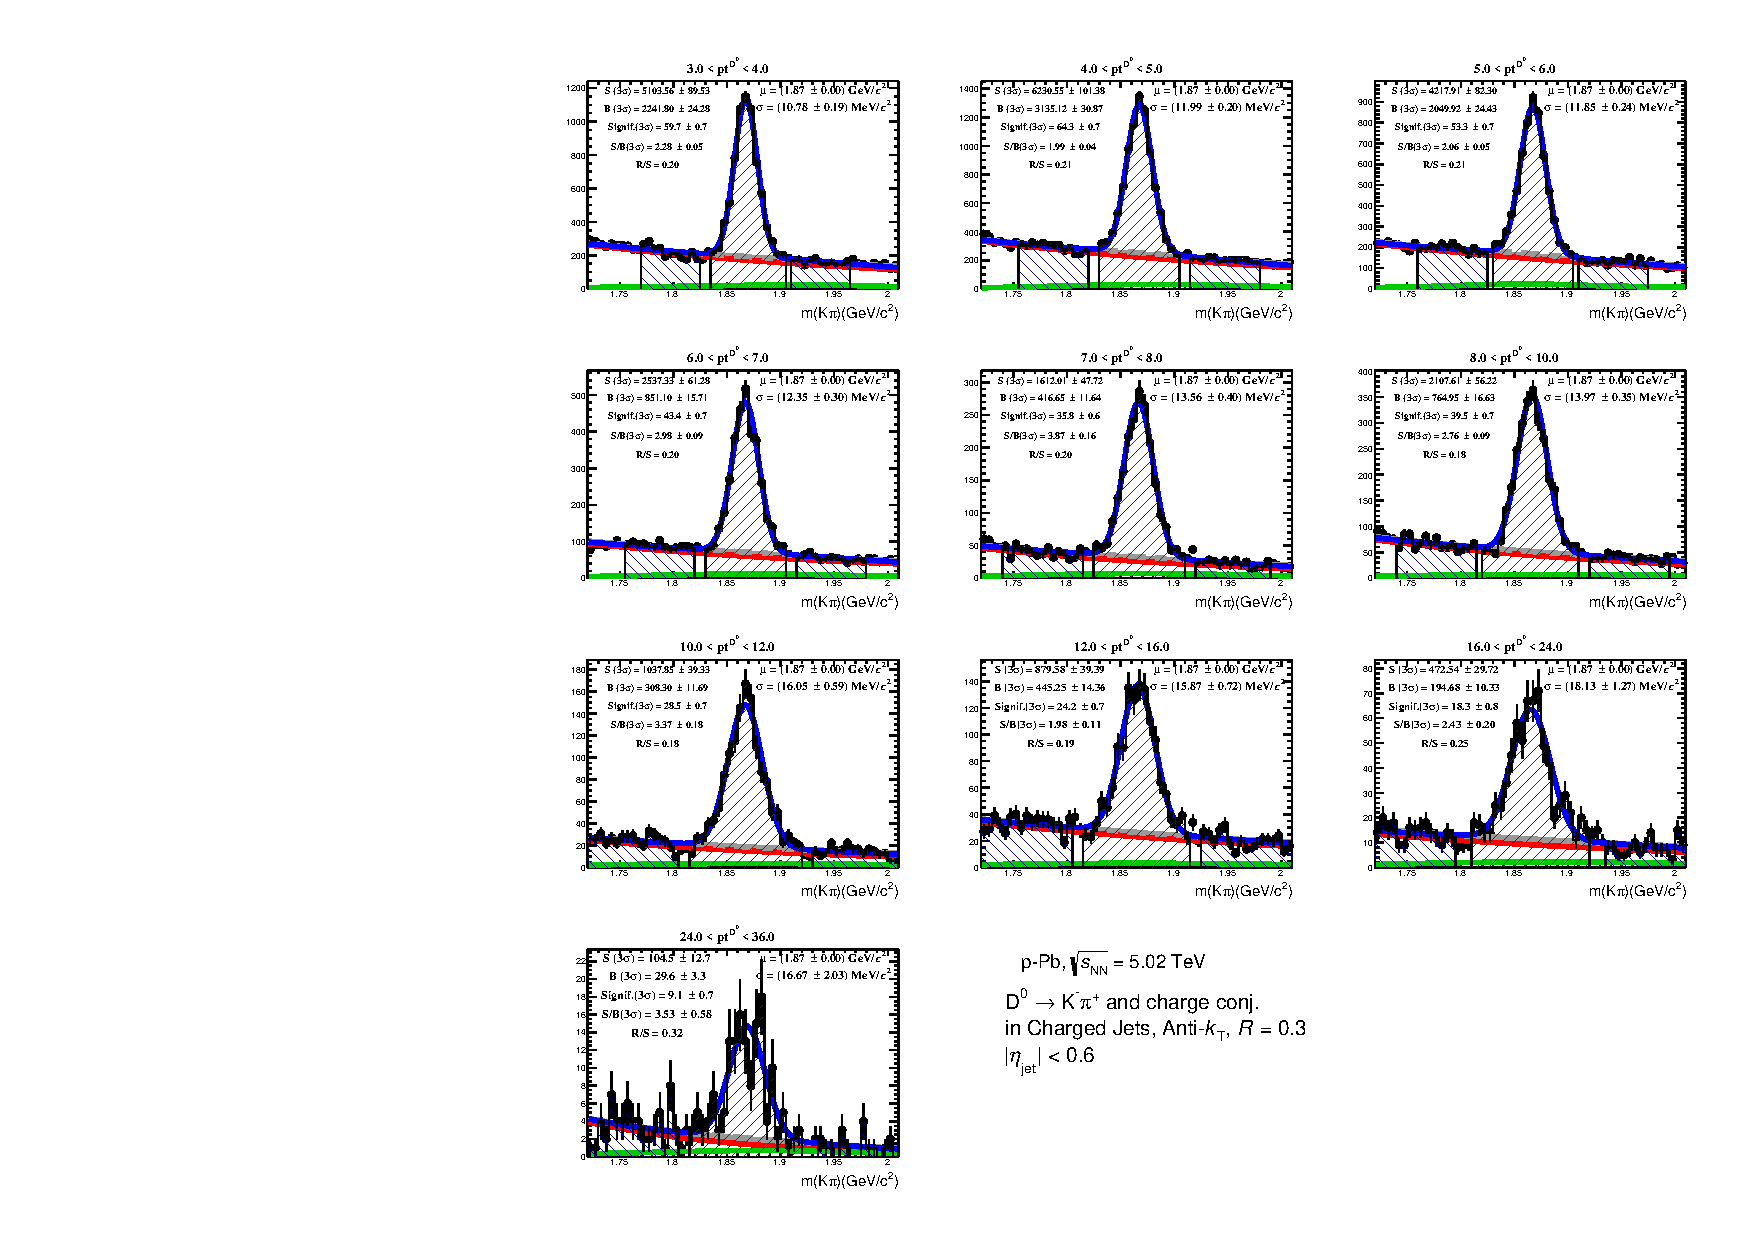
\includegraphics[width=0.9\textwidth]{pPbplotsD0/Default/signalExtraction/plots/invMass_LHC16R03_pTD3.pdf}
\caption{\Dzero-jet signal extraction in bins of jet transverse momentum in \pPb\ collisions at $\snn=5.02$~TeV (raw yields). D mesons are required to have $\pt>3$~\GeVc. 
Reflections shown by green curve add with the combinatorial background (red curve) to give the overall background in grey.
}
\label{fig:eq_pPb_InvMass_Dzero_Dbins}
\end{figure}

\begin{figure}[bth]
\centering
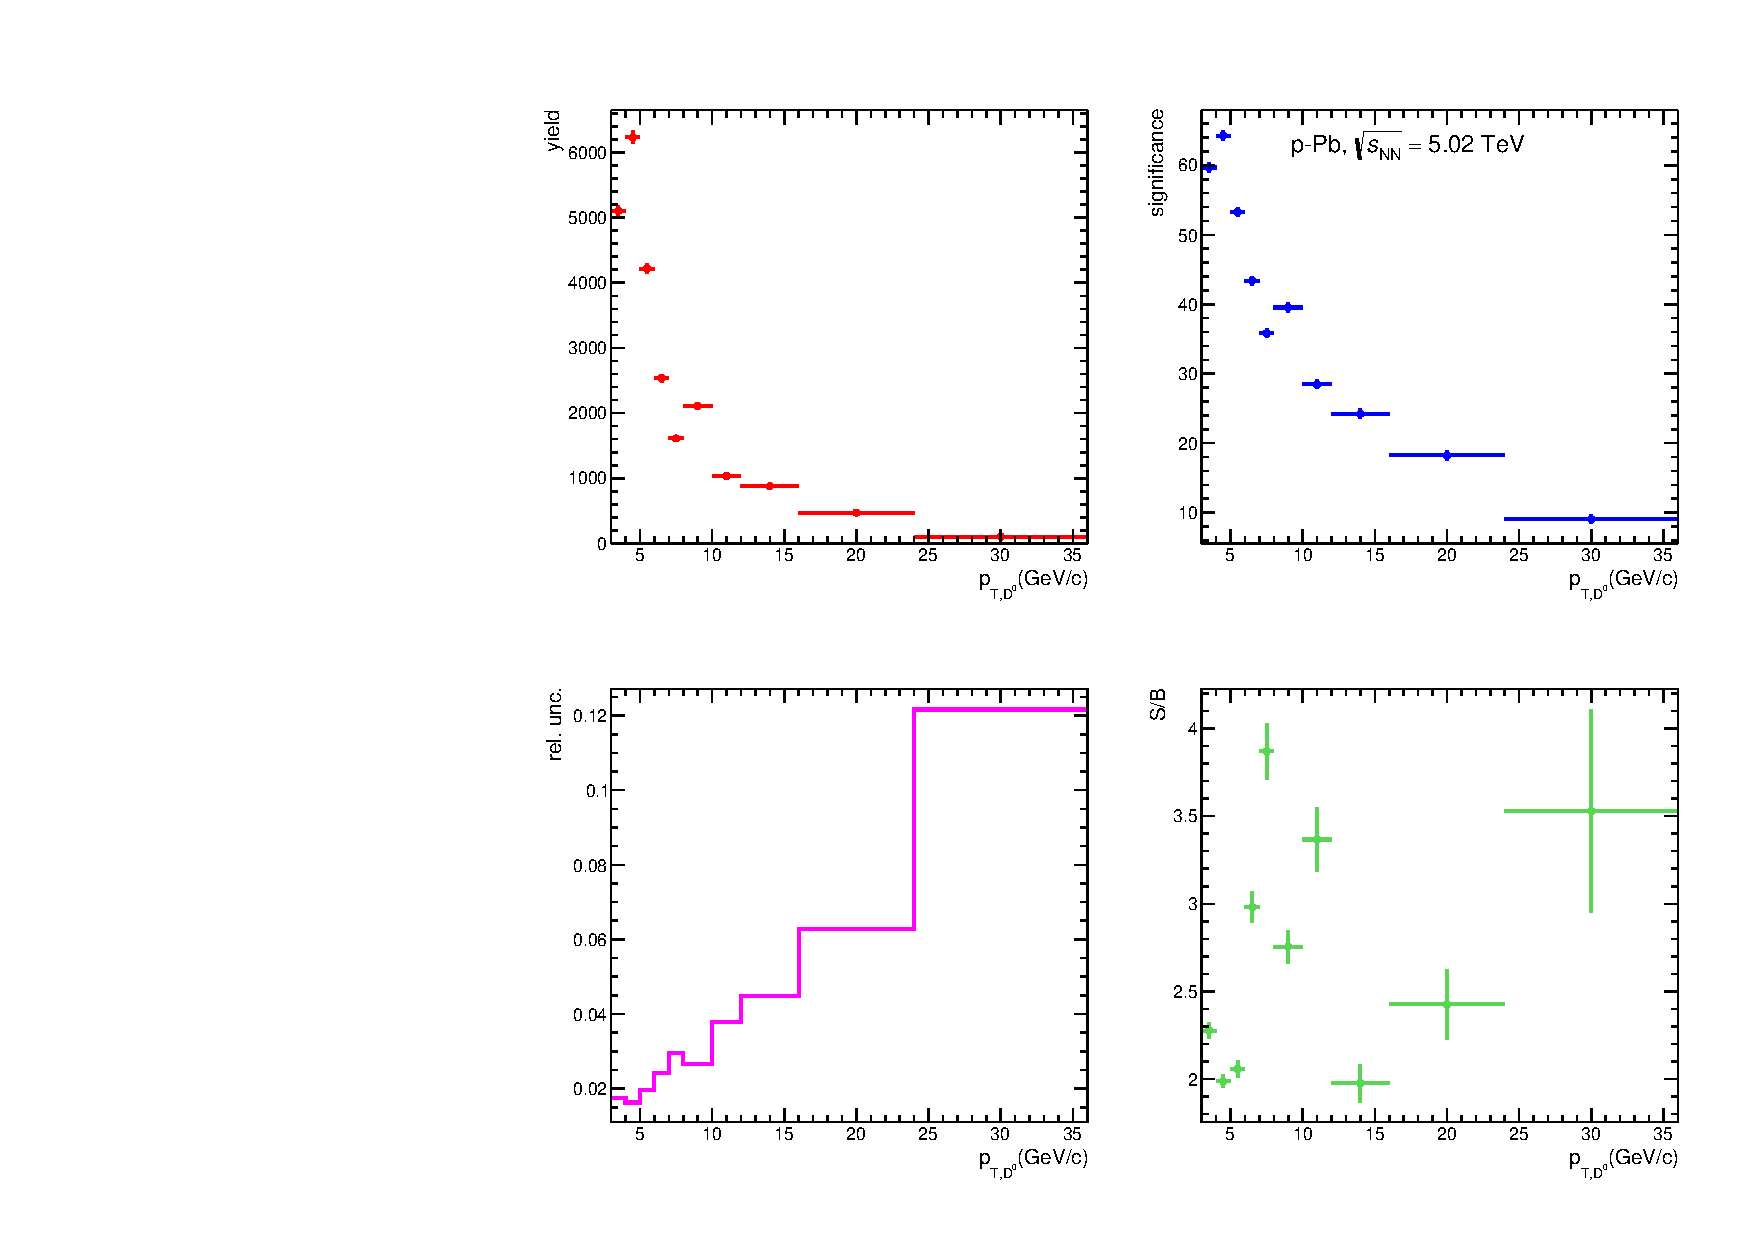
\includegraphics[width=0.64\textwidth]{pPbplotsD0/Default/signalExtraction/plots/signalParams_LHC16R03_pTD3.pdf}
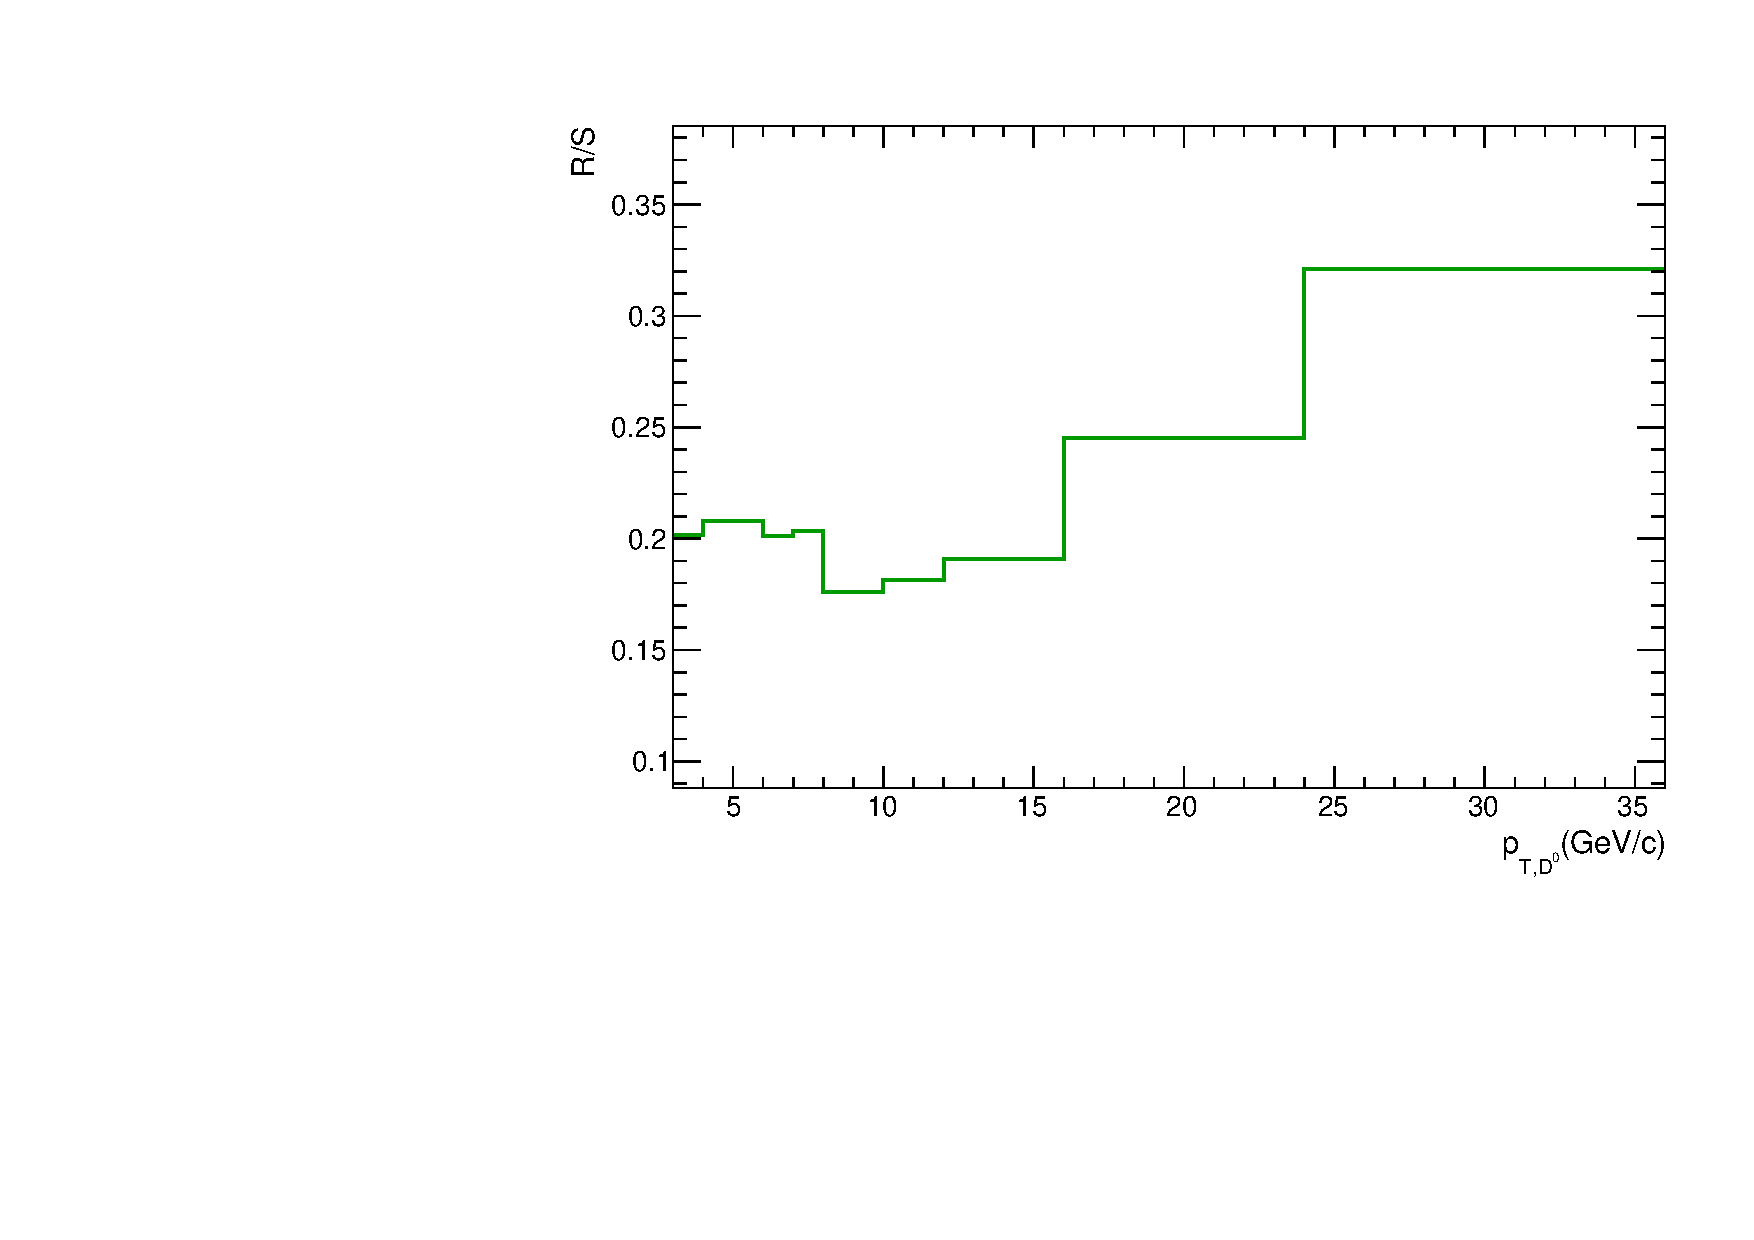
\includegraphics[width=0.35\textwidth]{pPbplotsD0/Default/signalExtraction/plots/RefOverS_LHC16R03_pTD3.pdf}
\caption{Left: \Dzero-jet raw signal extraction: raw yields, relative statistical uncertainties, significance and S/B ratio in \Dzero\ \pt\ bins, in \pPb\ collisions at $\snn=5.02$~TeV for $\ptd>3$~\GeVc\ with the Side Band method.
\\Right: \Dzero-jet raw signal extraction, reflections over signal ratio, in \pPb\ collisions at $\snn=5.02$~TeV for $\ptd>3$~\GeVc\ with the Side Band method.}
\label{fig:eq_pPb_RSU_raw_Dbins_Dzero}
\end{figure}

The raw jet \pt\ distributions for \Dstar\ are shown in Fig.~\ref{fig:eq_pPb_signBkgJet_Dstar_Dbins} and for \Dzero\ in Fig.~\ref{fig:eq_pPb_signBkgJet_Dzero_Dbins}, along with the jet \pt\ distributions for the background region. 
Then the background distributions are subtracted from the signal distributions and raw jet \pt\ distributions are obtained in each D \pt\ bin, 
as it is shown also in Fig.~\ref{fig:eq_pPb_signBkgJet_Dstar_Dbins} for \Dstar\ and in Fig.~\ref{fig:eq_pPb_signBkgJet_Dzero_Dbins} for \Dzero.
%Dstar
\begin{figure}[bth]
\centering
\includegraphics[width=0.9\textwidth]{pPbplots/plotsSB_noEff_pt3_noDetails/jetRawSpectrumFASTwoSDD_pTD3}
\caption{Raw jet \pt\ distributions in bins of \Dstar\ transverse momentum in \pPb\ collisions at $\snn=5.02$~TeV.}
\label{fig:eq_pPb_signBkgJet_Dstar_Dbins}
\end{figure}
%Dzero
\begin{figure}[bth]
\centering
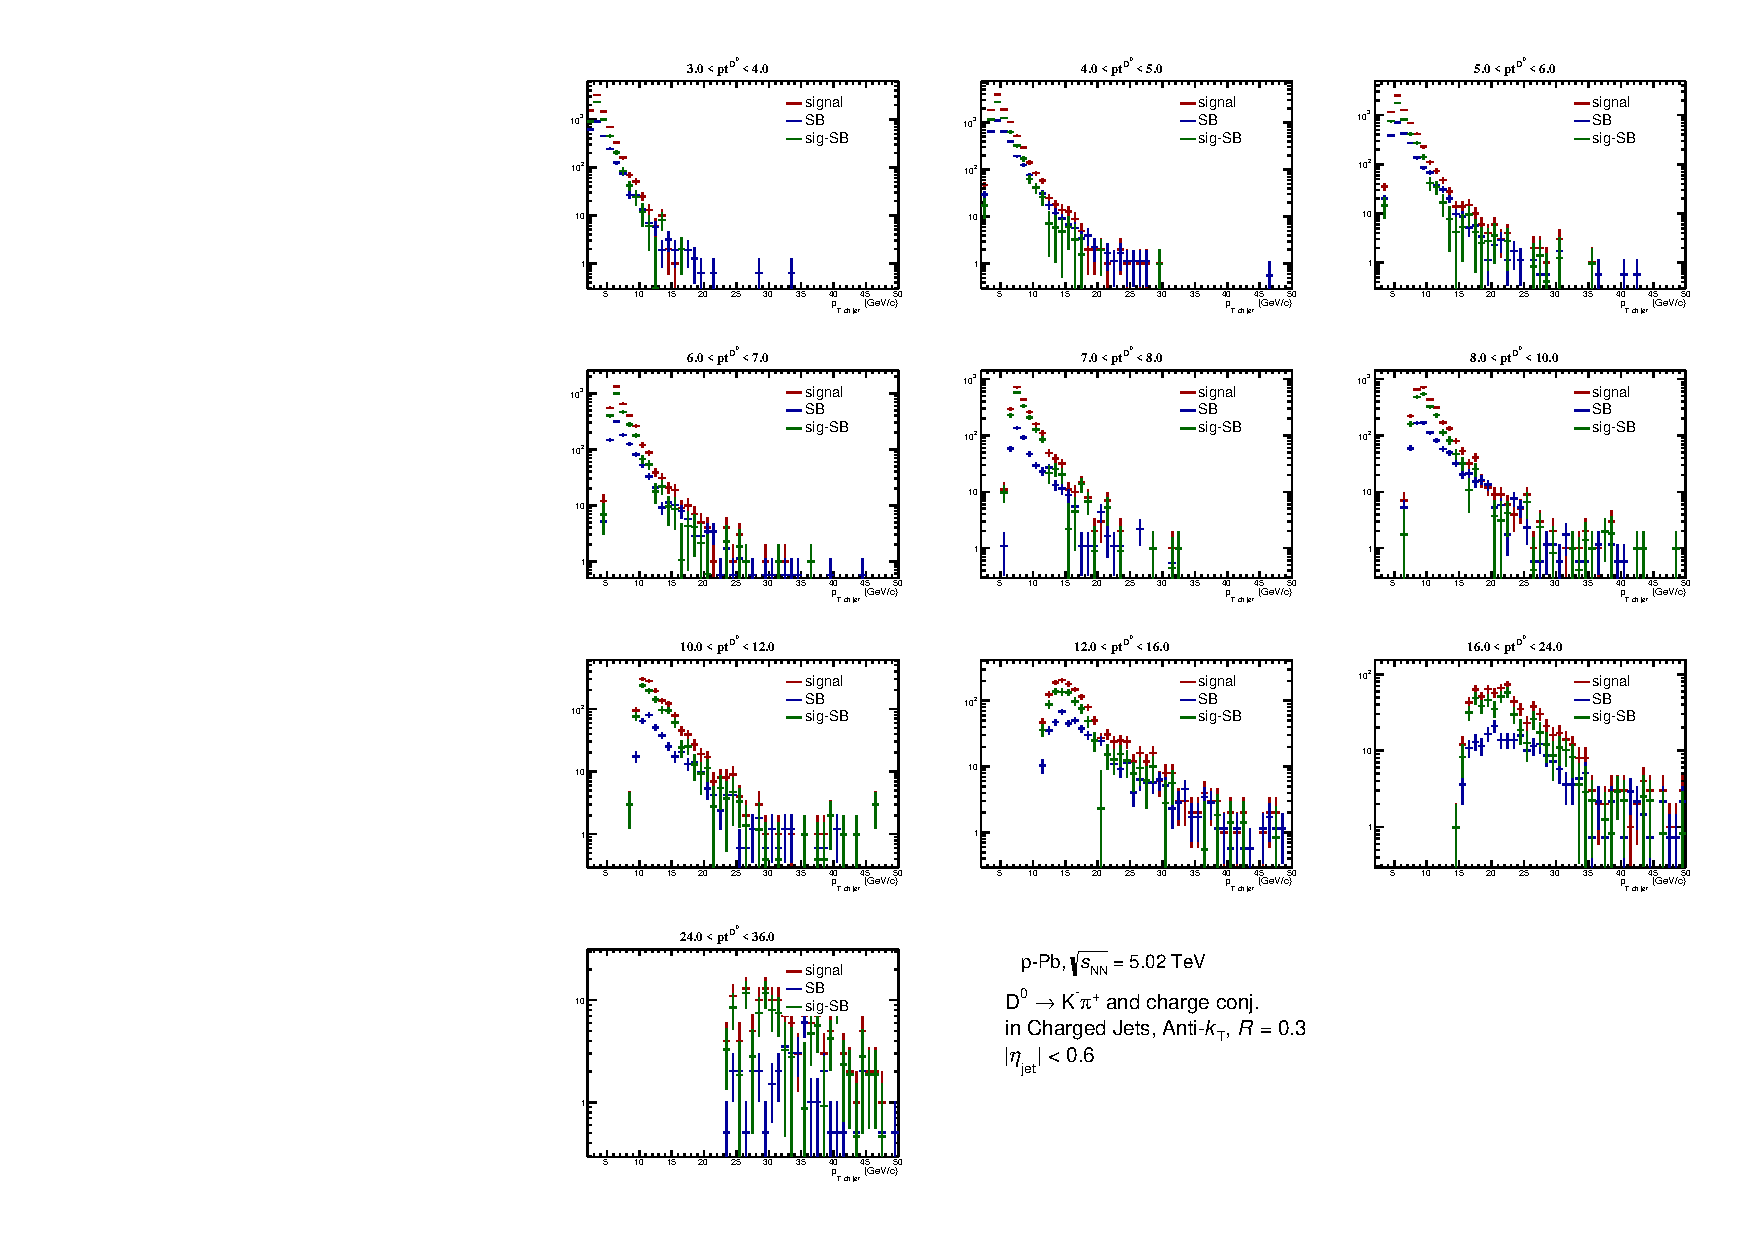
\includegraphics[width=0.9\textwidth]{pPbplotsD0/Default/signalExtraction/plots/jetRawSpectrum_LHC16R03_pTD3.pdf}
\caption{Raw jet \pt\ distributions in bins of \Dzero\ transverse momentum in \pPb\ collisions at $\snn=5.02$~TeV.}
\label{fig:eq_pPb_signBkgJet_Dzero_Dbins}
\end{figure}

Figure~\ref{fig:eq_pPb_signBkgJet_tot} and Fig.~\ref{fig:eq_pPb_signBkgJet_tot_reb} show the sum of the jet \pt\ distributions for \Dstar-jets\ (left) and \Dzero-jets\ (right) without a correction for the D-meson-jet efficiency.

%%%% signal and backgrouns scaling factors for Dzero to be added

\begin{figure}[bth]
\centering
\includegraphics[width=0.49\textwidth]{pPbplots/plotsSB_noEff_pt3_noDetails/jetPtSpectrum_SB_FASTwoSDD_pTD3}
\includegraphics[width=0.49\textwidth]{pPbplotsD0/Default/signalExtraction/plotsNoEff/jetPtSpectrum_SB_LHC16R03_pTD3.pdf}
\caption{Total raw jet \pt\ distributions for \Dstar\ (left) and \Dzero\ (right) in \pPb\ collisions at $\snn=5.02$~TeV, obtained summing together all D \pt\ bins without an efficiency correction.}
\label{fig:eq_pPb_signBkgJet_tot}
\end{figure}

\begin{figure}[bth]
\centering
\includegraphics[width=0.49\textwidth]{pPbplots/plotsSB_noEff_pt3_noDetails/jetPtSpectrum_SB_Rebin_FASTwoSDD_pTD3}
\includegraphics[width=0.49\textwidth]{pPbplotsD0/Default/signalExtraction/plotsNoEff/jetPtSpectrum_SB_Rebin_LHC16R03_pTD3.pdf}
\caption{Total raw jet \pt\ distributions for \Dstar\ (left) and \Dzero\ (right) in \pPb\ collisions at $\snn=5.02$~TeV, obtained summing together all D \pt\ bins without an efficiency correction.}
\label{fig:eq_pPb_signBkgJet_tot_reb}
\end{figure}

%
%\begin{figure}[bth]
%\centering
%\includegraphics[width=0.7\textwidth]{pPbplots/plotsSB_noEff_pt3_noDetails/signalParams_FASTwoSDD_pTD3}
%\caption{\Dstar-jet raw signal extraction in \pPb\ collisions at $\snn=5.02$~TeV for $\ptd>3$~\GeVc\ with the Side Band method.}
%\label{fig:eq_pPb_RSU_raw_Dbins_Dstar}
%\end{figure}
%
%\begin{figure}[bth]
%\centering
%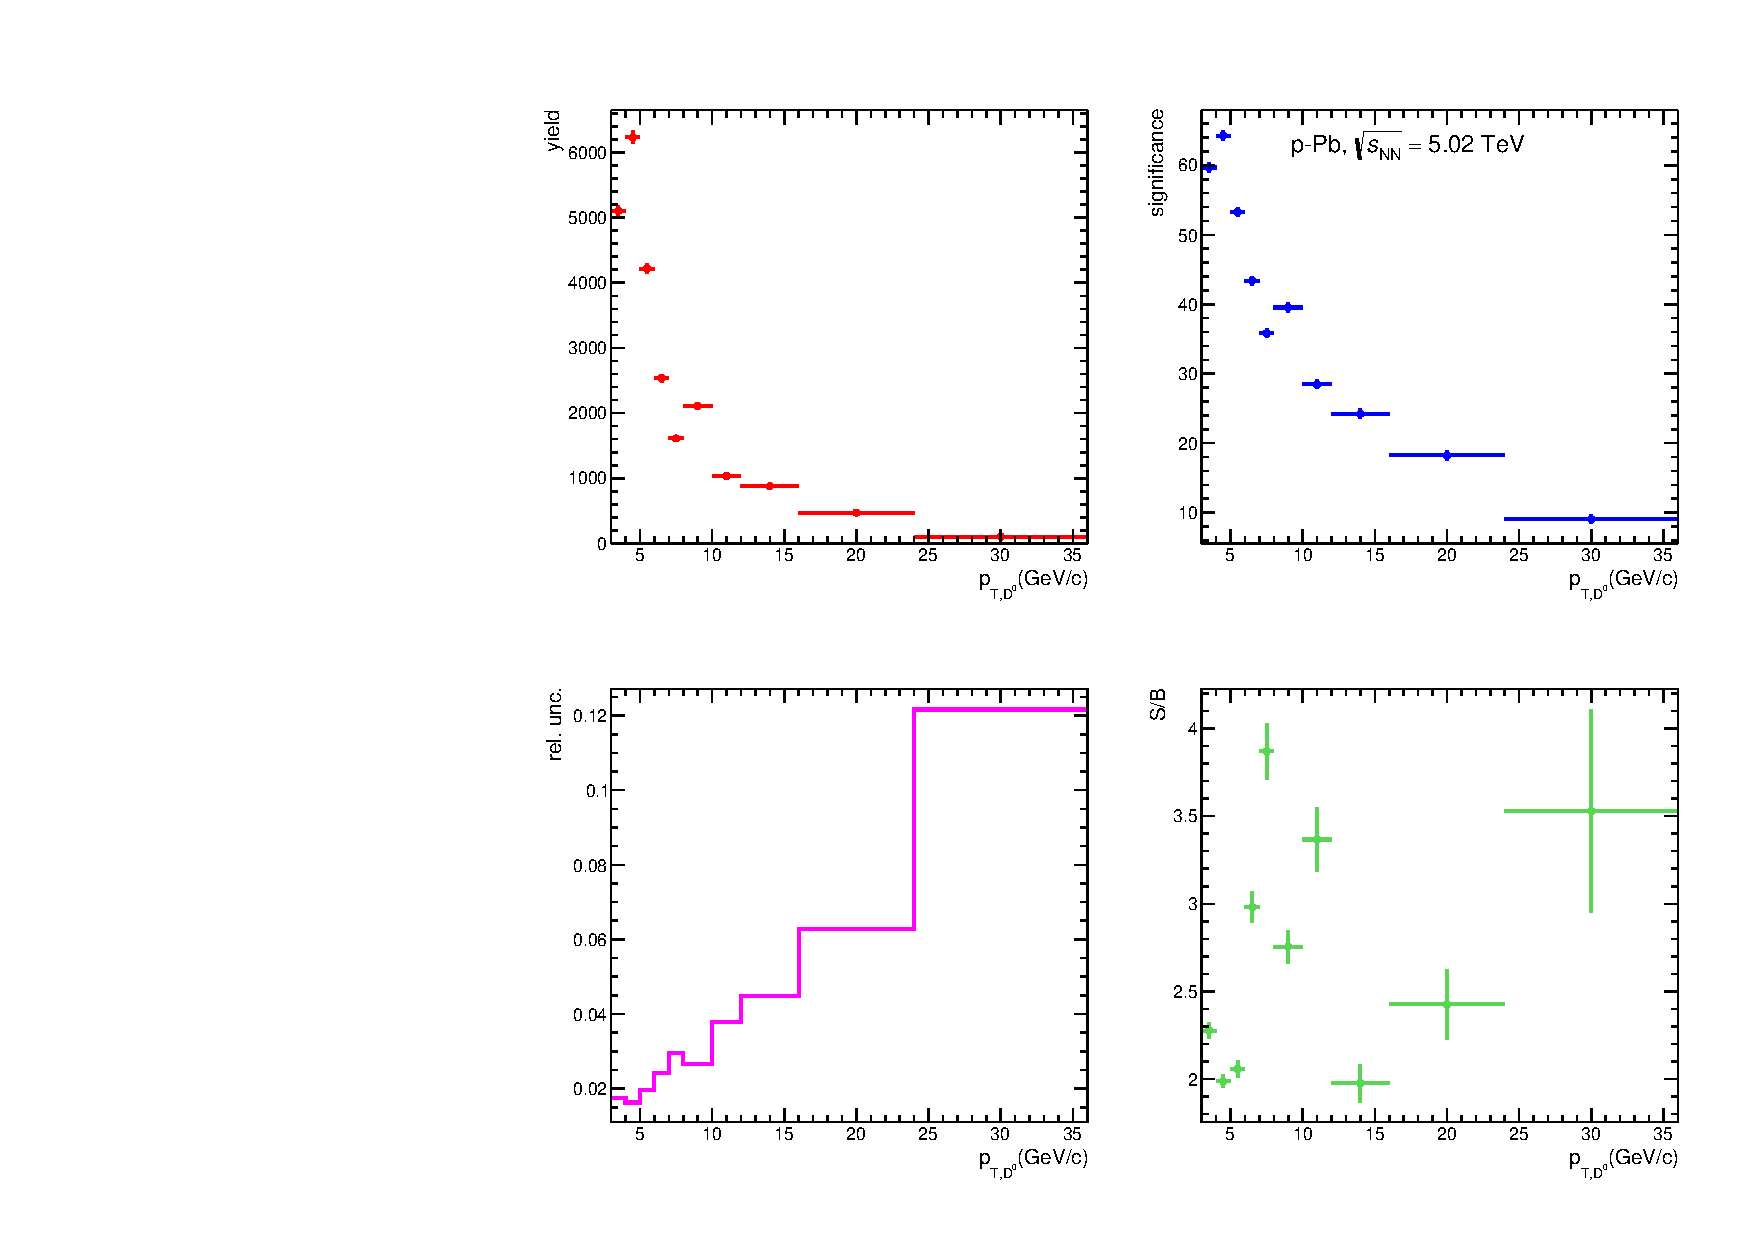
\includegraphics[width=0.7\textwidth]{pPbplotsD0/Default/signalExtraction/plots/signalParams_LHC16R03_pTD3.pdf}
%\caption{\Dzero-jet raw signal extraction in \pPb\ collisions at $\snn=5.02$~TeV for $\ptd>3$~\GeVc\ with the Side Band method.}
%\label{fig:eq_pPb_RSU_raw_Dbins_Dzero}
%\end{figure}

In order to obtain the final jet \pt\ spectrum, the distributions in each D \pt\ bin need to be corrected for the D efficiency and finally summed up.
The corrections will be discussed in Section~\ref{sect:sub_DmesonRecEff}. 
%\newpage
%\newpage
\subsection{Method Comparison}

Figure~\ref{fig:pPbCompDirectJetSB_beforeEff} shows a comparison of the raw yields (without the D-reconstruction efficiency applied). 
Jet $p_T$ spectra are checked with two cuts on the D-meson $p_{T}$: $\ptd>2$~\GeVc and $\ptd>3$~\GeVc. Both agree with each other as it is seen in Fig.~\ref{fig:pPbCompDirectJetSB_beforeEff}. 
However, it is more important to cross-check the two methods with different \ptd\ cuts after the efficiency correction is applied, 
as the background at low \ptd\ influences the analysis more, as it is shown later.

\begin{figure}[bth]
\centering
\begin{subfigure}[b]{0.45\textwidth}
\includegraphics[width=\textwidth]{pPbplots/methodsComparison/DjetSpectra_methodComparison_FASTwoSDD_noEff_ptD2}
\caption{Yields, $\ptd>2$~\GeVc}
\end{subfigure}
\begin{subfigure}[b]{0.45\textwidth}
\includegraphics[width=\textwidth]{pPbplots/methodsComparison/DjetSpectra_methodComparison_FASTwoSDD_noEff_ptD3}
\caption{Yields, $\ptd>3$~\GeVc}
\end{subfigure}
\begin{subfigure}[c]{0.45\textwidth}
\includegraphics[width=\textwidth]{pPbplots/methodsComparison/DjetSpectraRatio_FASTwoSDD_noEff_ptD2}
\caption{Ratio, $\ptd>2$~\GeVc}
\end{subfigure}
\begin{subfigure}[d]{0.45\textwidth}
\includegraphics[width=\textwidth]{pPbplots/methodsComparison/DjetSpectraRatio_FASTwoSDD_noEff_ptD3}
\caption{Ratio, $\ptd>3$~\GeVc}
\end{subfigure}
\caption{Comparison of the raw yields obtained using the invariant mass fit method and the side band method without the efficiency correction for \Dstar-jets in \pPb\ collisions at $\s=5.02$~TeV with $\ptd>2$~\GeVc (left) and $\ptd>3$~\GeVc (right).}
\label{fig:pPbCompDirectJetSB_beforeEff}
\end{figure}

%%%%%%%%%%%%%%%%%%%%%%%%%%%%%%%%%%%%%%%%%%%%%%%%%%%%%%%%%%%%%%%%%%%%%%
%%%%%%%%%%%%%%%%%%%%%%%%%%%%%%%%%%%%%%%%%%%%%%%%%%%%%%%%%%%%%%%%%%%%%%
%%%%%%%%%%%%%%%%%%%%%%%%%%%%           EFFICIENCY            %%%%%%%%%%%%%%%%%%%%%%%%%%%%
%%%%%%%%%%%%%%%%%%%%%%%%%%%%%%%%%%%%%%%%%%%%%%%%%%%%%%%%%%%%%%%%%%%%%%
%%%%%%%%%%%%%%%%%%%%%%%%%%%%%%%%%%%%%%%%%%%%%%%%%%%%%%%%%%%%%%%%%%%%%%

\section{Efficiency Correction Procedure}

\subsection{Reconstruction Efficiency}
\label{sect:sub_DmesonRecEff}
The efficiency and acceptance (${\rm Acc} \times \epsilon$) were calculated using Monte Carlo PYTHIA6+GEANT3 simulations anchored to the data.

The efficiency is taken as the ratio of the \ptd\ spectra of the D-tagged generator-level jets for which a matched
D-tagged detector-level jet was found over all the generated D-tagged jets.
For the detector-level jets, the D meson is required to be within the standard fiducial rapidity cuts.
Jets are further requested to have $|\eta_{\rm jet}| < 0.9 - R$, both at generator and detector levels.

\begin{figure}[bth]
\centering
\begin{subfigure}[c]{0.49\textwidth}
\includegraphics[width=\textwidth,height=0.8\textwidth]{pPbplots/DjetEff_Sim_log}
\caption{\Dstar-jet  reconstruction efficiency.}
\label{eq_pPb_DrecEff_Dstar}
\end{subfigure}
\begin{subfigure}[d]{0.49\textwidth}
\includegraphics[width=\textwidth,height=0.85\textwidth]{pPbplotsD0/Default_jetMeas3_50_jetTrue3_50_ppbinning/efficiency/DjetEff_Sim_log.pdf}
\caption{\Dzero-jet  reconstruction efficiency.}
\label{eq_pPb_DrecEff_Dzero}
\end{subfigure}
\caption{D-meson-jet reconstruction efficiencies in \pPb\ collisions at $\snn=5.02$~TeV, for prompt D mesons in red and non-prompt in blue.}
\label{fig:eq_pPb_DrecEff}
\end{figure}

Figures~\ref{eq_pPb_DrecEff_Dstar} and \ref{eq_pPb_DrecEff_Dzero} show the \Dstar\ and \Dzero\ reconstruction efficiencies as a function of \ptd\, 
for prompt and non-prompt D-mesons. Efficiency depends strongly on \ptd\ because of the topological cuts that are relaxed at higher momenta where the combinatorial background is smaller. 
\\In the \Dzero\ case, the shown efficiency is with a cut on \ptchjet\ of $5 < \ptchjet < 50$ \GeVc\ (range of the final \Dzero-tagged jet \pt\ spectrum) at the generator level, applied for both denominator and nominator in the efficiency calculation.

%However a very weak or no dependence on \ptchjet\ is observed for $5<\ptchjet<30$~\GeVc. From the ratios of the efficiencies in \ptchjet\ bins over the entire range, shown in Fig.~\ref{fig:eq_pp_DrecEff_ptd_ptjet} one can appreciate a hint of a small deviation, on the order of 10-20\%, for low momentum \Dzero\ (\ptd~$<5$~\GeVc) in high momentum jets. However this deviation is not statistically significant, and affects a very small fraction of the D-meson candidates.

\subsection{Efficiency-Corrected Yields}

As discussed in the previous section, the D-meson reconstruction efficiency shows a strong dependence on \ptd\ (but has very weak or no dependence on \ptjet).
Therefore, in order to reduce the dependence on the Monte Carlo simulation for what concerns jet fragmentation and momentum spectral shape,
the efficiency should be applied as a function of the D-meson momentum. In fact, each bin of \ptjet\ has contributions from D mesons with very different \ptd, which have different efficiencies.

\subsubsection{Direct Jet-$p_T$ Extraction Method}

The efficiency-rescaling procedure of the invariant mass distribution $M(\ptjet,\ptd)$ was implemented according to the following formula:
\begin{equation}
M(\ptjet) = \displaystyle\sum_{\ptd}\frac{M(\ptjet,\ptd)}{({\rm Acc} \times \epsilon)_{\ptd}}.
\end{equation}

Figure~\ref{fig:eq_pPb_Directjet_corrInv_Dstar} shows the \Dstar\ invariant mass distributions for different ranges of \ptchjet, after the efficiency reweighing procedure.
%Figures~\ref{fig:eq_pPb_Directjet_corrInv_Dstar} and \ref{fig:eq_pPb_Directjet_corrInv_Dzero} show the \Dstar\ and \Dzero\ invariant mass distributions 
for different ranges of \ptchjet, after the efficiency reweighing procedure.
%This process can increase the relative statistical uncertainty due to the large weight assigned to low-\pt\ D mesons (low reconstruction efficiency). 

%Dstar
\begin{figure}[bth]
\centering
\includegraphics[width=0.9\textwidth]{pPbplots/plotsEffScale_pt3_noDetails/invMass_FASTwoSDD}
\caption{\Dstar\ signal extraction in bins of jet transverse momentum in \pPb\ collisions at $\snn=5.02$~TeV. D mesons are required to have $\ptd>3$~\GeVc.
Each candidate is weighted by the inverse of the reconstruction efficiency, which depends on its \ptd.}
\label{fig:eq_pPb_Directjet_corrInv_Dstar}
\end{figure}

%Dzero
%\begin{figure}[bth]
%\centering
%\includegraphics[width=0.9\textwidth]{pPbplotsD0/}
%\caption{\Dzero\ signal extraction in bins of jet transverse momentum in \pPb\ collisions at $\snn=5.02$~TeV. D mesons are required to have $\ptd>3$~\GeVc.
%Each candidate is weighted by the inverse of the reconstruction efficiency, which depends on its \ptd.}
%\label{fig:eq_pPb_Directjet_corrInv_Dzero}
%\end{figure}
%

%Figure~\ref{fig:eq_pPb_RSU_raw_corrDrec} shows the yield and relative statistical uncertainties of the reconstructed D-tagged jets with the efficiency weighting with the invariant mass fit method. A comparison with ~\ref{fig:eq_pPb_RSU_raw} shows  that the relative statistical uncertainties are increased as a result of the efficiency weighting.

\subsubsection{Side-Band Subtraction Method}
In the side-band method the efficiency correction is applied by rescaling the D-jet background subtracted \pt\ spectra in Fig.~\ref{fig:eq_pPb_signBkgJet_Dstar_Dbins} and Fig.~\ref{fig:eq_pPb_signBkgJet_Dzero_Dbins}
by 1/(${\rm Acc} \times \epsilon$) in each D-meson \pt\ bin shown in Fig.~\ref{eq_pPb_DrecEff}, where $\epsilon$ is the prompt D-jet reconstruction efficiency.
The distributions are then summed up to obtain the corrected jet \pt\ spectra for D-jets. 
The efficiency corrected jet $p_{T}$ spectra are shown in Fig.~\ref{fig:eq_pPb_Directjet_corrSum_Dstar} and Fig.~\ref{fig:eq_pPb_Directjet_corrSum_Dzero} for \Dstar-jets and \Dzero-jets respectively. And after rebining in Fig.~\ref{fig:eq_pPb_Directjet_corrSum_reb}.

\begin{figure}[bth]
\centering
\begin{subfigure}[b]{0.45\textwidth}
\includegraphics[width=\textwidth]{pPbplots/plotsSB_pt3_noDetails/jetPtSpectrum_SB_FASTwoSDD_pTD3}
\label{fig:eq_pPb_Directjet_corrSum_Dstar}
\caption{\Dstar-jets}
\end{subfigure}
\begin{subfigure}[b]{0.45\textwidth}
\includegraphics[width=\textwidth]{pPbplotsD0/Default_jetMeas3_50_jetTrue3_50_ppbinning/signalExtraction/plots/jetPtSpectrum_SB_LHC16R03_pTD3.pdf}
\caption{\Dzero-jets}
\label{fig:eq_pPb_Directjet_corrSum_Dzero}
\end{subfigure}
\caption{Efficiency corrected D-jet yield obtained for the Side-Band subtraction method in \pPb\ collisions at $\snn=5.02$~TeV. D mesons are required to have 3 $< \ptd<$ 36~\GeVc.}
\label{fig:eq_pPb_Directjet_corrSum}
\end{figure}

%rebin
\begin{figure}[bth]
\centering
\begin{subfigure}[b]{0.45\textwidth}
\includegraphics[width=\textwidth]{pPbplots/plotsSB_pt3_noDetails/jetPtSpectrum_SB_Rebin_FASTwoSDD_pTD3}
\label{fig:eq_pPb_Directjet_corrSum_Dstar}
\caption{\Dstar-jets}
\end{subfigure}
\begin{subfigure}[b]{0.45\textwidth}
\includegraphics[width=\textwidth]{pPbplotsD0/Default_jetMeas3_50_jetTrue3_50_ppbinning/signalExtraction/plots/jetPtSpectrum_SB_Rebin_LHC16R03_pTD3.pdf}
\caption{\Dzero-jets}
\label{fig:eq_pPb_Directjet_corrSum_Dzero}
\end{subfigure}
\caption{Efficiency corrected D-jet yield obtained for the Side-Band subtraction method in \pPb\ collisions at $\snn=5.02$~TeV. D mesons are required to have 3 $< \ptd<$ 36~\GeVc.}
\label{fig:eq_pPb_Directjet_corrSum_reb}
\end{figure}

Figures~\ref{fig:JetPt_pPb_SBUnc_Dstar} and \ref{fig:JetPt_pPb_SBUnc_Dzero} show relative statistical uncertainties for the Side-Band subtraction method with $\ptd>3$~\GeVc for \Dstar-jets and \Dzero-jets. The \Dzero-jet measurement extents the \ptchjet\ reach to 50 \GeVc\, with the relative statistical uncertainty before the B feed-down subtraction and unfolding of 18\% in the last bin 36 $< \ptchjet <$ 50.

\begin{figure}[bth]
\centering
\begin{subfigure}[b]{0.45\textwidth}
\includegraphics[width=\textwidth]{pPbplots/plotsSB_pt3_noDetails/jetPtSpectrumUnc_SB_Rebin_FASTwoSDD_pTD3}
\caption{Statistical uncertainties for \Dstar-jets.}
\label{fig:JetPt_pPb_SBUnc_Dstar}
\end{subfigure}
\begin{subfigure}[b]{0.45\textwidth}
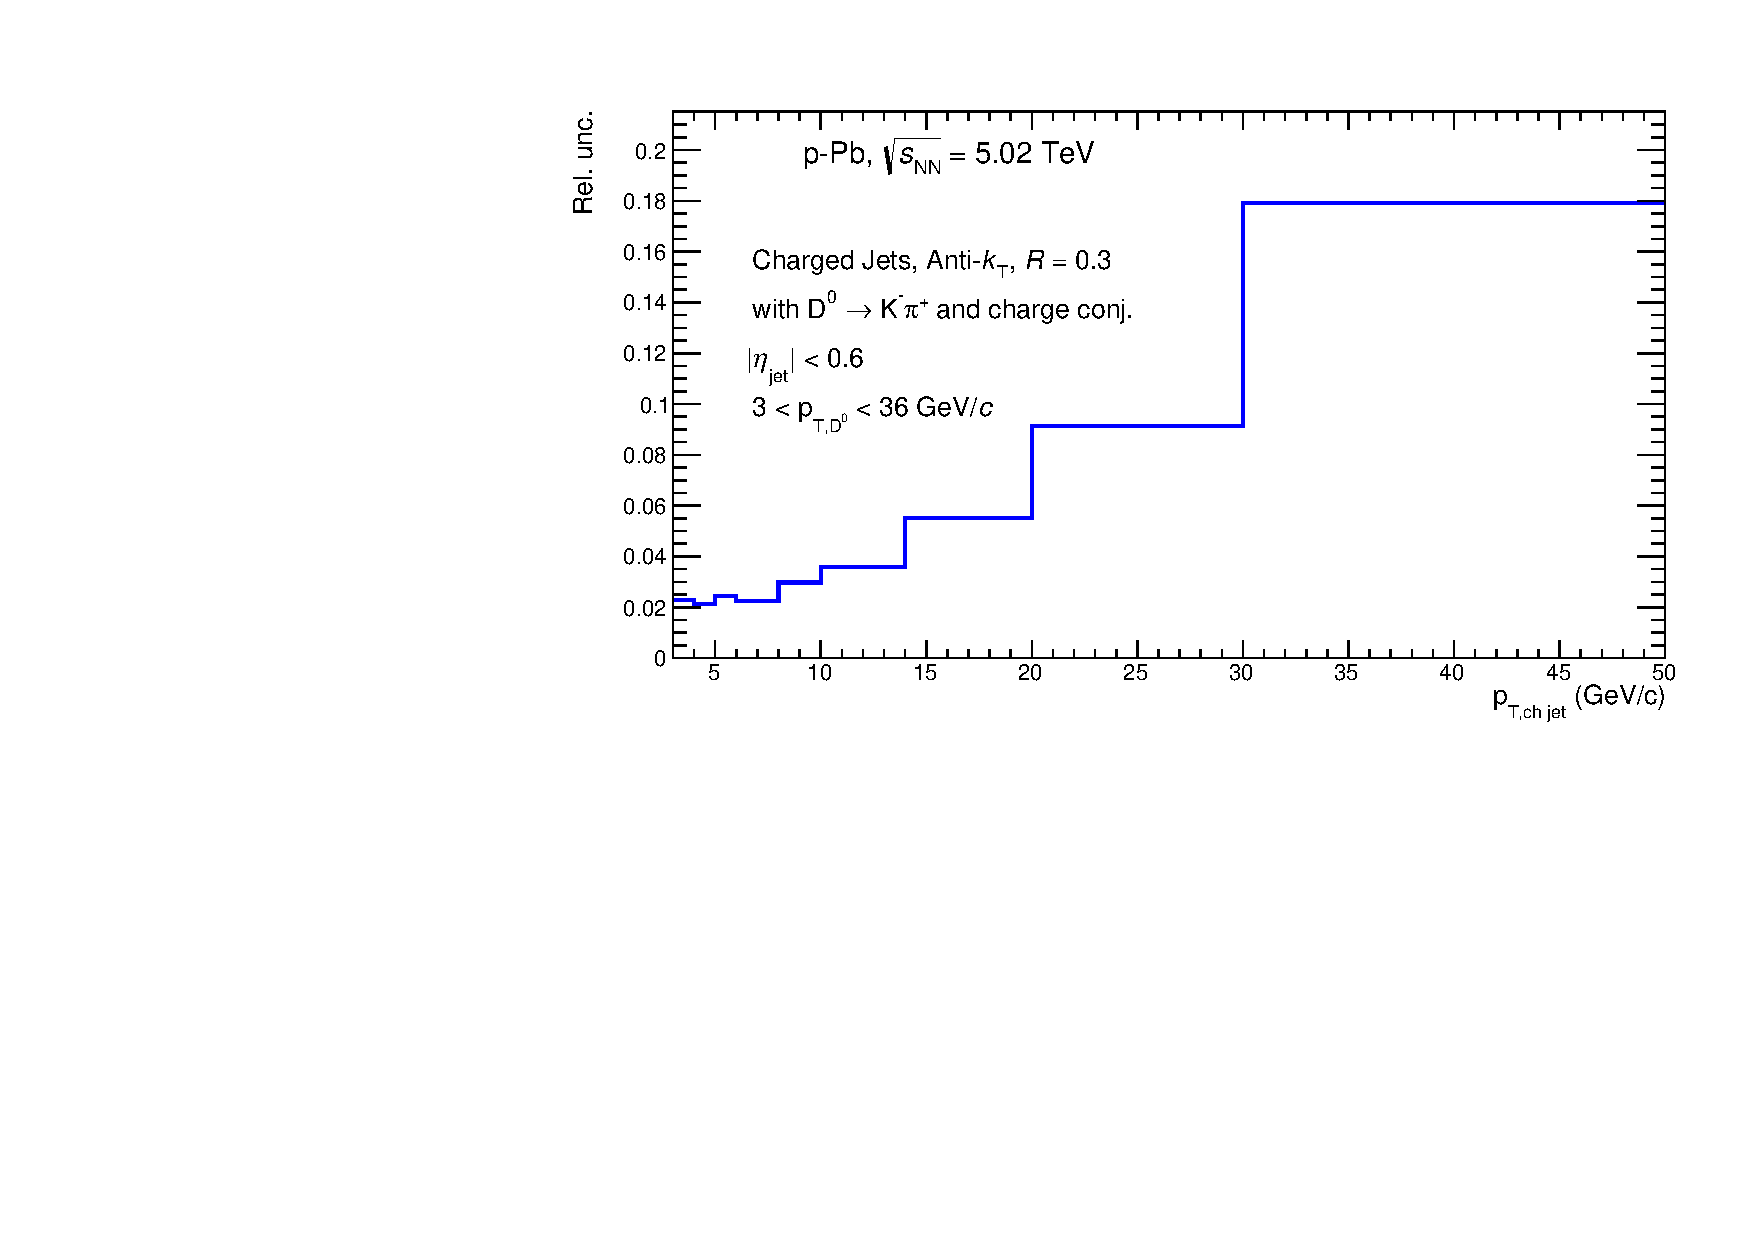
\includegraphics[width=\textwidth,height=0.8\textwidth]{pPbplotsD0/Default_jetMeas3_50_jetTrue3_50_ppbinning/signalExtraction/plots/jetPtSpectrumUnc_SB_Rebin_LHC16R03_pTD3.pdf}
\caption{Statistical uncertainties for \Dzero-jets.}
\label{fig:JetPt_pPb_SBUnc_Dzero}
\end{subfigure}
\caption{Statistical uncertainties obtained using the side band method for \Dstar-jets and \Dzero-jets in \pPb\ at $\snn=5.02$~TeV, with $\ptd>3$~\GeVc\ . Reconstruction efficiency correction is applied.}
\label{fig:JetPt_pPb_SBUnc_D}
\end{figure}


\subsection{Method Comparison (Efficiency-Corrected Yields)}

Figure~\ref{fig:JetPt_pPb_corrDrec_Dstar} shows a comparison of the efficiency-corrected yields obtained using the direct jet-\pt\ extraction method 
and the side band subtraction method for \Dstar-jets with $\ptd>2$~\GeVc\ and $\ptd>3$~\GeVc. 
%Figure~\ref{fig:JetPt_pPb_corrDrec_Dstar} and \ref{fig:JetPt_pPb_corrDrec_Dzero} show a comparison of the efficiency-corrected yields obtained using the direct jet-\pt\ extraction method and the side band subtraction method for \Dstar-jets and \Dzero-jets respectively with $\ptd>2$~\GeVc\ and $\ptd>3$~\GeVc. 
As mentioned before, the direct jet-\pt\ extraction method is sensitive to weighing with low efficiency for low $p_{T}$ D mesons. 
Therefore, discrepancies for higher \ptjet\ ranges between two methods are visible with $\ptd>2$~\GeVc\ cut. 
With $\ptd>3$~\GeVc\ cut the two methods agree very well with each other within the statistical uncertainties.
$\ptd>3$~\GeVc\ cut reduces also uncertainties on the jet spectra for higher \ptjet. 


%Figure~\ref{fig:JetPt_pPb_SBUnc} shows relative statistical uncertanties for the Side-Band subtraction method with $\ptd>2$~\GeVc\ and $\ptd>3$~\GeVc; $\ptd>3$~\GeVc\ cut reduces also uncertainties on the jet spectra for higher \ptjet. 

\begin{figure}[bth]
\centering
\begin{subfigure}[b]{0.45\textwidth}
\includegraphics[width=\textwidth]{pPbplots/methodsComparison/DjetSpectra_methodComparison_FASTwoSDD_eff_ptD2}
\caption{Yields}
\end{subfigure}
\begin{subfigure}[b]{0.45\textwidth}
\includegraphics[width=\textwidth]{pPbplots/methodsComparison/DjetSpectra_methodComparison_FASTwoSDD_eff_ptD3}
\caption{Yields}
\end{subfigure}
\begin{subfigure}[b]{0.45\textwidth}
\includegraphics[width=\textwidth]{pPbplots/methodsComparison/DjetSpectraRatio_FASTwoSDD_eff_ptD2}
\caption{Ratio}
\end{subfigure}
\begin{subfigure}[b]{0.45\textwidth}
\includegraphics[width=\textwidth]{pPbplots/methodsComparison/DjetSpectraRatio_FASTwoSDD_eff_ptD3}
\caption{Ratio}
\end{subfigure}
\caption{Comparison of the yields obtained using the direct jet-\pt\ extraction method and the side band subtraction method for \Dstar-jets in \pPb\ at $\snn=5.02$~TeV, with two cuts on \ptd: $\ptd>2$~\GeVc\ and $\ptd>3$~\GeVc.
Reconstruction efficiency correction is applied in both cases.}
\label{fig:JetPt_pPb_corrDrec_Dstar}
\end{figure}
%%Dzero
%\begin{figure}[bth]
%\centering
%\begin{subfigure}[b]{0.45\textwidth}
%\includegraphics[width=\textwidth]{pPbplotsD0/methodsComparison/}
%\caption{Yields}
%\end{subfigure}
%\begin{subfigure}[b]{0.45\textwidth}
%\includegraphics[width=\textwidth]{pPbplotsD0/methodsComparison/}
%\caption{Yields}
%\end{subfigure}
%\begin{subfigure}[b]{0.45\textwidth}
%\includegraphics[width=\textwidth]{pPbplotsD0/methodsComparison/}
%\caption{Ratio}
%\end{subfigure}
%\begin{subfigure}[b]{0.45\textwidth}
%\includegraphics[width=\textwidth]{pPbplotsD0/methodsComparison/}
%\caption{Ratio}
%\end{subfigure}
%\caption{Comparison of the yields obtained using the direct jet-\pt\ extraction method and the side band subtraction method for \Dzero-jets in \pPb\ at $\snn=5.02$~TeV, with two cuts on \ptd: $\ptd>2$~\GeVc\ and $\ptd>3$~\GeVc.
%Reconstruction efficiency correction is applied in both cases.}
%\label{fig:JetPt_pPb_corrDrec_Dzero}
%\end{figure}

{\textbf{The default method used for the further analysis is the Side Band method}} with $\ptd>3$~\GeVc\ cut. The method is more stable, Gaussian fits perform better when they are done in \ptd\ bins, since in the case of the direct Jet-$p_T$ Extraction Method the different, efficiency scaled, \ptd bins are combined together which may result in non-gaussian shape of the D-meson signal. It is easier to perform the jet spectra analysis with more fine \ptchjet\ binning if needed.

%%%%%%%%%%%%%%%%%%%%%%%%%%%%%%%%%%%%%%%%%%%%%%%%%%%%%%%%%%%%%%%%%%%%%%
%%%%%%%%%%%%%%%%%%%%%%%%%%%%%%%%%%%%%%%%%%%%%%%%%%%%%%%%%%%%%%%%%%%%%%
%%%%%%%%%%%%%%%%%%%%%%%%%%%%                   UE                     %%%%%%%%%%%%%%%%%%%%%%%%%%%%
%%%%%%%%%%%%%%%%%%%%%%%%%%%%%%%%%%%%%%%%%%%%%%%%%%%%%%%%%%%%%%%%%%%%%%
%%%%%%%%%%%%%%%%%%%%%%%%%%%%%%%%%%%%%%%%%%%%%%%%%%%%%%%%%%%%%%%%%%%%%%

\section{Underlying Event (\pPb\ analysis)}
\subsection{Average Background Momentum Density}
\label{sBackSub}

The Underlying Event (UE) affects the reconstructed jet momentum and needs to be subtracted.
The average background density $\rho$ is calculated on an event-by-event basis:

\begin{equation}
\label{eq_rho_pPB}
\rho_{\rm p-Pb} = {\rm median}\left\{\frac{p_{\rm T,jet}^{\kt}}{A_{\rm jet}^{\kt}}\right\} C.
\end{equation}
where $p_{\rm T,jet}^{\kt}$ and $A_{\rm jet}^{\kt}$ are respectively the transverse momentum and the area of
the jets found using the \kt\ algorithm. 
The jet area is estimated by \texttt{FASTJET} using the active ghost method, with a ghost area of $0.005$.
The two leading jets in the event are excluded in order to remove the hard scattering jets from the background.
This approach has been used extensively in jet reconstruction analyses~\cite{ALICE:2014a, ALICE:2015a}.
The corrected jet transverse momentum \ptchjetcorr\ is obtained by subtracting the average background density times the jet area:
\begin{equation}
\label{eq_jet_backsub}
\ptchjetcorr = \ptchjetraw - \rho A_{\rm jet}.
\end{equation}
For \pPb\ collisions a procedure that takes into account sparse environment with the factor $C$, which is the occupancy correction factor, defined as:
\begin{equation}
\label{eq_Cfac}
C = \frac{\sum_{j}A_{j}}{A_{\rm acc}}.
\end{equation}
$A_{j}$ is the area of each \kt\ jet with at least one real track (i.e. excluding ghosts), $A_{\rm acc}$ is the area of charged-particle acceptance.

Figure~\ref{fig:rho_Dstar} presents $\rho$ distributions calculated in events that include D-jet candidates (the analysed events), and requiring that an event is with the leading jet that has $p_{T}>$ 5 GeV/$c$, for 0-10\% (left) and 20-40\% (right) centrality. The distributions are compared to $\rho$ from events where a presence of D meson within a jet is not required (called inclusive-jet events).

%Dstar
\begin{figure}[bth]
\centering
\includegraphics[width=0.45\textwidth]{pPbplots/ResponseMatrix/hRho_ptleadbin5_cent0_10}
\includegraphics[width=0.45\textwidth]{pPbplots/ResponseMatrix/hRho_ptleadbin5_cent20_40}
\caption{$\rho$ distributions from events with D-jet candidates, and with a leading jet that has $p_{T}>$ 5 GeV/$c$, for 0-10\% (left) and 20-40\% (right) centrality, compared to $\rho$ from events from inclusive-jet events. \pPb\ events with $R=0.4$.}
\label{fig:rho_Dstar}
\end{figure}

\subsection{Jet Background Fluctuations}
\label{sec:BackFluc}
The amount of the jet background fluctuation was evaluated using the Random Cone method.
This method consists in generating a random direction in $\eta-\phi$ inside the jet detector acceptance and 
taking all tracks in the event that satisfy $\Delta R<R_{\rm cone}$ with $R_{\rm cone}$ equal to the resolution parameter used in the analysis. 
The raw cone \pt\ is the sum of the transverse momenta of all particles within the cone.
The background fluctuation \deltapt\ is calculated as shown in Eq.~\ref{edeltapt}, using events that include D-jet candidates excluding the leading jet in an event, and with a requirement that an event is with the leading jet $p_{T}>$ 5 GeV/$c$. The leading jet is defined as a jet with the highest \pt\ in an event.
The $\delta \pt$ distributions are shown in Fig.~\ref{fig:DeltaPt_Dstar} and Fig.~\ref{fig:DeltaPt_Dzero} on the left panels for \Dstar-jets and for \Dzero-jets, respectively. 
$\delta \pt$ distributions obtained applying different conditions are discussed in Sec.~\ref{sec:sysUnc_bkgFluctuations}.
Based on this distribution, a background fluctuation matrix is built which is then, together with the detector response matrix, used to unfold the measured D-jet \pt\ spectrum. 
The background fluctuation matrices are shown in Fig.~\ref{fig:DeltaPt_Dstar} and Fig.~\ref{fig:DeltaPt_Dzero} (right panels) for \Dstar-jets and for \Dzero-jets, respectively. 

\begin{equation}
\deltapt = p_{\rm T, cone} - \rho \pi R_{\rm cone}^{2}
\label{edeltapt}
\end{equation}

\begin{figure}[bth]
\centering
\includegraphics[width=0.45\textwidth]{pPbplots/ResponseMatrix/DeltaPt_Djet5Excl}
\includegraphics[width=0.45\textwidth]{pPbplots/ResponseMatrix/BkgMatrix_Djet5Excl}
\caption{Left: \deltapt\ distribution obtained with Random Cone method for \Dstar-jets. Right: The background fluctuation matrix built based on the \deltapt\ distribution. \pPb\ events with $R=0.4$.}
\label{fig:DeltaPt_Dstar}
\end{figure}

\begin{figure}[bth]
\centering
\includegraphics[width=0.45\textwidth]{pPbplotsD0/Default_jetMeas3_50_jetTrue3_50_ppbinning/ResponseMatrix/BkgRM03/plots/DeltaPt_Djet5Excl}
\includegraphics[width=0.45\textwidth]{pPbplotsD0/Default_jetMeas3_50_jetTrue3_50_ppbinning/ResponseMatrix/BkgRM03/plots/BkgMatrix_Djet5Excl}
\caption{Left: \deltapt\ distribution obtained with Random Cone method for \Dzero-jets. Right: The background fluctuation matrix built based on the \deltapt\ distribution. \pPb\ events with $R=0.3$.}
\label{fig:DeltaPt_Dzero}
\end{figure}


%%%%%%%%%%%%%%%%%%%%%%%%%%%%%%%%%%%%%%%%%%%%%%%%%%%%%%%%%%%%%%%%%%%%%%
%%%%%%%%%%%%%%%%%%%%%%%%%%%%%%%%%%%%%%%%%%%%%%%%%%%%%%%%%%%%%%%%%%%%%%
%%%%%%%%%%%%%%%%%%%%%%%%%%%%  DETECTOR RESPONSE  %%%%%%%%%%%%%%%%%%%%%%%%%%%%
%%%%%%%%%%%%%%%%%%%%%%%%%%%%%%%%%%%%%%%%%%%%%%%%%%%%%%%%%%%%%%%%%%%%%%
%%%%%%%%%%%%%%%%%%%%%%%%%%%%%%%%%%%%%%%%%%%%%%%%%%%%%%%%%%%%%%%%%%%%%%

\section{Jet Momentum Detector Response}

The detector response is studied with a Monte Carlo simulation in which particles generated by an event generator are
run through a transport code (GEANT3), that simulates the response of the detector elements, and then the same event reconstruction used in data is performed. Only \ccbar\ events are used.

Two sets of jets are obtained from the same event. One of them is obtained from the generator-level information and the second from the reconstructed signals after the detector simulation. 
The generated and reconstructed jets are matched by looking for the same D meson at both levels (using its MC label).


\subsection{Detector Response Matrix}
\label{Det_Resp}

The detector response matrices for prompt and non-prompt \Dstar-jets is shown in Fig.~\ref{fig:fRMdet_pPb} and for \Dzero-jets in Fig.~\ref{fig:fRMdet_pPb_Dzero}.
The Monte Carlo production is with Hijing. However, in order to avoid Hijing imperfection of describing the underlying event, 
only the Pythia part of the production is used to extract the detector response matrix, and the background fluctuations matrix is obtained from data~\ref{sBackFluc}.

\begin{figure}[bth]
\centering
\includegraphics[width=0.49\textwidth]{pPbplots/ResponseMatrix/DetMatrix_Dpt0_100}
\includegraphics[width=0.49\textwidth]{pPbplots/ResponseMatrix/DetMatrix_Dpt0_100_FD}
\caption{Detector response matrix calculated with the PYTHIA part of the simulation of \pPb\ events at $\snn=5.02$~TeV, for prompt (left) and non-prompt (right) \Dstar-jet, R=0.4.}
\label{fig:fRMdet_pPb}
\end{figure}


\begin{figure}[bth]
\centering
\includegraphics[width=0.49\textwidth]{pPbplotsD0/Default_jetMeas3_50_jetTrue3_50_ppbinning/ResponseMatrix/plots/DetMatrix_prompt_Dpt3_36}
\includegraphics[width=0.49\textwidth]{pPbplotsD0/Default_jetMeas3_50_jetTrue3_50_ppbinning/ResponseMatrix/plots/DetMatrix_nonPrompt_Dpt3_36}
\caption{Detector response matrix calculated with the PYTHIA part of the simulation of \pPb\ events at $\snn=5.02$~TeV, for prompt (left) and non-prompt (right) \Dzero-jet, R=0.3. 3 $< \ptd < $ 36~\GeVc\ .}
\label{fig:fRMdet_pPb_Dzero}
\end{figure}

For both the \Dstar-jets and \Dzero-jets, their respective prompt detector response matrices are used to unfold the measured D-jet \pt\ spectra after subtraction of the B feed-down component. 
For each D-jet, the B feed-down is estimated based on simulations, as described later, that is folded with the presented non-prompt detector response matrix combined with the background fluctuation matrix.
%
%Figure~\ref{fig:pPb_ResponseMatrixProj} shows projections of the response on the detector level jet \pt\ in bins of a particle level jet \pt.
%
%\begin{figure}[bth]
%\centering
%\includegraphics[width=0.9\textwidth]{pPbplots/ResponseMatrix/DetMatrixProjectionsComparison_Dpt3_36}
%\caption{Projections of the response on the detector level jet \pt\ in bins of a particle level jet \pt\ calculated with the Pythia simulation of \pPb\ events at $\snn=5.02$~TeV.}
%\label{fig:pPb_ResponseMatrixProj}
%\end{figure}
%
%\subsection{Jet Momentum Resolution}
%
%The jet momentum resolution and energy scale shift are estimated calculating the variable:
%\begin{equation}
%(p_{\mathrm{T,ch\, jet}}^{\mathrm{det}} - p_{\mathrm{T,ch\, jet}}^{\mathrm{part}}) / p_{\mathrm{T,ch\, jet}}^{\mathrm{part}}
%\label{eq:detResp}
%\end{equation}
%for each matched pair of a particle-level jet with a detector-level jet.
%Figure~\ref{fig:pPb_DetectorResponse} shows the probability density distribution of Eq.~\ref{eq:detResp} for \Dstar-jets in \pPb\ collisions at $\snn=5.02$~TeV.
%
%\begin{figure}[bth]
%\centering
%\includegraphics[width=0.9\textwidth]{pPbplots/ResponseMatrix/DetMatrixResProjectionsComparison}
%\caption{Jet momentum resolution calculated with a full simulation of \pPb\ events at $\snn=5.02$~TeV.}
%\label{fig:pPb_DetectorResponse}
%\end{figure}
%
%Figure~\ref{fig:pPb_ResponseMatrixProj} and~\ref{fig:pPb_DetectorResponse} include also a comparison of responses for prompt (red) and non-prompt (blue) \Dstar-jet\ production. The non-prompt response is used at the B feed-down subtraction level, as described in~\ref{sect:FD}.
%


%%%%%%%%%%%%%%%%%%%%%%%%%%%%%%%%%%%%%%%%%%%%%%%%%%%%%%%%%%%%%%%%%%%%%%
%%%%%%%%%%%%%%%%%%%%%%%%%%%%%%%%%%%%%%%%%%%%%%%%%%%%%%%%%%%%%%%%%%%%%%
%%%%%%%%%%%%%%%%%%%%%%%%%%%%           FEED-DOWN            %%%%%%%%%%%%%%%%%%%%%%%%%%%%
%%%%%%%%%%%%%%%%%%%%%%%%%%%%%%%%%%%%%%%%%%%%%%%%%%%%%%%%%%%%%%%%%%%%%%
%%%%%%%%%%%%%%%%%%%%%%%%%%%%%%%%%%%%%%%%%%%%%%%%%%%%%%%%%%%%%%%%%%%%%%

\section{Feed-Down Correction}
\label{sec:FD}

A fraction of the measured D mesons originates from the decays of B mesons. These D mesons are usually referred to as non-prompt,
to distinguish them from the prompt fraction, i.e. the ones that come directly from the fragmentation of a charm quark or decays of higher excited charm states.
The longer decay length of B mesons combined with the topological cuts applied in the D meson selection causes the reconstruction efficiency 
to be higher for the non-prompt fraction compared to the prompt fraction. This is shown in Fig.~\ref{fig:eq_pPb_DrecEff}.
As a consequence, the admixture of the prompt and non-prompt $D-jets$ is biased in a detector-specific way towards the non-prompt.
In order to make meaningful comparisons with theoretical and other experimental results one needs to either correct the bias or remove completely the non-prompt fraction and report only the prompt fraction. 
Both approaches require to use theoretical models or Monte Carlo simulations.
In ALICE the second approach has been preferred so far, and for this analysis we decided to follow it.

\subsection{Monte Carlo Simulation}

For the D-meson spectra analysis, ALICE has used FONLL~\cite{Cacciari:1998} calculations to estimate the non-prompt fraction~\cite{ALICE:2012d, ALICE:2014d, ALICE:2016a}.
In this analysis however we need to extract the B feed-down fraction also as a function of the jet kinematics, therefore this approach is not applicable.
We decided to use POWHEG~\cite{Alioli:2010}, a Monte Carlo event generator known to reasonably reproduce FONLL calculations and previous experimental results~\cite{Cacciari:2012b}.
The second part of the parton shower and the fragmentation into hadrons is provided by PYTHIA6 (Perugia-2011 tune). In addition a boost was applied in order to account for an asymmetric \pPb\ collision system. 

%We generated 25 M \ccbar\ events and 25 M \bbbar\ events for the baseline parameters: 
%$m_{\rm c} = 1.5$~\GeVcsq, $m_{\rm b} = 4.75$~\GeVcsq, $\mu_{\rm R} = \mu_{\rm F} =\mu_{0} = \sqrt{m^2+\pt^2}$,
%where $m_{\rm c}$ and $m_{\rm b}$ are receptively the charm and beauty masses, $\mu_{\rm R}$ and $\mu_{\rm F}$ are respectively the renormalization and factorization scale factors.  Used based PDF set is: CT10NLO and nPDF: EPS09NLO.
%Figures~\ref{fig:pp_POWHEGvsFONLL_ccbar} and~\ref{fig:pp_POWHEGvsFONLL_bbbar} show a comparison of the D-meson spectra generated by POWHEG+PYTHIA with a FONLL calculation, for \ccbar\ and \bbbar\ events respectively.


We generated 25 M \bbbar\ events for the baseline parameters: 
$m_{\rm b} = 4.75$~\GeVcsq, $\mu_{\rm R} = \mu_{\rm F} =\mu_{0} = \sqrt{m^2+\pt^2}$,
where $m_{\rm b}$ is the beauty masses, $\mu_{\rm R}$ and $\mu_{\rm F}$ are respectively the renormalization and factorization scale factors.  Used based PDF set is: CT10NLO and nPDF: EPS09NLO.
Variation of the simulation parameters are a source of the B feed-down subtraction systematic uncertainties.


The reconstruction of D-meson jets is performed in the POWHEG+PYTHIA6 events using the same procedure used for the main data analysis.

\subsection{Feed-Down Subtraction}
The B feed-down (FD) is subtracted from the measured D-meson jet \pt\ spectra by scaling the cross-section of D-meson jets obtained from the analysis of the POWHEG+PYTHIA simulation by the integrated luminosity of the analyzed data, according to Eq.~\ref{eq:bFDsub}:
\begin{equation}
N^{\rm c\rightarrow\Dstar}(\ptchjetdet) = 
N^{\rm c,b\rightarrow\Dstar}(\ptchjetdet) - 
R_{\rm det}^{\rm b\rightarrow\Dstar}(\ptchjetdet,\ptchjetgen) \otimes \sum_{\ptd} \frac{\epsilon^{\rm b\rightarrow\Dstar}(\ptd)}{\epsilon^{\rm c\rightarrow\Dstar}(\ptd)} N^{\rm b\rightarrow\Dstar}_{\rm POWHEG}(\ptd,\ptchjetgen),
\label{eq:bFDsub}
\end{equation}
where:
\begin{itemize}
\item $N^{\rm c\rightarrow\Dstar}(\ptchjetdet)$ is the efficiency-corrected measured yield after FD subtraction; 
\item $N^{\rm c,b\rightarrow\Dstar}(\ptchjetdet)$ is the efficiency-corrected measured yield before FD subtraction;
\item $R_{\rm det}^{\rm b\rightarrow\Dstar}(\ptchjetdet,\ptchjetgen)$ is the detector response matrix of the \pt\ of non-prompt \Dstar-jets;
\item the symbol $\otimes$ is to be interpreted as the standard product of the response matrix times the vector of the yields in bins of \ptchjetgen;
\item $\epsilon^{\rm c\rightarrow\Dstar}(\ptd)$ and $\epsilon^{\rm b\rightarrow\Dstar}(\ptd)$ are respectively the reconstruction efficiencies of prompt and non-prompt \Dstar\ mesons;
\item $N^{\rm b\rightarrow\Dstar}_{\rm POWHEG}(\ptd,\ptchjetgen)$ is the cross-section of \Dstar-jets from the POWHEG simulation scaled by the integrated luminosity of the analyzed data.
\end{itemize}
Since the measured yields are corrected for the prompt D-jet efficiency, the The POWHEG D-jet spectrum is weighted with the ratio of the non-prompt over the prompt D-jet efficiency in D-meson \pt\ bins.

The same procedure is applied in the \Dzero-jet analysis.

%Projections of prompt and non-prompt \Dstar-jets response matrices in slices \ptchjetgen are shown in Fig.~\ref{fig:pPbres_prompt_nonprompt}. There are small differences between the prompt and non-prompt response seen. 
There are differences between the prompt and non-prompt response, for this reason the FD has to be subtracted before unfolding the measured spectrum; furthermore, as illustrated in Eq.~\ref{eq:bFDsub}, the spectrum obtained from the POWHEG simulation is smeared using the response of non-prompt D-jets. 
Combined response matrix that is used to fold the simulated non-prompt spectrum is shown in Fig~\ref{fig:pPb_ResponseMatrix_nonprompt_Dstar} and Fig~\ref{fig:pPb_ResponseMatrix_nonprompt_Dzero} for \Dstar-jets and \Dzero-jets, respectively.


Figure~\ref{fig:pPbFD_corr} compares the measured \Dstar-jet \pt\ spectrum with the FD spectrum and the subtracted spectrum.
Similar procedure is also employed for \Dzero-jets. % and the combined response matrix used to fold the simulated non-prompt spectrum is shown in Fig~\ref{fig:pPb_ResponseMatrix_nonprompt_Dzero}
Figure~\ref{fig:pPbFD_corr_Dzero} compares the measured \Dzero-jet \pt\ spectrum with the FD spectrum and the subtracted spectrum.

%Dstar
\begin{figure}[bth]
\centering
\includegraphics[width=0.6\textwidth]{pPbplots/ResponseMatrix/combMatrixFD_DjetExcl5}
\caption{Combined response matrix for non-prompt \Dstar-jet in \pPb\ events at $\snn=5.02$~TeV, with R=0.4.}
\label{fig:pPb_ResponseMatrix_nonprompt_Dstar}
\end{figure}

\begin{figure}[bth]
\centering
\includegraphics[width=0.49\textwidth]{pPbplotsD0/Default_jetMeas3_50_jetTrue3_50_ppbinning/ResponseMatrix/plots/ProdMatrixFD}
\includegraphics[width=0.49\textwidth]{pPbplotsD0/Default_jetMeas3_50_jetTrue3_50_ppbinning/ResponseMatrix/plots/ProdMatrixRebinFD}
\caption{Combined response matrix for non-prompt \Dzero-jet in \pPb\ events at $\snn=5.02$~TeV, for \Dzero-jet wit R=0.3.}
\label{fig:pPb_ResponseMatrix_nonprompt_Dzero}
\end{figure}

\begin{figure}[bth]
\centering
\includegraphics[width=.53\textwidth]{pPbplots/jetSpectra/JetPtSpectra_FDsub}
\includegraphics[width=.45\textwidth]{pPbplots/jetSpectra/FDratio}
\caption{Left: Efficiency-corrected measured \Dstar-jet spectrum in \pPb\ collisions at $\snn=5.02$~TeV before FD correction (green) and after FD correction (red). The FD spectrum is also plotted (blue) with its uncertainties. Right plot shows ratio of non-prompt to inclusive \Dstar-jet spectrum.}
\label{fig:pPbFD_corr}
\end{figure}


\begin{figure}[bth]
\centering
\includegraphics[width=.53\textwidth]{pPbplotsD0/Default_jetMeas3_50_jetTrue3_50_ppbinning/FDsubtraction/plots/JetPtSpectra_FDsub.pdf}
\includegraphics[width=.45\textwidth]{pPbplotsD0/Default_jetMeas3_50_jetTrue3_50_ppbinning/FDsubtraction/plots/FDratio.pdf}
\caption{Left: Efficiency-corrected measured \Dzero-jet spectrum in \pPb\ collisions at $\snn=5.02$~TeV before FD correction (green) and after FD correction (red). The FD spectrum is also plotted (blue) with its uncertainties. Right plot shows ratio of non-prompt to inclusive \Dzero-jet spectrum.}
\label{fig:pPbFD_corr_Dzero}
\end{figure}


%%%%%%%%%%%%%%%%%%%%%%%%%%%%%%%%%%%%%%%%%%%%%%%%%%%%%%%%%%%%%%%%%%%%%%
%%%%%%%%%%%%%%%%%%%%%%%%%%%%%%%%%%%%%%%%%%%%%%%%%%%%%%%%%%%%%%%%%%%%%%
%%%%%%%%%%%%%%%%%%%%%%%%%%%%           UNFOLDING            %%%%%%%%%%%%%%%%%%%%%%%%%%%%
%%%%%%%%%%%%%%%%%%%%%%%%%%%%%%%%%%%%%%%%%%%%%%%%%%%%%%%%%%%%%%%%%%%%%%
%%%%%%%%%%%%%%%%%%%%%%%%%%%%%%%%%%%%%%%%%%%%%%%%%%%%%%%%%%%%%%%%%%%%%%

\section{Unfolding}
\label{sect:unfResults}

Due to detector finite momentum resolution and tracking inefficiency the jet \pt\ spectra measured as described
in the previous sections are distorted. In addition, in \pPb\ collisions, fluctuations in the background momentum density
introduce additional distortions. These distortions are detector-specific and do not allow a direct comparison
with theoretical models and other independent experimental results.

In order to correct for these distortions, we first need to assess the detector performance and quantify
the detector response to the D-meson jets. In addition, for the \pPb\ analysis the background fluctuations are quantified in a
fully data-driven fashion.

In \pPb\ the combined matrix used for the jet \pt\ spectra unfolding is built by multiplying the detector and background fluctuation matrices.
Then the matrix is rebinned according to the binning used for the final jet \pt\ spectra. The combined response matrix, a distribution used as a prior and the corrected jet \pt\ spectrum obtained from the data are passed to the unfolding algorithm. The algorithm returns an unfolded jet \pt spectrum. As a prior, the spectrum obtained from the Monte Carlo simulation at the generator level is used.

\subsection{\Dstar-tagged jets}
Figure~\ref{fig:pPb_ResponseMatrix} shows a combined response matrix for \Dstar-jets.
The corrected for the reconstruction efficiency and B feed-down jet \pt\ spectra before the unfolding (blue) and after the unfolding (red), for the side-band method, are presented in Fig.~\ref{fig:UnfSpec_pPb}
Unfolding is done with Bayesian and SVD (see~\ref{sUnfoldSys}) techniques using the \texttt{RooUnfold} software package. The default method is the Bayesian with five iterations. The green line represents folded back spectrum, and is compared to the measured jet spectrum before unfolding with different iterations in the Bayes unfolding - right panel of Fig.~\ref{fig:UnfSpec_pPb}, a considered in the analysis jet \pt\ range is above 5 GeV/$c$.
Comparison of unfolded spectra with different methods and priors is presented in the systematic uncertainties section. 

\begin{figure}[bth]
\centering
\includegraphics[width=0.49\textwidth]{pPbplots/ResponseMatrix/PythiaRM__Djet5Excl_2_bayes5_weight_MatrixProd}
\includegraphics[width=0.49\textwidth]{pPbplots/ResponseMatrix/PythiaRM__Djet5Excl_2_bayes5_weight_Matrix}
\caption{Combined response matrix for prompt \Dstar-jet in \pPb\ events at $\snn=5.02$~TeV, with R=0.4.}
\label{fig:pPb_ResponseMatrix}
\end{figure}

\begin{figure}[bth]
\centering
\includegraphics[width=0.55\textwidth]{pPbplots/ResponseMatrix/PythiaRM__Djet5Excl_2_bayes5_weight_UnfSpectrum}
\includegraphics[width=0.44\textwidth]{pPbplots/ResponseMatrix/PythiaRM__Djet5Excl_2_bayes5_weight_foldedRatio}
\caption{Left: Corrected jet \pt spectrum before (blue) and after (red) the unfolding procedure (Bayesian method with five iterations), \pPb\ events at $\snn=5.02$~TeV. Right: ratio to the measured spectrum to the folded for up to 10 iterations in the Bayesian unfolding, the considered jet \pt\ range is above 5 GeV/$c$.}
\label{fig:UnfSpec_pPb}
\end{figure}

\subsection{\Dzero-tagged jets}
Figure~\ref{fig:pPb_ResponseMatrix_Dzero} shows a combined response matrix for prompt \Dzero-jets.
The corrected for the reconstruction efficiency and B feed-down jet \pt\ spectra before the unfolding (blue) and after the unfolding (red), for the side-band method, are presented in Fig.~\ref{fig:UnfSpec_pPb_Dzero}.
Unfolding is done with Bayesian technique using the \texttt{RooUnfold} software package. The default method is the Bayesian with 3 iterations and \ptchjet\ ranges are 3 $< \ptchjet< $ 50 both for the generator and reconstructed level \pt\, with over/under flow bins considered in the unfolding procedure.
The green line represents refolded back spectrum, and is compared to the measured jet spectrum before unfolding with different iterations in the Bayes unfolding - right panel of Fig.~\ref{fig:unfIterations_pPb_Dzero}. Figure~\ref{fig:unfIterations_pPb_Dzero} (left) shows also unfolded spectra with next iterations compared to the default spectrum obtained with 3 iterations.
The final reported jet \pt\ range is 5 $< \ptchjet<$ 50 GeV/$c$.
Comparison of unfolded spectra with the SVD method, different \pt\ ranges for the input and unfolded spectra, and different priors are presented in the systematic uncertainties section, see~\ref{sUnfoldSys}. 

\begin{figure}[bth]
\centering
\includegraphics[width=0.49\textwidth]{pPbplotsD0/Default_jetMeas3_50_jetTrue3_50_ppbinning/ResponseMatrix/plots/ProdMatrix}
\includegraphics[width=0.49\textwidth]{pPbplotsD0/Default_jetMeas3_50_jetTrue3_50_ppbinning/ResponseMatrix/plots/ProdMatrixRebin}
\caption{Combined response matrix for prompt \Dzero-jet in \pPb\ events at $\snn=5.02$~TeV, with R=0.3.}
\label{fig:pPb_ResponseMatrix_Dzero}
\end{figure}

\begin{figure}[bth]
\centering
\includegraphics[width=0.51\textwidth]{pPbplotsD0/Default_jetMeas3_50_jetTrue3_50_ppbinning/unfolding_Bayes_3/plots/unfoldedSpectrum_UnfSpectrum.pdf}
\includegraphics[width=0.48\textwidth]{pPbplotsD0/Default_jetMeas3_50_jetTrue3_50_ppbinning/unfolding_Bayes_3/plots/unfoldedSpectrum_UnfSpectrum_unc.pdf}
\caption{Left: Corrected jet \pt spectrum before (blue) and after (red) the unfolding procedure (Bayesian method with 3 iterations), \pPb\ events at $\snn=5.02$~TeV. Right: Relative statistical uncertanties on the \Dzero-tagged jet \pt\ spectrum after unfolding.}
\label{fig:UnfSpec_pPb_Dzero}
\end{figure}

\begin{figure}[bth]
\centering
\includegraphics[width=0.49\textwidth]{pPbplotsD0/Default_jetMeas3_50_jetTrue3_50_ppbinning/unfolding_Bayes_3/plots/unfoldedSpectrum_unfRatio.pdf}
\includegraphics[width=0.49\textwidth]{pPbplotsD0/Default_jetMeas3_50_jetTrue3_50_ppbinning/unfolding_Bayes_3/plots/unfoldedSpectrum_foldedRatio.pdf}
\caption{Left: ratio of the default unfolded spectrum with 3 iteration to the unfolded spectra for up to 10 iterations in the Bayesian unfolding. Right: ratio of the measured spectrum to the refolded for up to 10 iterations in the Bayesian unfolding. The considered jet \pt\ range is above 5 GeV/$c$.}
\label{fig:unfIterations_pPb_Dzero}
\end{figure}

\begin{figure}[bth]
\centering
\includegraphics[width=0.8\textwidth]{pPbplotsD0/Default_jetMeas3_50_jetTrue3_50_ppbinning/unfolding_Bayes_3/plots/unfoldedSpectrum_Pearson.pdf}
\caption{Pearson coefficients for Bayesian unfolding.}
\label{fig:unfIterations_pPb_Dzero}
\end{figure}

\section{Systematic Uncertainties}

We considered the following sources of systematic uncertainties:

\begin{easylist}[itemize]
& Raw yield extraction
& D-Meson Selection Cuts
& B Feed-Down
& Unfolding and background fluctuation matrix
& Tracking Efficiency
& \pt\ Shape of the Monte Carlo Spectrum
\end{easylist}

\subsection{Raw Yield Extraction}
The stability and systematics of the raw yield extraction has been assessed using the \texttt{MultiTrial} framework developed by the D2H group.
This framework performs the fit of the invariant mass distribution many times varying several conditions, such us binning, fixed vs. free parameters,
background function, fit range.

\subsubsection{\Dstar-tagged jets}

The following variations were included in the assessment of the systematics for the raw yield extraction of \Dstar\ jets in \pPb:
\begin{itemize}
\item fixed $\sigma=\sigma_{\rm MC}$;
\item fixed $\sigma=1.15\sigma_{\rm MC}$
\item fixed $\sigma=0.85\sigma_{\rm MC}$
\item free $\sigma$ and fixed $m_{0}=m_{\rm PDG}$;
\item fixed $\sigma=\sigma_{\rm MC}$ and $m_{0}=m_{\rm PDG}$;
\item free $\sigma$ and free $m_{0}$;
\item background functions: power-law and power-law $\times$ exponential;
\item lower limit of fit range: $0.140$, $0.142$~\GeVcsq;
\item upper limit of fit range: $0.158$, $0.160$~\GeVcsq;
\item rebin by factor 2
\end{itemize}
Figure~\ref{fig:AverageRawYieldVsDefault_pPB} shows the average of the yields obtained in each of these variations compared with the yields obtained with default fit settings as outlined in Section~\ref{sect:raw_yield}.
The systematic uncertainties are calculated as the root-mean-square of all the yields obtained in the multi-trial fits and are shown in Fig.~\ref{fig:MultiTrialRMS_pPB}.

\begin{figure}[bth]
\begin{center}
\begin{subfigure}[b]{.45\textwidth}
\includegraphics[width=\textwidth]{pPbplots/yieldExtraction/jetPtComparison_DataMVariation_SB}
%\caption{Yields}
\label{fig:AverageRawYieldVsDefault_Yields_pPb}
\end{subfigure}
\begin{subfigure}[b]{.45\textwidth}
\includegraphics[width=\textwidth]{pPbplots/yieldExtraction/SBRatio}
%\caption{Yield from multi-trial}
\label{fig:MultiTrialSys_pPb}
\end{subfigure}
\caption{\Dstar-jet yields in \pPb\ collisions obtained  with the side-band method.
On the left, the yields are shown with the default fit conditions (full markers) with error bars representing the statistical uncertainty and with the average of
the multi-trial fit with filled rectangles representing the RMS of all the multi-trial yields; on the right a ratio of the central values obtained from the raw yield extraction procedure compared the yields obtained with default fit settings as outlined in Section~\ref{sect:raw_yield}. } 
\label{fig:AverageRawYieldVsDefault_pPB}
\end{center}
\end{figure}

\begin{figure}[bth]
\begin{center}
\includegraphics[width=0.5\textwidth]{pPbplots/yieldExtraction/YieldExtSysUnc_SB}
\caption{\Dstar-jet. The RMS of the multi-trial (systematic uncertainties).} 
\label{fig:MultiTrialRMS_pPB}
\end{center}
\end{figure}

Figure~\ref{fig:MultiTrialSB_trials_pPB} shows average of the multi-trial procedure for the side-band method as a function of jet \pt\ for each \Dstar\ \pt\ bin scaled by the corresponding efficiency, and average of the all \Dstar\ \pt\ bins (blue). 
%And the Fig.~\ref{fig:MultiTrialSB_alltrials_pPB} presents variations of all considered trials, as a function of jet \pt .
%Variations of all trials as a function of jet \pt\ for each \Dstar\ \pt\ bin and scaled by the corresponding efficiency are shown in Fig~\ref{fig:MultiTrialSB_allDptVairations_pPB}.

\begin{figure}[bth]
\begin{center}
\begin{subfigure}[b]{.45\textwidth}
\includegraphics[width=\textwidth]{pPbplots/yieldExtraction/yieldInDbins}
\end{subfigure}
\begin{subfigure}[b]{.45\textwidth}
\includegraphics[width=\textwidth]{pPbplots/yieldExtraction/yieldInDbins_log}
\end{subfigure}
\caption{Average of the multi-trial procedure for the side-band method as a function of jet \pt\ for each \Dstar\ \pt\ bin scaled by the corresponding efficiency, and average of the all \Dstar \pt bins (blue).} 
\label{fig:MultiTrialSB_trials_pPB}
\end{center}
\end{figure}

\subsubsection{\Dzero-tagged jets}

The following variations were included in the assessment of the systematics for the raw yield extraction of \Dzero jets in \pPb:
\begin{itemize}
\item fixed $\sigma=\sigma_{\rm MC}$;
\item fixed $\sigma=1.15\sigma_{\rm MC}$
\item fixed $\sigma=0.85\sigma_{\rm MC}$
\item free $\sigma$ and fixed $m_{0}=m_{\rm PDG}$;
\item fixed $\sigma=\sigma_{\rm MC}$ and $m_{0}=m_{\rm PDG}$;
\item free $\sigma$ and free $m_{0}$;
\item background functions: exponential, linear, second-order polynomial;
\item lower limit of fit range: $1.72$, $1.74$~\GeVcsq;
\item upper limit of fit range: $2.00$, $2.03$~\GeVcsq;
\item rebin by factor 2
\end{itemize}


Figure~\ref{fig:MultiTrialSB_trials_pPB_Dzero} shows average of the multi-trial procedure for the side-band method as a function of jet \pt\ for each \Dzero \pt\ bin scaled by the corresponding efficiency, and average of the all \Dzero\ \pt\ bins (blue). 
Variations of all trials as a function of jet \pt\ for each \Dzero\ \pt\ bin and scaled by the corresponding efficiency are shown in Fig~\ref{fig:MultiTrialSB_allDptVairations_pPB_Dzero}.

\begin{figure}[bth]
\begin{center}
\begin{subfigure}[b]{.48\textwidth}
\includegraphics[width=\textwidth]{pPbplotsD0/Default_jetMeas3_50_jetTrue3_50_ppbinning/systematics/YieldExtraction/plots/JetPtTrialsAVDBins}
\end{subfigure}
\begin{subfigure}[b]{.48\textwidth}
\includegraphics[width=\textwidth]{pPbplotsD0/Default_jetMeas3_50_jetTrue3_50_ppbinning/systematics/YieldExtraction/plots/JetPtTrialsAvDBins_log}
\end{subfigure}
\caption{Average of the multi-trial procedure for the side-band method as a function of jet \pt\ for each \Dzero\ \pt\ bin scaled by the corresponding efficiency, and average of the all \Dzero\ \pt\ bins (blue).} 
\label{fig:MultiTrialSB_trials_pPB_Dzero}
\end{center}
\end{figure}

\begin{figure}[bth]
\begin{center}
\includegraphics[width=0.32\textwidth]{pPbplotsD0/Default_jetMeas3_50_jetTrue3_50_ppbinning/systematics/YieldExtraction/plots/JetPtTrialsDPt0_log.pdf}
\includegraphics[width=0.32\textwidth]{pPbplotsD0/Default_jetMeas3_50_jetTrue3_50_ppbinning/systematics/YieldExtraction/plots/JetPtTrialsDPt1_log.pdf}
\includegraphics[width=0.32\textwidth]{pPbplotsD0/Default_jetMeas3_50_jetTrue3_50_ppbinning/systematics/YieldExtraction/plots/JetPtTrialsDPt2_log.pdf}
\includegraphics[width=0.32\textwidth]{pPbplotsD0/Default_jetMeas3_50_jetTrue3_50_ppbinning/systematics/YieldExtraction/plots/JetPtTrialsDPt3_log.pdf}
\includegraphics[width=0.32\textwidth]{pPbplotsD0/Default_jetMeas3_50_jetTrue3_50_ppbinning/systematics/YieldExtraction/plots/JetPtTrialsDPt4_log.pdf}
\includegraphics[width=0.32\textwidth]{pPbplotsD0/Default_jetMeas3_50_jetTrue3_50_ppbinning/systematics/YieldExtraction/plots/JetPtTrialsDPt5_log.pdf}
\includegraphics[width=0.32\textwidth]{pPbplotsD0/Default_jetMeas3_50_jetTrue3_50_ppbinning/systematics/YieldExtraction/plots/JetPtTrialsDPt6_log.pdf}
\includegraphics[width=0.32\textwidth]{pPbplotsD0/Default_jetMeas3_50_jetTrue3_50_ppbinning/systematics/YieldExtraction/plots/JetPtTrialsDPt7_log.pdf}
\includegraphics[width=0.32\textwidth]{pPbplotsD0/Default_jetMeas3_50_jetTrue3_50_ppbinning/systematics/YieldExtraction/plots/JetPtTrialsDPt8_log.pdf}
\caption{Variations of all trials as a function of jet \pt\ for each \Dzero\ \pt\ bin and scaled by the corresponding efficiency.} 
\label{fig:MultiTrialSB_allDptVairations_pPB_Dzero}
\end{center}
\end{figure}

The systematic uncertainties are calculated as the root-mean-square of all the yields obtained in the multi-trial fits and are shown in Fig.~\ref{fig:MultiTrialRMS_pPB_Dzero}.
\begin{figure}[bth]
\begin{center}
\includegraphics[width=0.5\textwidth]{pPbplotsD0/Default_jetMeas3_50_jetTrue3_50_ppbinning/systematics/YieldExtSysUnc_SB.pdf}
\caption{\Dzero-jet systematic uncertanties, RMS.} 
\label{fig:MultiTrialRMS_pPB_Dzero}
\end{center}
\end{figure}


\textbf{Variation of signal and side-band ranges}

As an additional systematic unceratnty, variations of ranges of the signal and side-band definitions in the invariant-mass fit procedure are considered.
Figure~\ref{fig:JetPtSys_Dzero_SBvariaton} shows ratios of efficiency and B feed-down corrected yields to the central value and RMS of the variations.

\begin{figure}[bth]
\begin{center}
\includegraphics[width=0.49\textwidth]{pPbplotsD0/Default_jetMeas3_50_jetTrue3_50_ppbinning/systematics/SBRangesComparison_ratio.pdf}
\includegraphics[width=0.49\textwidth]{pPbplotsD0/Default_jetMeas3_50_jetTrue3_50_ppbinning/systematics/SBRangesComparison_rms.pdf}
\caption{\Dzero-jet. Left:Systematic unceratnties from the variation of definitions of the signal and side-band regions. Right: Systematic uncertanty: RMS.} 
\label{fig:JetPtSys_Dzero_SBvariaton}
\end{center}
\end{figure}


\textbf{Variation of reflection to signal ratio}

By default, the ratio reflection/signal is a fixed parameter in the fit and is taken from the MC simulation. The reflection/signal ratio is varied to estimate the
systematic uncertainty. Consider variations are $\pm$ 50\% of the default value. Systematic uncertanties arising from these variation on the final unfolded jet \pt\ spectra are 1-3\%, as shown in Fig.~\ref{fig:JetPtSys_Dzero_Refl}.

\begin{figure}[bth]
\begin{center}
\includegraphics[width=0.49\textwidth]{pPbplotsD0/Default_jetMeas3_50_jetTrue3_50_ppbinning/systematics/RawYield_reflections_ratio.pdf}
\includegraphics[width=0.49\textwidth]{pPbplotsD0/Default_jetMeas3_50_jetTrue3_50_ppbinning/systematics/RawYield_reflections_sys.pdf}
\caption{\Dzero-jet. Left:Ratio of unfolded jet \pt\ spectrum with $\pm$ 50\% variatitions of the reflection/signal ratio. Right: Systematic uncertanity, maximum of the variations in each bin.} 
\label{fig:JetPtSys_Dzero_Refl}
\end{center}
\end{figure}


The uncertanties are added in quadratures in order to obtain the final systematic uncertainty on the raw yield extraction. 

\subsection{D-Meson Selection Cuts}
Uncertainties of the D-meson cut selection is estimated by varying applied in the analysis D-meson selection criteria, as reported in~\ref{sec:DmesonSel}. 

\subsubsection{\Dstar-tagged jets}

Four variations are considered, two looser sets and two tighter sets of cuts with $\pm$10\% and $\pm$15\% variation from a default cut value. Raw \Dstar-jet \pt\ distributions with these different cut sets and corresponding \Dstar-jet efficiencies are shown in Fig.~\ref{fig:JetPtRawSys}, and ratios in Fig.~\ref{fig:JetPtRawSysRatio}.

\begin{figure}[bth]
\begin{center}
\includegraphics[width=0.49\textwidth]{pPbplots/jetSpectra/jetRawSpectra_pTD_pTD3}
\includegraphics[width=0.49\textwidth]{pPbplots/jetSpectra/efficiencies}
\caption{\Dstar-jet. Left: \Dstar-jet \pt\ distributions with different cut sets for systematic uncertainties estimation. Right: corresponding \Dstar-jet efficiencies.} 
\label{fig:JetPtRawSys}
\end{center}
\end{figure}

\begin{figure}[bth]
\begin{center}
\includegraphics[width=0.49\textwidth]{pPbplots/jetSpectra/jetRawSpectraRatio_pTD_pTD3}
\includegraphics[width=0.49\textwidth]{pPbplots/jetSpectra/efficienciesRatio}
\caption{\Dstar-jet. Left: Ratios of \Dstar-jet \pt\ distributions with different cut sets for systematic uncertainties estimation. Right: ratios of the corresponding \Dstar-jet efficiencies.} 
\label{fig:JetPtRawSysRatio}
\end{center}
\end{figure}

Corrected for the corresponding efficiency \Dstar-jet \pt\ distributions are presented in Fig.~\ref{fig:JetPtSys}. Systematic uncertainties are estimated by taking ratio of the efficiency-corrected \Dstar-jet \pt\ distributions with different cut variations to the \Dstar-jet \pt\ spectrum obtained with the default cut set and taking RMS of them, as shown in Fig

\begin{figure}[bth]
\begin{center}
\includegraphics[width=0.49\textwidth]{pPbplots/jetSpectra/jetSpectra_pTD_pTD3}
\caption{\Dstar-jet. Efficiency-corrected \Dstar-jet \pt\ distributions with different cut sets for systematic uncertainties estimation.} 
\label{fig:JetPtSys}
\end{center}
\end{figure}

\begin{figure}[bth]
\begin{center}
\includegraphics[width=0.49\textwidth]{pPbplots/jetSpectra/jetSpectraRatio_pTD_pTD3}
\includegraphics[width=0.49\textwidth]{pPbplots/jetSpectra/jetSpectraSys_pTD_pTD3}
\caption{\Dstar-jet. Left: Ratio of the efficiency-corrected \Dstar-jet \pt\ distributions with different cut sets for systematic uncertainties estimation. Right: RMS - systematic uncertainties.} 
\label{fig:JetPtSys}
\end{center}
\end{figure}

\subsubsection{\Dzero-tagged jets}

7 variations of cut selection are considered, 4 looser sets and 3 tighter sets of cuts. The variations are choosen so that they vary \Dzero reconstruction efficiency to high enough extend so that a possible imperfection in MC simulation can be probe. Though at high \ptd\ the selection criteria are already rather loose.
Raw \Dzero-jet \pt\ distributions with these different cut sets and corresponding \Dzero-jet efficiencies are shown in Fig.~\ref{fig:JetPtRawSys_Dzero}, and ratios to the default set of cuts in Fig.~\ref{fig:JetPtRawSysRatio_Dzero}.
Figure~\ref{fig:JetcutVarFD_Dzero} shows non-prompt \Dzero-jet reconstruction efficiencies for all the cut variations, and the variations of the FD fraction in the inclusive \Dzero-jet spectrum.

\begin{figure}[bth]
\begin{center}
\includegraphics[width=0.49\textwidth]{pPbplotsD0/Default_jetMeas3_50_jetTrue3_50_ppbinning/systematics/CutVariationSyst_reg0_RawSpectra.pdf}
\includegraphics[width=0.49\textwidth]{pPbplotsD0/Default_jetMeas3_50_jetTrue3_50_ppbinning/systematics/CutVariationSyst_reg0_PromptEfficiencies.pdf}
\caption{\Dzero-jet. Left: \Dzero-jet \pt\ distributions with different cut sets for systematic uncertainties estimation. Right: corresponding prompt \Dzero-jet efficiencies.} 
\label{fig:JetPtRawSys_Dzero}
\end{center}
\end{figure}

\begin{figure}[bth]
\begin{center}
\includegraphics[width=0.49\textwidth]{pPbplotsD0/Default_jetMeas3_50_jetTrue3_50_ppbinning/systematics/CutVariationSyst_reg0_RawSpectra_ratio.pdf}
\includegraphics[width=0.49\textwidth]{pPbplotsD0/Default_jetMeas3_50_jetTrue3_50_ppbinning/systematics/CutVariationSyst_reg0_PromptEfficiencies_ratio.pdf}
\caption{\Dzero-jet. Left: Ratios of \Dzero-jet \pt\ distributions with different cut sets for systematic uncertainties estimation. Right: ratios of the corresponding \Dzero-jet efficiencies.} 
\label{fig:JetPtRawSysRatio_Dzero}
\end{center}
\end{figure}

\begin{figure}[bth]
\begin{center}
\includegraphics[width=0.49\textwidth]{pPbplotsD0/Default_jetMeas3_50_jetTrue3_50_ppbinning/systematics/CutVariationSyst_reg0_NonPromptEfficiencies_ratio.pdf}
\includegraphics[width=0.49\textwidth]{pPbplotsD0/Default_jetMeas3_50_jetTrue3_50_ppbinning/systematics/CutVariationSyst_reg0_FDFraction_ratio.pdf}
\caption{\Dzero-jet. Ratios of \Dzero-jet non-prompt reconstruction efficiencies (left) and FD fractions (right) with different cut sets for systematic uncertainties estimation.} 
\label{fig:JetcutVarFD_Dzero}
\end{center}
\end{figure} 

Corrected for the corresponding efficiency \Dzero-jet \ptchjet\ distributions are presented in Fig.~\ref{fig:JetPtSys_Dzero}. Systematic uncertainties are estimated by taking ratio of the efficiency-corrected, FD subtracted and unfolded \Dzero-jet \ptchjet\ distributions with different cut variations to the \Dzero-jet \pt\ spectrum obtained with the default cut set and taking RMS of them, as shown in Fig.~\ref{fig:JetPtSys_Dzero}.

\begin{figure}[bth]
\begin{center}
\includegraphics[width=0.49\textwidth]{pPbplotsD0/Default_jetMeas3_50_jetTrue3_50_ppbinning/systematics/CutVariationSyst_reg0_CorrectedSpectra.pdf}
\caption{\Dzero-jet. Efficiency-corrected, FD subtracted and unfolded \Dzero-jet \pt\ distributions with different cut sets for systematic uncertainties estimation.} 
\label{fig:JetPtSys_Dzero}
\end{center}
\end{figure}

\begin{figure}[bth]
\begin{center}
\includegraphics[width=0.49\textwidth]{pPbplotsD0/Default_jetMeas3_50_jetTrue3_50_ppbinning/systematics/CutVariationSyst_reg0_CorrectedSpectra_ratio.pdf}
\includegraphics[width=0.49\textwidth]{pPbplotsD0/Default_jetMeas3_50_jetTrue3_50_ppbinning/systematics/CutVariationSyst_reg0_CorrectedSpectra_rms.pdf}
\caption{\Dzero-jet. Left: Ratio of the efficiency-corrected \Dstar-jet \pt\ distributions with different cut sets for systematic uncertainties estimation. Right: RMS - systematic uncertainties.} 
\label{fig:JetPtSys_Dzero}
\end{center}
\end{figure}


As a cross-check, systematics from cut variation were also extracted using different definitions of signal and side-band regions in the invariant mass fitting procedure. Comparison of the systematic uncertanties obtained from these variatons and mean of them in shown in Fig.~\ref{fig:JetPtSys_Dzero_SB}. The high jet \pt\ bins are influenced by a statistical unceratnties from the background fluctuations. 

\begin{figure}[bth]
\begin{center}
\includegraphics[width=0.49\textwidth]{pPbplotsD0/Default_jetMeas3_50_jetTrue3_50_ppbinning/systematics/SBRangesComparisonCutSys.pdf}
\includegraphics[width=0.49\textwidth]{pPbplotsD0/Default_jetMeas3_50_jetTrue3_50_ppbinning/systematics/SBRangesComparisonCutSys_mean.pdf}
\caption{\Dzero-jet. Left:Systematic unceratnties from the cut variation with different definitions of the signal and side-band regions. Right: Mean.} 
\label{fig:JetPtSys_Dzero_SB}
\end{center}
\end{figure}

\subsection{B Feed-Down Correction}

The B Feed-Down (FD) cross section is obtained from a POWHEG+PYTHIA6 simulation, as discussed in Section~\ref{sec:FD}.
In order to assess the systematic uncertainty the same simulation is performed with different choices of the quark mass $m_{\rm b}$, the factorization scale factor $\mu_{\rm F}$, and the renormalization scale factor $\mu_{\rm R}$.
Table~\ref{tab:FDpars} shows the list of parameters used to determine the central points and the variations used to determine the systematic uncertainty.


\begin{table}[bth]
\caption{Parameters of the POWHEG+PYTHIA6 simulations used to estimate the B Feed-Down.}
     \label{tab:FDpars}
\begin{center}
    \begin{tabular}{lrr}
    \hline
    Parameter & Central Value & Variations \\ \hline
    $m_{\rm b}$ & $4.75$~\GeVcsq & $4.5$, $5.0$~\GeVcsq \\ 
    PDF & CT10nlo (11000) & -- \\ 
    nPDF & EPS09nlo & -- \\
    ($\mu_{\rm F}$, $\mu_{\rm R}$) & (1,1) & (0.5,0.5), (0.5, 1), (1, 0.5), (2,2), (2,1), (1,2)
    \end{tabular}
    \end{center}
    \end{table}

\subsubsection{\Dstar-tagged jets}

Figures~\ref{fig:BFeedDown_DPtSpectrum_GeneratorLevel_DPtSpectrum} and~\ref{fig:BFeedDown_DPtSpectrum_GeneratorLevel_JetSpectrum} compare the cross sections obtained with the various choices of parameters listed in Table~\ref{tab:FDpars}, respectively as a function of \ptd\ and \ptchjet. %The most extreme variations differ up to 20-30\% from the central points.
The \ptchjet\ distribution is with the analysis cut on \ptd\: 3-36 GeV/$c$, and scaled by non-prompt to prompt efficiency ratio.

\begin{figure}[bth]
\begin{center}
\includegraphics[width=.45\textwidth]{pPbplots/simulations/NonPromptspectra_DPt}
\includegraphics[width=.45\textwidth]{pPbplots/simulations/NonPromptspectra_DPt_ratio}
\caption{Non-prompt (B Feed-Down) \Dstar-jet cross section in \pPb\ at $\snn=5.02$~TeV as a function of \ptd, obtained in POWHEG+PYTHIA6 simulations with different choices of the simulation parameters.} 
\label{fig:BFeedDown_DPtSpectrum_GeneratorLevel_DPtSpectrum}
\end{center}
\end{figure}

\begin{figure}[bth]
\begin{center}
\includegraphics[width=.45\textwidth]{pPbplots/simulations/NonPromptspectra_JetPt_Dpt3_36_effScaled}
\includegraphics[width=.45\textwidth]{pPbplots/simulations/NonPromptspectra_JetPt_Dpt3_36_effScaled_ratio}
\caption{Non-prompt (B Feed-Down) \Dstar-jet cross section in \pPb\ at $\snn=5.02$~TeV as a function of \ptchjet, obtained in POWHEG+PYTHIA6 simulations
with different choices of the simulation parameters, \ptd\: 3-36 GeV/$c$.} 
\label{fig:BFeedDown_DPtSpectrum_GeneratorLevel_JetSpectrum}
\end{center}
\end{figure}

Figures~\ref{fig:BFeedDown_GeneratorLevel_Spectrum_canvas} shows the final differential cross sections as a function of \ptchjet\ with systematic uncertainties. The systematic uncertainties are obtained by taking the largest upward and downward variation from the central point in each bin. In this Figure uncertainties are therefore asymmetric. For the FD subtraction the largest between the upward and downward uncertainty is used in order to have a symmetric uncertainty.

\begin{figure}[bth]
\begin{center}
\includegraphics[width=.45\textwidth]{pPbplots/simulations/NonPromptspectra_JetPt_Dpt3_36_effScaled_un}
\includegraphics[width=.45\textwidth]{pPbplots/jetSpectra/FDUnc_beforeUnf}
\caption{Left: Non-prompt (B Feed-Down) \Dstar-jet cross section in \pPb\ at $\snn=5.02$~TeV, obtained in a POWHEG+PYTHIA6 simulation with the systematic uncertainty. Right: Final systematic uncertainties after the B feed-down subtraction from the inclusive \Dstar-jet spectrum. } 
\label{fig:BFeedDown_GeneratorLevel_Spectrum_canvas}
\end{center}
\end{figure}

\subsubsection{\Dzero-tagged jets}

In the case of \Dzero-jet analysis, an additional variation is considered: an EvtGen is used as a decayer instead of Pytha6. \ptchjet\ \pt\ differential cross-section for B $\rightarrow$ \Dzero\ for all the variations and ratios to the default cross-section are shown in  in Fig.~\ref{fig:BFeedDown_JetPtSpectrum_Dzero}.
The \ptchjet\ distribution is with the analysis cut on 3 $< \ptd <$ 36 GeV/$c$, ratios before scaling by non-prompt to prompt efficiency are shown in Fig.~\ref{fig:BFeedDown_JetPtSpectrum_Dzero}.


\begin{figure}[bth]
\begin{center}
\includegraphics[width=.45\textwidth]{pPbplotsD0/Simulations/BFeedDown/plots/NonPromptspectra_JetPt_Dpt3_36.pdf}
\includegraphics[width=.45\textwidth]{pPbplotsD0/Simulations/BFeedDown/plots/NonPromptspectra_JetPt_Dpt3_36_ratio.pdf}
\caption{Non-prompt (B Feed-Down) \Dzero-jet cross section in \pPb\ at $\snn=5.02$~TeV as a function of \ptchjet, obtained in POWHEG+PYTHIA6 simulations
with different choices of the simulation parameters, \ptd\: 3-36 GeV/$c$.} 
\label{fig:BFeedDown_JetPtSpectrum_Dzero}
\end{center}
\end{figure}

The non-prompt \Dzero-jet \pt\ spectrum after correcting for the efficiency and smearing with the detector effects is shown in Fig.~\ref{fig:pPbFD_corr_Dzero}, together with systematic uncertainties obtained by taking the largest upward and downward variation from the central point in each bin,therefore the shown uncertainties are asymmetric (see left panel of Fig.~\ref{fig:BFeedDown_sysUnc_Dzero}). AS the FD subtraction systematic uncertainty the largest between the upward and downward uncertainty is used in order to have a symmetric uncertainty, as shown in Fig.~\ref{fig:BFeedDown_sysUnc_Dzero}.

\begin{figure}[bth]
\begin{center}
\includegraphics[width=.49\textwidth]{pPbplotsD0/Default_jetMeas3_50_jetTrue3_50_ppbinning/systematics/FD_reg3_ratio.pdf}
\includegraphics[width=.49\textwidth]{pPbplotsD0/Default_jetMeas3_50_jetTrue3_50_ppbinning/systematics/FD_reg3_unc.pdf}
\caption{Systematic uncertainties on the unfolded \Dzero-jet \pt\ spectrum from the B feed-down subtraction.} 
\label{fig:BFeedDown_sysUnc_Dzero}
\end{center}
\end{figure}


\subsection{Unfolding}
\label{sUnfoldSys}

\subsubsection{\Dstar-tagged jets}

Figure~\ref{fig:unfBayesReg_pPb} shows how the unfolded  \Dstar-jet\ spectrum in \pPb\ collisions evolves with increasing number of iterations, and ratios of folded spectra with different iterations to the default iteration.
Fig.~\ref{fig:unfSVDReg_pPb} presents unfolded jet spectrum from the SVD method~\cite{Hocker:1995} on the left, and the right plot shows ratio of folded to measured spectra with different iterations.
For the systematic uncertainty estimation also priors used for unfolding are varied. The baseline prior used for unfolding is the spectrum obtained (at generator level) from PYTHIA.
For the variations, the spectra were obtained from a modified power-law function:
\begin{equation}
f(\ptjet) = \ptjet^{-a}e^{-\frac{ab}{\ptjet}},
\end{equation}
where $a$ is the power-law index (we used two variations: $a=3,6$) and $b=3$~\GeVc\ is the position of the local maximum of the distribution. The exponential factor $e^{-\frac{ab}{\ptjet}}$ was added
to avoid infinities at zero and have a more realistic spectrum (the physical cross-section goes to zero for $\ptjet \to 0$).

Figure~\ref{fig:unfcomparison} compares the unfolded results obtained starting from three different priors in the Bayesian iterative method: PYTHIA spectrum, modified power-law with indexes $3$ and $6$ with 5 iterations, in the Bayesian iterative method with 8 iterations, and unfolded spectrum obtained using SVD with 5 iterations. Figure~\ref{fig:unfcomparisonSys} presents ratio of these different unfolded spectra and RMS - systematic uncertainty.

\begin{figure}[bth]
\centering
\includegraphics[width=.45\textwidth]{pPbplots/unfolding/PythiaRM__Djet5Excl_2_bayes5_weight_unfSpectra}
\includegraphics[width=.45\textwidth]{pPbplots/unfolding/PythiaRM__Djet5Excl_2_bayes5_weight_unfRatio}
\caption{The evolution of the unfolded spectra with increasing number of iterations for the Bayesian method is shown in different colors.
The ratios between each number-of-iteration choices and the baseline (5 iterations) are shown on the right.}
\label{fig:unfBayesReg_pPb}
\end{figure}

\begin{figure}[bth]
\centering
\includegraphics[width=.45\textwidth]{pPbplots/unfolding/PythiaRM__Djet5Excl_SVD5_weight_UnfSpectrum}
\includegraphics[width=.45\textwidth]{pPbplots/unfolding/PythiaRM__Djet5Excl_SVD5_weight_foldedRatio}
\caption{The spectrum unfolded with the SVD method $k=$ 5 is shown on the left plot, and a comparison to the unfolded spectrum obtained using the Bayesian method is shown on the right.
The ratios between folded and measured spectrum for each number-of-iteration choices are shown on the right.}
\label{fig:unfSVDReg_pPb}
\end{figure}


\begin{figure}[bth]
\centering
\includegraphics[width=.45\textwidth]{pPbplots/unfolding/jetSpectra_unfSys}
\caption{Comparison of the unfolded results obtained starting from three different priors in the Bayesian iterative method: PYTHIA spectrum, modified power-law with indexes $3$ and $6$ with 5 iterations, in the Bayesian iterative method with 8 iterations, and unfolded spectrum obtained using SVD with 5 iterations.}
\label{fig:unfcomparison}
\end{figure}

\begin{figure}[bth]
\centering
\includegraphics[width=.45\textwidth]{pPbplots/unfolding/jetSpectraRatio_unfSys}
\includegraphics[width=.45\textwidth]{pPbplots/unfolding/jetSpectraSys_unfSys}
\caption{Left: Ratio of the unfolded results obtained starting from three different priors in the Bayesian iterative method: PYTHIA spectrum, modified power-law with indexes $3$ and $6$ with 5 iterations, in the Bayesian iterative method with 8 iterations, and unfolded spectrum obtained using SVD with 5 iterations. Right: RMS -- systematic uncertainty. }
\label{fig:unfcomparisonSys}
\end{figure}


\subsubsection{\Dzero-tagged jets}

Unfolded \Dzero-jet \pt\ spectrum using the Bayesian method with 3 iteration was shown in Fig.~\ref{fig:UnfSpec_pPb_Dzero}, and the evolution of \Dzero-jet spectrum in \pPb\ collisions increasing number of iterations compare to Bayesian unfolding with 3 iterations was shown in Fig.~\ref{fig:unfIterations_pPb_Dzero}. 
The default \ptchjet\ ranges for the unfolding procedure are 3 $< \ptchjet< $ 50 both at the generator and reconstructed level \pt\, with over/under flow bins considered in the unfolding procedure, where $p_{T,jet}^{reco}$ is also the range of the measured in the data \Dzero-jet \pt\ spectrum being unfolded. 
As systematic checks these ranges are varied.
Additional check of the unfolding was done by performing unfolding using the SVD algoritm wiht $reg=6,7$.
All these checks are summarized in Fig.~\ref{fig:UnfSpec_pPb_Dzero_ranges} as ratios of the unfolded spectra to the default case. The assign systematic uncerantity is from the RMS.

Influence of the change of the upper range of the $p_{T,jet}^{gen}$ was check by using following ranges:  3 $<  p_{T,jet}^{reco} < $ 50, 3 $<  p_{T,jet}^{gen} < $ 30 and 3 $<  p_{T,jet}^{reco} < $ 50, 5 $<  p_{T,jet}^{gen} < $ 30. The change in the unfolded spectrum in neglible, as shown in Fig.~\ref{fig:UnfSpec_pPb_Dzero_ranges_max30} as green and magenta lines, and much smaller than the data statistical unceranties. 

\begin{figure}[bth]
\centering
\includegraphics[width=0.49\textwidth]{pPbplotsD0/Default_jetMeas3_50_jetTrue3_50_ppbinning/systematics/UnfoldingRangesComparison_ratio.pdf}
\includegraphics[width=0.49\textwidth]{pPbplotsD0/Default_jetMeas3_50_jetTrue3_50_ppbinning/systematics/UnfoldingRangesComparison_rms.pdf}
\caption{Ratio of unfolded \Dzero-jet \pt\ spectra with different ranges of $p_{T,jet}^{reco}$ and $p_{T,jet}^{gen}$ using Bayesian and SVD unfolding methods with different iterations (left) and systematic uncertanties from the RMS (right).}
\label{fig:UnfSpec_pPb_Dzero_ranges}
\end{figure}

\begin{figure}[bth]
\centering
\includegraphics[width=0.49\textwidth]{pPbplotsD0/Default_jetMeas3_50_jetTrue3_50_ppbinning/systematics/UnfoldingRangesComparison_max30_ratio.pdf}
\includegraphics[width=0.49\textwidth]{pPbplotsD0/Default_jetMeas3_50_jetTrue3_50_ppbinning/systematics/UnfoldingRangesComparison_max30_rms.pdf}
\caption{Ratio of unfolded \Dzero-jet \pt\ spectra with different ranges of $p_{T,jet}^{reco}$ and $p_{T,jet}^{gen}$  (left) and the RMS (right).}
\label{fig:UnfSpec_pPb_Dzero_ranges_max30}
\end{figure}

%\begin{itemize}
%\item 3 $<  p_{T,jet}^{reco} < $ 50, 3 $<  p_{T,jet}^{gen} < $ 50 -- \textbf{Default}
%\item 3 $<  p_{T,jet}^{reco} < $ 50, 5 $<  p_{T,jet}^{gen} < $ 50
%\item 4 $<  p_{T,jet}^{reco} < $ 50, 5 $<  p_{T,jet}^{gen} < $ 50
%\item 5 $<  p_{T,jet}^{reco} < $ 50, 5 $<  p_{T,jet}^{gen} < $ 50
%\end{itemize}

Figure~\ref{fig:UnfSpec_pPb_Dzero_reg4} (left) shows unfolded jet \pt spectrum using Bayesian unfolding with 4 iterations (left) and unfolded spectra with next iterations compared to the default spectrum obtained after 4 iterations (right).
Unfolded spectrum with SVD method using 7 interation is presented in Fig.~\ref{fig:UnfSpec_pPb_Dzero_SVD} (left) togehter with ratio of the refoleded spectra to the measured one (right).

\begin{figure}[bth]
\centering
\includegraphics[width=0.49\textwidth]{pPbplotsD0/Default_jetMeas3_50_jetTrue3_50_ppbinning/unfolding_Bayes_4/plots/unfoldedSpectrum_UnfSpectrum.pdf}
\includegraphics[width=0.49\textwidth]{pPbplotsD0/Default_jetMeas3_50_jetTrue3_50_ppbinning/unfolding_Bayes_4/plots/unfoldedSpectrum_unfRatio.pdf}
\caption{Left: Corrected jet \pt spectrum before (blue) and after (red) the unfolding procedure (Bayesian method with 4 iterations), \pPb\ events at $\snn=5.02$~TeV. Right: Ratio of the default unfolded spectrum with 4 iteration to the unfolded spectra for up to 10 iterations in the Bayesian unfolding. The considered jet \pt\ range is above 5 GeV/$c$.}
\label{fig:UnfSpec_pPb_Dzero_reg4}
\end{figure}

\begin{figure}[bth]
\centering
\includegraphics[width=0.51\textwidth]{pPbplotsD0/Default_jetMeas3_50_jetTrue3_50_ppbinning/unfolding_SVD_7/plots/unfoldedSpectrum_UnfSpectrum.pdf}
\includegraphics[width=0.48\textwidth]{pPbplotsD0/Default_jetMeas3_50_jetTrue3_50_ppbinning/unfolding_SVD_7/plots/unfoldedSpectrum_foldedRatio.pdf}
\caption{Left: Corrected jet \pt spectrum before (blue) and after (red) the unfolding procedure (SVD method with 7 iterations), \pPb\ events at $\snn=5.02$~TeV. Right: ratio of the measured spectrum to the refolded for up to 10 iterations in the SVD unfolding. The considered jet \pt\ range is above 5 GeV/$c$.}
\label{fig:UnfSpec_pPb_Dzero_SVD}
\end{figure}


\begin{figure}[bth]
\centering
\includegraphics[width=0.8\textwidth]{pPbplotsD0/Default_jetMeas3_50_jetTrue3_50_ppbinning/unfolding_SVD_6/plots/unfoldedSpectrum_Pearson.pdf}
\caption{Pearson coefficients for SVD unfolding.}
\label{fig:unfPearson_pPb_Dzero_SVD}
\end{figure}


The baseline prior used for unfolding is the spectrum obtained (at the generator level) from PYTHIA.
For the variations, the priors were obtained from a modified power-law function:
\begin{equation}
f(\ptjet) = \ptjet^{-a}e^{-\frac{ab}{\ptjet}},
\end{equation}
where $a$ is the power-law index and $b$ is the position of the local maximum of the distribution. The exponential factor $e^{-\frac{ab}{\ptjet}}$ was added to avoid infinities at zero and have a more realistic spectrum (the physical cross-section goes to zero for $\ptjet \to 0$).
Used variations are: %(we used two variations: $a=3,6$) 
\begin{itemize}
\item prior0: $a=4.6$ $b=4$~\GeVc\ 
\item prior1: $a=3$ $b=4$~\GeVc\
\item prior2: $a=4$ $b=4$~\GeVc\
\item prior3: $a=5$ $b=4$~\GeVc\
\item prior4: $a=6$ $b=4$~\GeVc\
\item prior5: $a=7$ $b=4$~\GeVc\
\item prior6: $a=4.5$ $b=3$~\GeVc\
\item prior7: $a=4.5$ $b=5$~\GeVc\
\item prior8: fit to the measured spectrum
\end{itemize}

Example of priors compared to the PYTHIA \Dzero-jet \pt\ spectra at the generator level are shown on Fig.~\ref{fig:UnfSpec_pPb_Dzero_priors_all}.
Ratios of the unfolded \Dzero-jet \pt\ spectra with variation of the functions used as priors to the central \Dzero-jet \pt\ spectrum using the Bayesian unfolding with 3 (left) and 4 (right) iterations are shown in Fig.~\ref{fig:UnfSpec_pPb_Dzero_priors}. 

\begin{figure}[bth]
\centering
\includegraphics[width=0.3\textwidth]{pPbplotsD0/Default_jetMeas3_50_jetTrue3_50_ppbinning/unfolding_Bayes_3_priorType0/plots/unfoldedSpectrum_prior.pdf}
\includegraphics[width=0.3\textwidth]{pPbplotsD0/Default_jetMeas3_50_jetTrue3_50_ppbinning/unfolding_Bayes_3_priorType1/plots/unfoldedSpectrum_prior.pdf}
\includegraphics[width=0.3\textwidth]{pPbplotsD0/Default_jetMeas3_50_jetTrue3_50_ppbinning/unfolding_Bayes_3_priorType2/plots/unfoldedSpectrum_prior.pdf}
\includegraphics[width=0.3\textwidth]{pPbplotsD0/Default_jetMeas3_50_jetTrue3_50_ppbinning/unfolding_Bayes_3_priorType4/plots/unfoldedSpectrum_prior.pdf}
\includegraphics[width=0.3\textwidth]{pPbplotsD0/Default_jetMeas3_50_jetTrue3_50_ppbinning/unfolding_Bayes_3_priorType6/plots/unfoldedSpectrum_prior.pdf}
\includegraphics[width=0.3\textwidth]{pPbplotsD0/Default_jetMeas3_50_jetTrue3_50_ppbinning/unfolding_Bayes_3_priorType7/plots/unfoldedSpectrum_prior.pdf}
\includegraphics[width=0.3\textwidth]{pPbplotsD0/Default_jetMeas3_50_jetTrue3_50_ppbinning/unfolding_Bayes_3_priorType8/plots/unfoldedSpectrum_prior.pdf}
\caption{Different priors compared to the PYTHIA \Dzero-jet \pt\ spectra at the generator level.}
\label{fig:UnfSpec_pPb_Dzero_priors_all}
\end{figure}

\begin{figure}[bth]
\centering
\includegraphics[width=0.49\textwidth]{pPbplotsD0/Default_jetMeas3_50_jetTrue3_50_ppbinning/systematics/PriorComparison_reg3_ratio.pdf}
\includegraphics[width=0.49\textwidth]{pPbplotsD0/Default_jetMeas3_50_jetTrue3_50_ppbinning/systematics/PriorComparison_reg4_ratio.pdf}
\caption{Unfolded \Dzero-jet \pt\ spectra with different priors used in the unfolding procedure, using Bayes unfolding method with 3 (left) and 4 (right) iterations.}
\label{fig:UnfSpec_pPb_Dzero_priors}
\end{figure}


\subsection{Background fluctuation matrix}
\label{sec:sysUnc_bkgFluctuations}

\subsubsection{\Dstar-tagged jets}
The background fluctuation matrix is determined in a data-driven way using the Random Cone method.
The default background fluctuation \deltapt\ is calculated using events that include \Dstar-jet candidates excluding the leading jet in an event, and with the leading jet in an event with $p_{T}>$ 5 GeV/$c$. Where the leading jet is defined as a jet with the highest \pt\ in an event.
For a systematic uncertainty estimation the \deltapt\ is also calculated with following requirements:
\begin{itemize}
\item Events with \Dstar-jet candidates and with $p_{T, lead}>$ 5 GeV/$c$, excluding the leading jet from the Random Cone. \textbf{Default}
\item Events with \Dstar-jet candidates and with $p_{T, lead}>$ 10 GeV/$c$, excluding the leading jet from the Random Cone.
\item All events with $p_{T, lead}>$ 5 GeV/$c$, excluding the leading jet from the Random Cone.
\item All events with $p_{T, lead}>$ 10 GeV/$c$, excluding the leading jet from the Random Cone.
\end{itemize}

These different distributions are shown in Fig.~\ref{fig:DeltaPtSys} for events with the leading jet $p_{T}>$ 5 GeV/$c$ (left) and 10 GeV/$c$ (right). Based on these \deltapt\ distributions, new background fluctuation matrices are build. They are then used to build a combined prompt response matrix and the measured \Dstar-jet\ \pt spectrum is unfolded. Ratios of the unfolded spectra and RMS are shown in Fig.~\ref{fig:BkgFlucSys}.
 
\begin{figure}[bth]
\centering
\includegraphics[width=0.49\textwidth]{pPbplots/unfolding/hDeltaPt_ptleadbin5_exlcuding_exlD}
\includegraphics[width=0.49\textwidth]{pPbplots/unfolding/hDeltaPt_ptleadbin10_exlcuding_exlD}
\caption{ \deltapt\ distributions from D-jet candidate (red) and inclusive-jet (blue) events, and with a requirement of the leading jet $p_{T}>$ 5 GeV/$c$ (left) and 10 GeV/$c$ (right).}
\label{fig:DeltaPtSys}
\end{figure}

\begin{figure}[bth]
\centering
\includegraphics[width=0.49\textwidth]{pPbplots/unfolding/jetSpectra_afterUnfolding_bkgFlucSys}
\caption{ Comparison of unfolded \Dstar-jet \pt\ spectra with different background fluctuation matrices.}
\label{fig:BkgFlucSpec}
\end{figure}

\begin{figure}[bth]
\centering
\includegraphics[width=0.49\textwidth]{pPbplots/unfolding/jetSpectraRatio_afterUnfolding_bkgFlucSys}
\includegraphics[width=0.49\textwidth]{pPbplots/unfolding/jetSpectraSys_afterUnfolding_bkgFlucSys}
\caption{ Left: Ratio of unfolded \Dstar-jet \pt\ spectra with different background fluctuation matrices. Right: RMS -- systematic uncertainty.}
\label{fig:BkgFlucSys}
\end{figure}

\subsubsection{\Dzero-tagged jets}
The same procedure is followed in the \Dzero-jet analysis, with R=0.3.
In addition to the cases used before, following new requirement are considered:
\begin{itemize}
\item Events with \Dzero-jet candidates and with $p_{T, lead}>$ 5 GeV/$c$, excluding the leading jet from the Random Cone, the leading jet is defined as a jet with the highest \pt\ in an event. \textbf{Default}
\item Events with \Dzero-jet candidates and with $p_{T, lead}>$ 5 GeV/$c$, excluding the leading jet from the Random Cone, the leading jet is defined as a \Dzero-jet candidate.
\item Events with \Dzero-jet candidates and with $p_{T, lead}>$ 5 GeV/$c$, Random Cone is placed in the perpendicular plane to the leading jet, the leading jet is defined as a jet with the highest \pt\ in an event.
\item Events with \Dzero-jet candidates and with $p_{T, lead}>$ 5 GeV/$c$, Random Cone is placed in the perpendicular plane to the leading jet, the leading jet is defined as a \Dzero-jet candidate.
\item Events with \Dzero-jet candidates and with $p_{T, lead}>$ 10 GeV/$c$, excluding the leading jet from the Random Cone, the leading jet is defined as a jet with the highest \pt\ in an event.
\item Events with \Dzero-jet candidates and with $p_{T, lead}>$ 10 GeV/$c$, excluding the leading jet from the Random Cone, the leading jet is defined as a \Dzero-jet candidate.
\item Events with \Dzero-jet candidates and with $p_{T, lead}>$ 10 GeV/$c$, Random Cone is placed in the perpendicular plane to the leading jet, the leading jet is defined as a jet with the highest \pt\ in an event.
\item Events with \Dzero-jet candidates and with $p_{T, lead}>$ 10 GeV/$c$, Random Cone is placed in the perpendicular plane to the leading jet, the leading jet is defined as a \Dzero-jet candidate.
\item All events with $p_{T, lead}>$ 5 GeV/$c$, excluding the leading jet from the Random Cone, the leading jet is defined as a jet with the highest \pt\ in an event. 
\item All events with $p_{T, lead}>$ 5 GeV/$c$, Random Cone is placed in the perpendicular plane to the leading jet, the leading jet is defined as a jet with the highest \pt\ in an event.
\item All events with $p_{T, lead}>$ 10 GeV/$c$, excluding the leading jet from the Random Cone, the leading jet is defined as a jet with the highest \pt\ in an event. 
\item All events with $p_{T, lead}>$ 10 GeV/$c$, Random Cone is placed in the perpendicular plane to the leading jet, the leading jet is defined as a jet with the highest \pt\ in an event.
\end{itemize}
It gives it total 12 background fluctuations matrices, where the matrix from~\ref{sec:BackFluc} is used as the default in the analysis and the rest of them are used to estimate the systematic uncertainty. 


\begin{figure}[bth]
\centering
\includegraphics[width=0.45\textwidth]{pPbplotsD0/Default_jetMeas3_50_jetTrue3_50_ppbinning/ResponseMatrix/RandomCones/plotsComparison/DjetEvt_com2}
\includegraphics[width=0.45\textwidth]{pPbplotsD0/Default_jetMeas3_50_jetTrue3_50_ppbinning/ResponseMatrix/RandomCones/plotsComparison/DjetEvt_LeadD_com2}
\includegraphics[width=0.45\textwidth]{pPbplotsD0/Default_jetMeas3_50_jetTrue3_50_ppbinning/ResponseMatrix/RandomCones/plotsComparison/IncljetEvt_com2}
\caption{\deltapt\ distributions from events with \Dzero-jet candidates obtained using Random Cones method with different requirement described in the text.}
\label{fig:DeltaPt_DzeroSys}%
\end{figure}

Base on these \deltapt\ distributions, new background fluctuation matrices are build. They are then used to build a combined prompt response matrix and the measured \Dzero-jet\ \pt spectrum is unfolded. Ratios of the unfolded spectra and RMS are shown in Fig.~\ref{fig:BkgFlucSys_Dzero}.

\begin{figure}[bth]
\centering
\includegraphics[width=0.49\textwidth]{pPbplotsD0/Default_jetMeas3_50_jetTrue3_50_ppbinning/systematics/BkgComparison_reg3_ratio.pdf}
\includegraphics[width=0.49\textwidth]{pPbplotsD0/Default_jetMeas3_50_jetTrue3_50_ppbinning/systematics/BkgComparison_reg3_rms.pdf}
\caption{ Left Ratio of unfolded \Dzero-jet \pt\ spectra with different background fluctuation matrices. Right: systematic unceranties from RMS.}
\label{fig:BkgFlucSys_Dzero}
\end{figure}


\subsection{Tracking Efficiency}
%For this dataset the uncertainty on the tracking efficiency is estimated to be about 5\%, based on past studies.
Uncertainties on the tracking efficiency affect the measurement in two ways. 

First, it introduces an uncertainty on the D-meson reconstruction efficiency. This was evaluated for the D-meson spectra to be 4-4.5\% for \Dstar\ and 3\% for \Dzero\ (mostly \pt-independent). Since we have verified that the reconstruction efficiency itself does not depend on \ptchjet\ we can assume that our measurement is affected by the same uncertainty.

\subsection{Tracking Efficiency -- Jet Energy Scale}


\subsubsection{\Dstar-tagged jets}

Tracking efficiency also affects the detector response. To estimate the uncertainty on the final yield, a new detector response has been built where the efficiency has been reduced to 96\% of its normal value, by throwing randomly away 4\% of the reconstructed track in the simulation.
The raw spectrum is unfolded using this modified response matrix and the outcome is compared with the reference result. The resulting systematic uncertainty is presented in Fig.~\ref{fig:JESsys} Fig.~\ref{fig:JESsys_Dzero}. As a cross-check of the observed effect the efficiency was also reduced to 95\%, the value used for the previous pp analysis - the found uncertainties agree between the two analysis. 
The three cases, of 4, 5 and 10\% inefficiency are fitted in order to check linearity, the quoted uncertainty is assumed to be symmetric. 
The systematic uncertainty is estimated by fitting the ratio and as the uncertainty the value obtained from the fitted function is used, the final systematic uncertanties are shown in Fig.~\ref{fig:JESsys} and Fig.~\ref{fig:JESsys_Dzero}.


\begin{figure}[bth]
\centering
\includegraphics[width=0.49\textwidth]{pPbplots/unfolding/jetSpectra_JESsys}
\includegraphics[width=0.49\textwidth]{pPbplots/unfolding/jetSpectraRatio_JESsys}
\caption{Unfolded spectra (left) and a ratio (right) between default unfolding result and with reduced tracking efficiency to 96 and 95\%.}
\label{fig:JESsys}
\end{figure}


\begin{figure}[bth]
\centering
\includegraphics[width=0.55\textwidth]{pPbplots/unfolding/jetSpectraUncFit_JESsys}
\caption{Systematic uncertainty from the JES, for 4, 5 and 10\% inefficiency. The final uncertainty is taken from the 96\% efficiency case. }
\label{fig:JESsys}
\end{figure}

\subsubsection{\Dzero-tagged jets}

The same procedure is used in both \Dstar-jet and \Dzero-jet analysis, and Fig.~\ref{fig:JESsys_Dzero} and Fig.~\ref{fig:JESsys_Dzero} show results for \Dzero-jet studies.

\begin{figure}[bth]
\centering
\includegraphics[width=0.49\textwidth]{pPbplotsD0/Default_jetMeas3_50_jetTrue3_50_ppbinning/systematics/JES_reg3.pdf}
\includegraphics[width=0.49\textwidth]{pPbplotsD0/Default_jetMeas3_50_jetTrue3_50_ppbinning/systematics/JES_reg3_ratio.pdf}
\caption{Unfolded \Dzero-jet spectra (left) and a ratio (right) between default unfolding result and with reduced tracking efficiency to 96 and 95\%.}
\label{fig:JESsys_Dzero}
\end{figure}


\begin{figure}[bth]
\centering
\includegraphics[width=0.55\textwidth]{pPbplotsD0/Default_jetMeas3_50_jetTrue3_50_ppbinning/systematics/JES_reg3_unc.pdf}
\caption{Systematic uncertainty from the JES, for 4, 5 and 10\% inefficiency on \Dzero-jet spectra. The final uncertainty is taken from the 96\% efficiency case. }
\label{fig:JESsys_Dzero}
\end{figure}


\subsection{\pt\ Shape of the Monte Carlo Spectrum}

The D-jet reconstruction efficiency is estimated using a PYTHIA6+GEANT3 simulation.
A possible source of systematic uncertainty is the \ptd\ shape of the Monte Carlo spectrum.
Since the efficiency is calculated as a function of D meson , the shape of the D meson \ptd\ spectrum is compared to FONLL, a parallel studies within the D2H group were performed. In this Monte Carlo production the generated shape and the FONLL shape agree with each other very well. Therefore, no systematic uncertainties from the \ptd\ shape of the Monte Carlo Spectrum are assigned.

%In order to test the magnitude of this uncertainty we started by comparing the \pt\ spectrum obtained from PYTHIA6 with the \pt\ spectrum obtained from a POWHEG+PYTHIA6 simulation.

%The comparisons are shown, for \Dzero\ mesons and \Dzero\ jets, respectively in Fig.~\ref{fig:PYTHIA_POWHEG_DPtSpectrumComparison} and Fig.~\ref{fig:PYTHIA_POWHEG_JetPtSpectrumComparison}.
%
%\begin{figure}[bth]
%\begin{center}
%\begin{subfigure}[b]{.48\textwidth}
%\includegraphics[width=\textwidth]{pp_plots/DataSystematics/PYTHIA_POWHEG_DPtSpectrumComparison_Charged_R040_LHC15i2analysis_Train961_charm_1483386026}
%\caption{Yields}
%\label{fig:PYTHIA_POWHEG_DPtSpectrumComparison_Yields}
%\end{subfigure}
%\begin{subfigure}[b]{.48\textwidth}
%\includegraphics[width=\textwidth]{pp_plots/DataSystematics/PYTHIA_POWHEG_DPtSpectrumComparison_Charged_R040_LHC15i2analysis_Train961_charm_1483386026_Ratio}
%\caption{Ratios}
%\label{fig:PYTHIA_POWHEG_DPtSpectrumComparison_Ratio}
%\end{subfigure}
%\caption{Comparison of the \ptd\ spectrum from PYTHIA6 (Perugia-2011) and POWHEG+PYTHIA6 for \ccbar\ events. The red line is a fourth-order polynomial fit.} 
%\label{fig:PYTHIA_POWHEG_DPtSpectrumComparison}
%\end{center}
%\end{figure}
%
%\begin{figure}[bth]
%\begin{center}
%\begin{subfigure}[b]{.48\textwidth}
%\includegraphics[width=\textwidth]{pp_plots/DataSystematics/PYTHIA_POWHEG_JetPtSpectrumComparison_Charged_R040_LHC15i2analysis_Train961_charm_1483386026}
%\caption{Yields}
%\label{fig:PYTHIA_POWHEG_JetPtSpectrumComparison_Yields}
%\end{subfigure}
%\begin{subfigure}[b]{.48\textwidth}
%\includegraphics[width=\textwidth]{pp_plots/DataSystematics/PYTHIA_POWHEG_JetPtSpectrumComparison_Charged_R040_LHC15i2analysis_Train961_charm_1483386026_Ratio}
%\caption{Ratios}
%\label{fig:PYTHIA_POWHEG_JetPtSpectrumComparison_Ratio}
%\end{subfigure}
%\caption{Comparison of the \pt\ spectrum of \Dzero\ jets from PYTHIA6 (Perugia-2011) and POWHEG+PYTHIA6 for \ccbar\ events. Jets are reconstructed out of charged particles plus the \Dzero\ with the \antikt\ algorithm and $R=0.4$. The red line is a fourth-order polynomial fit.} 
%\label{fig:PYTHIA_POWHEG_JetPtSpectrumComparison}
%\end{center}
%\end{figure}

%The ratios of the PYTHIA6 spectra over the POWHEG+PYTHIA6 have been fit with a fourth-order polynomial in order to smooth out statistical fluctuations. Then, the fit function of the \ptd-spectrum ratio has been used to reweigh all the \Dzero-mesons of the PYTHIA6+GEANT3 simulation. The same weight is applied both at generator level and at detector level in order to probe the sensitivity on the \pt-spectrum shape. The \Dstar\ reconstruction efficiency is recalculated in the reweighed simulation. 
%It is shown in Fig.~\ref{fig:ReconstructionEfficiencyMCShape}, where it is compared with the PYTHIA6+GEANT3 unweighted case.
%The two efficiencies are almost identical.
%
%\begin{figure}[bth]
%\begin{center}
%\includegraphics[width=.8\textwidth]{pp_plots/DataSystematics/ReconstructionEfficiencyMCShape}
%\caption{Reconstruction efficiency obtained from the reweighed PYTHIA6+GEANT3 simulation where the \pt-spectrum shape of the \Dzero\ mesons is taken from a POWHEG+PYTHIA6 simulation.} 
%\label{fig:ReconstructionEfficiencyMCShape}
%\end{center}
%\end{figure}

%The effect has been propagated to the raw yields and compared to the default one. 

%The comparison is shown in Fig.~\ref{fig:RawYieldComparisonMCShape}. Since the difference is much smaller than $0.5$\%, we have considered this source of uncertainty negligible.
%
%\begin{figure}[bth]
%\begin{center}
%\begin{subfigure}[b]{.48\textwidth}
%\includegraphics[width=\textwidth]{pp_plots/DataSystematics/RawYieldComparisonMCShape}
%\caption{Yields}
%\label{fig:RawYieldComparisonMCShape_Yields}
%\end{subfigure}
%\begin{subfigure}[b]{.48\textwidth}
%\includegraphics[width=\textwidth]{pp_plots/DataSystematics/RawYieldComparisonMCShape_Ratio}
%\caption{Ratios}
%\label{fig:RawYieldComparisonMCShape_Ratio}
%\end{subfigure}
%\caption{Efficiency-corrected raw yields with the ``normal'' efficiency compared with the reweighed case that uses the \pt-spectrum shape from POWHEG+PYTHIA6 (instead of PYTHIA6 only) to evaluate the efficiency.} 
%\label{fig:RawYieldComparisonMCShape}
%\end{center}
%\end{figure}

\subsection{Summary of Systematic Uncertainties}
%Figure~\ref{fig:CompareVariations_DataSystematics_LHC10} shows the comparison between the reference fully corrected spectrum and some of the systematic variations mentioned in the previous sections:
%tracking efficiency, B feed-down and raw yield extraction.
%
%\begin{figure}[bth]
%\begin{center}
%\begin{subfigure}[b]{.48\textwidth}
%\includegraphics[width=\textwidth]{pp_plots/DataSystematics/CompareVariations_DataSystematics_LHC10}
%\caption{Yields}
%\label{fig:CompareVariations_DataSystematics_LHC10_Yields}
%\end{subfigure}
%\begin{subfigure}[b]{.48\textwidth}
%\includegraphics[width=\textwidth]{pp_plots/DataSystematics/CompareVariations_DataSystematics_LHC10_Ratio}
%\caption{Ratios}
%\label{fig:CompareVariations_DataSystematics_LHC10_Ratio}
%\end{subfigure}
%\caption{Systematic variations of tracking efficiency (blue), raw yield extraction parameters (red, green) and B feed-down subtraction (orange, light blue) compared with
%the reference spectrum. Only the most extreme variations are shown for each category.} 
%\label{fig:CompareVariations_DataSystematics_LHC10}
%\end{center}
%\end{figure}

\subsubsection{\Dstar-tagged jets}

The \pt-independent uncertainties are listed in Table~\ref{tab:CorrFixSystUnc}. 
The summary of all uncertainties, including statistical uncertainties are listed for all \ptchjet\ bins of the final spectrum in Table~\ref{tab:UncSum}.
%Figure~\ref{fig:CompareUncertainties_DataSystematics_LHC10} shows all relative systematic uncertainties as a function of \ptchjet.

\begin{table}[bth]
\caption{Normalization systematic uncertainties.}
     \label{tab:CorrFixSystUnc}
\begin{center}
    \begin{tabular}{lr}
    \hline
Source & Uncertainty (\%) \\ \hline
Branching Ratio & 1.3 \\
Luminosity &  3.7\\
\hline
Total & 3.9 \\
\hline
    \end{tabular}
    \end{center}
    \end{table}
    
    \begin{table}[bth]
\caption{Summary of all uncertainties.}
     \label{tab:UncSum}
\begin{center}
    \begin{tabular}{lrrrrrrr}
    \hline
Source & \multicolumn{6}{c}{Uncertainty (\%)} \\ \hline
\ptchjet\ (\GeVc) & 5 - 6 & 6 - 8 & 8 - 10 & 10 - 14 & 14 - 20 & 20 - 30\\ \hline
Raw Yield Extraction & 2 & 2 & 2 & 3 & 4 & 4 \\
Selection Cuts & 5 & 4 & 4 & 4 & 6 & 7 \\
B Feed-Down & 5 & 5 & 5 & 5 & 8 & 9 \\
Unfolding & 12 & 6 & 4 & 5 & 6 & 6\\
Bkg. fluctuations & 2 & 7 & 10 & 6 & 3 & 2\\
Tracking Eff. (D-Meson) & 4 & 4 & 4 & 4 & 4 & 4 \\
Tracking Eff. (Jet Energy Scale) & 0  & 1 & 1 & 2 & 3 & 5\\
\hline
Total Systematic Uncertainty & 15 & 12 & 13 & 11 & 14 & 15   \\
\hline
Normalization Uncertainty & \multicolumn{6}{c}{ 3.9 } \\
\hline
Statistical & 5.6 & 6.8 & 9.7 & 10.2 & 18.6 & 26.6  \\
\hline
    \end{tabular}
    \end{center}
    \end{table}
    
%\begin{figure}[bth]
%\begin{center}
%\includegraphics[width=.8\textwidth]{pp_plots/DataSystematics/CompareUncertainties_DataSystematics_LHC10}
%\caption{Relative uncertainties for the \Dzero-tagged jet \pt\ differential cross section in \pp\ collisions at $\s=7$~TeV as a function of \ptchjet: 
%statistical uncertainty (blue), tracking efficiency (green), raw yield extraction (orange), B feed-down (light blue), total systematic uncertainty (red), total uncertainty (black).} 
%\label{fig:CompareUncertainties_DataSystematics_LHC10}
%\end{center}
%\end{figure}

\subsubsection{\Dzero-tagged jets}

The \pt-independent uncertainties are listed in Table~\ref{tab:CorrFixSystUnc}. 
The summary of all uncertainties, including statistical uncertainties are listed for all \ptchjet\ bins of the final spectrum in Table~\ref{tab:UncSum_Dzero}.
Figure~\ref{fig:SysUnce_Dzero} shows all relative systematic uncertainties as a function of \ptchjet.

\begin{figure}[bth]
\centering
\includegraphics[width=.65\textwidth]{/home/basia/Work/alice/analysis/alice_Djets/analysisNote_pPbQM18/pPbplotsD0/Default_jetMeas3_50_jetTrue3_50_ppbinning/unfolding_Bayes_3/finalSpectra/plots/JetPtSpectra_allUnc.pdf}
\caption{\Dzero-jet\ systematic uncertanties in \pPb\ collisions at $\snn=5.02$~TeV.}
\label{fig:SysUnce_Dzero}
\end{figure}


\begin{table}[bth]
\caption{\Dzero-jet: Normalization systematic uncertainties.}
     \label{tab:CorrFixSystUnc_Dzero}
\begin{center}
    \begin{tabular}{lr}
    \hline
Source & Uncertainty (\%) \\ \hline
Branching Ratio & 1 \\
Luminosity &  3.7\\
\hline
Total &  3.8\\
\hline
    \end{tabular}
    \end{center}
    \end{table}
    
    \begin{table}[bth]
\caption{\Dzero-jet: Summary of all uncertainties.}
     \label{tab:UncSum_Dzero}
\begin{center}
    \begin{tabular}{lrrrrrrr}
    \hline
Source & \multicolumn{6}{c}{Uncertainty (\%)} \\ \hline
\ptchjet\ (\GeVc) & 5 - 6 & 6 - 8 & 8 - 10 & 10 - 14 & 14 - 20 & 20 - 30 & 30 - 50 \\ \hline
Raw Yield Extraction & 2 & 2 & 2 & 2 & 3 & 3 & 5 \\
Reflections & 2 & 2 & 1 & 1 & 1 & 3 & 1 \\
Side-Band and Signal ranges & 1 & 2 & 1 & 1 & 3 & 5 & 8 \\
Selection Cuts & 4 & 4 & 4 & 4 & 4 & 10 & 10 \\
B Feed-Down & 8 & 7 & 7 & 7 & 9 & 14 & 15 \\
Unfolding: priors & 9 & 2 & 2 & 2 & 2 & 3 & 3 \\
Unfolding: ranges, SVD & 12 & 3 & 3 & 1 & 1 & 1 & 3 \\
Bkg. fluct. matrix & 1 & 4 & 3 & 2 & 2 & 1 & 1 \\
Tracking Eff. (D-Meson) & 3 & 3 & 3 & 3 & 3 & 3 & 3\\
Tracking Eff. (Jet Energy Scale) &  1 & 1 & 2 & 2 & 3 & 5 & 8 \\
\hline
Total Systematic Uncertainty & 18 & 11 & 10 & 10 & 12 & 20 & 23  \\
\hline
Normalization Uncertainty & \multicolumn{7}{c}{ 3.8 } \\
\hline
Statistical & 3 & 3 & 4 & 5 & 8 & 14 & 26 \\
\hline
    \end{tabular}
    \end{center}
    \end{table}
    



%%%%%%%%%%%%%%%%%%%%%%%%%%%%%%%%%%%%%%%%%%%%%%%%%%%%%%%%%%%%%%%%%%%%%%
%%%%%%%%%%%%%%%%%%%%%%%%%%%%%%%%%%%%%%%%%%%%%%%%%%%%%%%%%%%%%%%%%%%%%%
%%%%%%%%%%%%%%%%%%%%%%%%%%%%              RESULTS              %%%%%%%%%%%%%%%%%%%%%%%%%%%%
%%%%%%%%%%%%%%%%%%%%%%%%%%%%%%%%%%%%%%%%%%%%%%%%%%%%%%%%%%%%%%%%%%%%%%
%%%%%%%%%%%%%%%%%%%%%%%%%%%%%%%%%%%%%%%%%%%%%%%%%%%%%%%%%%%%%%%%%%%%%%

\section{Results}


This Section contains a summary of the results.
The  $D$-jet \pt-differential cross-section in \pPb\ collisions at $\snn=5.02$~TeV  with all corrections applied (reconstruction efficiency, B feed-down subtraction, unfolding for detector momentum resolution);
The cross-section is calculated according to the following formula:
\begin{equation}
\frac{{\rm d}^2\sigma}{{\rm d}\eta {\rm d}\pt}=\frac{1}{L_{\rm int}f_{\rm BR}} \frac{1}{\epsilon \times A}  \frac{ \frac{1}{2} N_{\rm D-jets}(\ptjet)}{ \Delta\ptjet\Delta\eta},
\end{equation}
where $L_{\rm int}=N_{\rm evt}/\sigma_{\rm inel}$ is the integrated luminosity ($\sigma_{\rm pPb, inel} = 2.09$~b), $f_{\rm BR}$ is the branching
ratio of the D-meson decay channel used in the analysis, $N_{\rm D-jets}(\ptjet)$ is the measured number of D-jets in a given \ptjet\ bin (with all corrections applied).

The $D^{*+}$-tagged jet \pt\ differential cross section in \pPb\ collisions at $\snn=5.02$~TeV is shown in Fig~\ref{fig:pPbJetPt_final}.
\begin{figure}[bth]
\centering
\includegraphics[width=.48\textwidth]{pPbplots/jetSpectra/JetPtSpectra_final}
\includegraphics[width=.48\textwidth]{pPbplots/jetSpectra/JetPtSpectra_final_wpp}
\caption{Left:Unfolded \Dstar-jet\ spectrum in \pPb\ collisions at $\snn=5.02$~TeV compared to PYTHIA+POWHEG simulations, with the simulation uncertainty. Right: $D^{*+}$-jet\ spectrum in \pPb\ collisions at $\snn=5.02$~TeV compared \Dzero-jet\ spectrum in \pp\ collisions at $\s=72$~TeV and PYTHIA+POWHEG simulations for pp wit R=0.3.}
\label{fig:pPbJetPt_final}
\end{figure}

The $D^{0}$-tagged jet \pt\ differential cross section in \pPb\ collisions at $\snn=5.02$~TeV compared to PYTHIA+POWHEG prediction is shown in Fig~\ref{fig:pPbJetPt_final_D0}.
\begin{figure}[bth]
\centering
\includegraphics[width=.8\textwidth]{/home/basia/Work/alice/analysis/alice_Djets/analysisNote_pPbQM18/pPbplotsD0/Default_jetMeas3_50_jetTrue3_50_ppbinning/unfolding_Bayes_3/finalSpectra/plots/JetPtSpectra_final.pdf}
\caption{Unfolded \Dzero-jet\ spectrum in \pPb\ collisions at $\snn=5.02$~TeV compared to PYTHIA+POWHEG simulations, with the simulation uncertainty.}
\label{fig:pPbJetPt_final_D0}
\end{figure}


%%%%%%%%%%%%%%% D-mesons compariosn
%The results are also compared in Fig. However, and

\subsubsection{Monte Carlo Simulations}
We performed a set of Monte Carlo simulations using POWHEG and PYTHIA6 to compare with our measurement.
The simulations follow the same recipe used for simulating the non-prompt fraction for the B feed-down correction.
We simulated 25 M \ccbar\ events with POWHEG+PYTHIA6 for the central points plus several variations of the parameters of the simulation, listed in Table~\ref{tab:PromptDpars}.

\begin{table}[bth]
\caption{Parameters of the POWHEG+PYTHIA6 simulations of \ccbar\ events used to compare with our measurement.}
     \label{tab:PromptDpars}
\begin{center}
    \begin{tabular}{lrr}
    \hline
    Parameter & Central Value & Variations \\ \hline
    $m_{\rm c}$ & $1.5$~\GeVcsq & $1.3$, $1.7$~\GeVcsq \\ 
    PDF & CT10nlo (11000) & -- \\ 
    nPDF & EPS09nlo & -- \\
    ($\mu_{\rm F}$, $\mu_{\rm R}$) & (1,1) & (0.5,0.5), (0.5, 1), (1, 0.5), (2,2), (2,1), (1,2)
    \end{tabular}
    \end{center}
    \end{table}
 
    
Figures~\ref{fig:PromptDJetsPrediction_DPtSpectrum_GeneratorLevel} and Fig.~\ref{fig:PromptDJetsPrediction_JetPtSpectrum_GeneratorLevel}, ~\ref{fig:PromptD0JetsPrediction_JetPtSpectrum_GeneratorLevel} compare the cross sections obtained with the various choices of parameters listed in Table~\ref{tab:PromptDpars}, respectively as a function of  \ptd\ and \ptchjet. The jet \pt\ spectra are with D meson \pt range of 3-36 \GeVc. 

\begin{figure}[bth]
\begin{center}
\includegraphics[width=.45\textwidth]{pPbplots/simulations/Promptspectra_DPt}
\includegraphics[width=.45\textwidth]{pPbplots/simulations/Promptspectra_DPt_ratio}
\caption{Prompt \Dstar-jet cross section in \pPb\ at $\snn=5.02$~TeV as a function of \ptd, obtained in POWHEG+PYTHIA6 simulations with different choices of the simulation parameters.} 
\label{fig:PromptDJetsPrediction_DPtSpectrum_GeneratorLevel}
\end{center}
\end{figure}

\begin{figure}[bth]
\begin{center}
\includegraphics[width=.45\textwidth]{pPbplots/simulations/Promptspectra_JetPt_Dpt3_36}
\includegraphics[width=.45\textwidth]{pPbplots/simulations/Promptspectra_JetPt_Dpt3_36_ratio}
\caption{Prompt \Dstar-jet cross section in \pPb\ at $\snn=5.02$~TeV as a function of \ptchjet, obtained in POWHEG+PYTHIA6 simulations
with different choices of the simulation parameters, and the analysis cut of \ptd: 3-36 GeV/$c$.} 
\label{fig:PromptDJetsPrediction_JetPtSpectrum_GeneratorLevel}
\end{center}
\end{figure}

\begin{figure}[bth]
\begin{center}
\includegraphics[width=.45\textwidth]{pPbplotsD0/Simulations/Prompt/plots/Promptspectra_JetPt_Dpt3_36.pdf}
\includegraphics[width=.45\textwidth]{pPbplotsD0/Simulations/Prompt/plots/Promptspectra_JetPt_Dpt3_36_ratio.pdf}
\caption{Prompt \Dzero-jet cross section in \pPb\ at $\snn=5.02$~TeV as a function of \ptchjet, obtained in POWHEG+PYTHIA6 simulations
with different choices of the simulation parameters, and the analysis cut of \ptd: 3-36 GeV/$c$.} 
\label{fig:PromptD0JetsPrediction_JetPtSpectrum_GeneratorLevel}
\end{center}
\end{figure}


The systematic uncertainties are obtained by taking the largest upward and downward variation.

%Figures~\ref{fig:PromptDJetsPrediction_DPtSpectrum_GeneratorLevel_DPtSpectrum_canvas} and~\ref{fig:PromptDJetsPrediction_JetPtSpectrum_DPt_30_GeneratorLevel_JetPtSpectrum_canvas} 
%show the final differential cross sections, respectively as a function of \ptd\ and \ptchjet\ with both statistical and systematic uncertainties (statistical uncertainties are
%smaller than marker size and negligible compared to systematic uncertainties). The systematic uncertainties are obtained by taking the largest upward and downward variation
%from the central point in each bin. In this Figure uncertainties are therefore asymmetric.
%
%\begin{figure}[bth]
%\begin{center}
%\begin{subfigure}[b]{.48\textwidth}
%\includegraphics[width=\textwidth]{pp_plots/PromptDSim/PromptDJetsPrediction_DPtSpectrum_GeneratorLevel_DPtSpectrum_canvas}
%\caption{Yield vs. \ptd}
%\label{fig:PromptDJetsPrediction_DPtSpectrum_GeneratorLevel_DPtSpectrum_canvas}
%\end{subfigure}
%\begin{subfigure}[b]{.48\textwidth}
%\includegraphics[width=\textwidth]{pp_plots/PromptDSim/PromptDJetsPrediction_JetPtSpectrum_DPt_30_GeneratorLevel_JetPtSpectrum_canvas}
%\caption{Yield vs. \ptchjet}
%\label{fig:PromptDJetsPrediction_JetPtSpectrum_DPt_30_GeneratorLevel_JetPtSpectrum_canvas}
%\end{subfigure}
%\caption{Prompt \Dzero-jet cross section in \pp\ collisions at $\s=7$~TeV, obtained in a POWHEG+PYTHIA6 simulation.
%Statistical uncertainties are smaller than the markers; the full rectangles represent the systematic uncertainty.} 
%\label{fig:PromptDJetsPrediction_GeneratorLevel_Spectrum_canvas}
%\end{center}
%\end{figure}

\subsubsection{Effect of the $p_{T,D}$ Cut}
The effect of the \ptd\ cut in the \Dstar-jet differential cross section has been studied in POWHEG+PYTHIA6.
Figure~\ref{fig:PromptDSim_JetSpectraComparison_PtDCut} shows that
the ratio of the cross section for $\ptd>3$~\GeVc\ over inclusive is about $80$\% for $\ptchjet=4$~\GeVc\ and then it raises and reaches a plateau at about $95$\% for $\ptchjet=10$~\GeVc.

\begin{figure}[bth]
\begin{center}
\includegraphics[width=.55\textwidth]{pPbplots/simulations/JetSpectra_DptCut}
\caption{Prompt \Dstar-jet cross section in \pPb\ at $\snn=5.02$~TeV as a function of \ptchjet, obtained in POWHEG+PYTHIA6 simulations, with no $\ptd$ cut as default, with $2 < \ptd < 36$(green) and $4 < \ptd < 24$~\GeVc\ (red).} 
\label{fig:PromptDSim_JetSpectraComparison_PtDCut}
\end{center}
\end{figure}

%\subsection{\Dzero-tagged jets}

%TO BE ADDED

\section{Preliminary Figures}

Preliminary figure: Prompt $D^{*+}$-jet cross section in \pPb\ at $\snn=5.02$~TeV as a function of \ptchjet, compared to POWHEG+PYTHIA6 simulations.


\begin{figure}[bth]
\centering
\includegraphics[width=.53\textwidth]{pPbplots/jetSpectra/DstarJet_pPbxsection}
\caption{Prompt $D^{*+}$-jet cross section in \pPb\ collisions at $\snn=5.02$~TeV compared to PYTHIA+POWHEG simulations for \pPb\ collisions at $\snn=5.02$~TeV.}
\label{fig:pPbJetPt_final_wpp}
\end{figure}


%%%%%%%%%%%%%%%%%%%%%%%%%%%%%%%%%%%%%%%%%%%%%%%%%%%%%%%%%%%%%%%%%%%%%%
%%%%%%%%%%%%%%%%%%%%%%%%%%%%%%%%%%%%%%%%%%%%%%%%%%%%%%%%%%%%%%%%%%%%%%
%%%%%%%%%%%%%%%%%%%%%%%%%%%%           REFERENCES          %%%%%%%%%%%%%%%%%%%%%%%%%%%%
%%%%%%%%%%%%%%%%%%%%%%%%%%%%%%%%%%%%%%%%%%%%%%%%%%%%%%%%%%%%%%%%%%%%%%
%%%%%%%%%%%%%%%%%%%%%%%%%%%%%%%%%%%%%%%%%%%%%%%%%%%%%%%%%%%%%%%%%%%%%%

\bibliography{biblio}{}
\bibliographystyle{iopart-num}

%%%%%%%%%%%%
%%%%%%%%%%%%
               %%%%%%%%%%% put the body of the article here

%%%%%% Appendices %%%%%%%%%%%%%%
\newpage
\begin{appendices}

\section{Systematic Uncertainties with binning used in Pb-Pb analsyis}

We considered the following sources of systematic uncertainties:

\begin{easylist}[itemize]
& Raw yield extraction
& D-Meson Selection Cuts
& B Feed-Down
& Unfolding and background fluctuation matrix
& Tracking Efficiency
& \pt\ Shape of the Monte Carlo Spectrum
\end{easylist}

\subsection{Raw Yield Extraction}
The stability and systematics of the raw yield extraction has been assessed using the \texttt{MultiTrial} framework developed by the D2H group.
This framework performs the fit of the invariant mass distribution many times varying several conditions, such us binning, fixed vs. free parameters, background function, fit range.

\subsubsection{\Dzero-tagged jets}

The following variations were included in the assessment of the systematics for the raw yield extraction of \Dzero jets in \pPb:
\begin{itemize}
\item fixed $\sigma=\sigma_{\rm MC}$;
\item fixed $\sigma=1.15\sigma_{\rm MC}$
\item fixed $\sigma=0.85\sigma_{\rm MC}$
\item free $\sigma$ and fixed $m_{0}=m_{\rm PDG}$;
\item fixed $\sigma=\sigma_{\rm MC}$ and $m_{0}=m_{\rm PDG}$;
\item free $\sigma$ and free $m_{0}$;
\item background functions: exponential, linear, second-order polynomial;
\item lower limit of fit range: $1.72$, $1.74$~\GeVcsq;
\item upper limit of fit range: $2.00$, $2.03$~\GeVcsq;
\item rebin by factor 2
\end{itemize}


Figure~\ref{fig:PbPb_MultiTrialSB_trials_pPB_Dzero} shows average of the multi-trial procedure for the side-band method as a function of jet \pt\ for each \Dzero \pt\ bin scaled by the corresponding efficiency, and average of the all \Dzero\ \pt\ bins (blue). 
Variations of all trials as a function of jet \pt\ for each \Dzero\ \pt\ bin and scaled by the corresponding efficiency are shown in Fig~\ref{fig:PbPb_MultiTrialSB_allDptVairations_pPB_Dzero}.


The systematic uncertainties are calculated as the root-mean-square of all the yields obtained in the multi-trial fits and are shown in Fig.~\ref{fig:PbPb_MultiTrialRMS_pPB_Dzero}.
\begin{figure}[bth]
\begin{center}
\includegraphics[width=0.5\textwidth]{pPbplotsD0/Default_jetMeas3_50_jetTrue3_50_PbPbbinning/systematics/YieldExtSysUnc_SB.pdf}
\caption{\Dzero-jet systematic uncertanties, RMS.} 
\label{fig:PbPb_MultiTrialRMS_pPB_Dzero}
\end{center}
\end{figure}


\textbf{Variation of signal and side-band ranges}

As an additional systematic unceratnty, variations of ranges of the signal and side-band definitions in the invariant-mass fit procedure are considered.
Figure~\ref{fig:PbPb_JetPtSys_Dzero_SBvariaton} shows ratios of efficiency and B feed-down corrected yields to the central value and RMS of the variations.

\begin{figure}[bth]
\begin{center}
\includegraphics[width=0.49\textwidth]{pPbplotsD0/Default_jetMeas3_50_jetTrue3_50_PbPbbinning/systematics/SBRangesComparison_ratio.pdf}
\includegraphics[width=0.49\textwidth]{pPbplotsD0/Default_jetMeas3_50_jetTrue3_50_PbPbbinning/systematics/SBRangesComparison_rms.pdf}
\caption{\Dzero-jet. Left:Systematic unceratnties from the variation of definitions of the signal and side-band regions. Right: Systematic uncertanty: RMS.} 
\label{fig:PbPb_JetPtSys_Dzero_SBvariaton}
\end{center}
\end{figure}


\textbf{Variation of reflection to signal ratio}

By default, the ratio reflection/signal is a fixed parameter in the fit and is taken from the MC simulation. The reflection/signal ratio is varied to estimate the
systematic uncertainty. Consider variations are $\pm$ 50\% of the default value. Systematic uncertanties arising from these variation on the final unfolded jet \pt\ spectra are 1-3\%, as shown in Fig.~\ref{fig:PbPb_JetPtSys_Dzero_Refl}.

\begin{figure}[bth]
\begin{center}
\includegraphics[width=0.49\textwidth]{pPbplotsD0/Default_jetMeas3_50_jetTrue3_50_PbPbbinning/systematics/RawYield_reflections_ratio.pdf}
\includegraphics[width=0.49\textwidth]{pPbplotsD0/Default_jetMeas3_50_jetTrue3_50_PbPbbinning/systematics/RawYield_reflections_sys.pdf}
\caption{\Dzero-jet. Left:Ratio of unfolded jet \pt\ spectrum with $\pm$ 50\% variatitions of the reflection/signal ratio. Right: Systematic uncertanity, maximum of the variations in each bin.} 
\label{fig:PbPb_JetPtSys_Dzero_Refl}
\end{center}
\end{figure}


The uncertanties are added in quadratures in order to obtain the final systematic uncertainty on the raw yield extraction. 

\subsection{D-Meson Selection Cuts}
Uncertainties of the D-meson cut selection is estimated by varying applied in the analysis D-meson selection criteria, as reported in~\ref{sec:DmesonSel}. 


\subsubsection{\Dzero-tagged jets}

7 variations of cut selection are considered, 4 looser sets and 3 tighter sets of cuts. The variations are choosen so that they vary \Dzero reconstruction efficiency to high enough extend so that a possible imperfection in MC simulation can be probe. Though at high \ptd\ the selection criteria are already rather loose.
Raw \Dzero-jet \pt\ distributions with these different cut sets and corresponding \Dzero-jet efficiencies are shown in Fig.~\ref{fig:PbPb_JetPtRawSys_Dzero}, and ratios to the default set of cuts in Fig.~\ref{fig:PbPb_JetPtRawSysRatio_Dzero}.
Figure~\ref{fig:PbPb_JetcutVarFD_Dzero} shows non-prompt \Dzero-jet reconstruction efficiencies for all the cut variations, and the variations of the FD fraction in the inclusive \Dzero-jet spectrum.

\begin{figure}[bth]
\begin{center}
\includegraphics[width=0.49\textwidth]{pPbplotsD0/Default_jetMeas3_50_jetTrue3_50_PbPbbinning/systematics/CutVariationSyst_reg0_RawSpectra.pdf}
\includegraphics[width=0.49\textwidth]{pPbplotsD0/Default_jetMeas3_50_jetTrue3_50_PbPbbinning/systematics/CutVariationSyst_reg0_PromptEfficiencies.pdf}
\caption{\Dzero-jet. Left: \Dzero-jet \pt\ distributions with different cut sets for systematic uncertainties estimation. Right: corresponding prompt \Dzero-jet efficiencies.} 
\label{fig:PbPb_JetPtRawSys_Dzero}
\end{center}
\end{figure}

\begin{figure}[bth]
\begin{center}
\includegraphics[width=0.49\textwidth]{pPbplotsD0/Default_jetMeas3_50_jetTrue3_50_PbPbbinning/systematics/CutVariationSyst_reg0_RawSpectra_ratio.pdf}
\includegraphics[width=0.49\textwidth]{pPbplotsD0/Default_jetMeas3_50_jetTrue3_50_PbPbbinning/systematics/CutVariationSyst_reg0_PromptEfficiencies_ratio.pdf}
\caption{\Dzero-jet. Left: Ratios of \Dzero-jet \pt\ distributions with different cut sets for systematic uncertainties estimation. Right: ratios of the corresponding \Dzero-jet efficiencies.} 
\label{fig:PbPb_JetPtRawSysRatio_Dzero}
\end{center}
\end{figure}

\begin{figure}[bth]
\begin{center}
\includegraphics[width=0.49\textwidth]{pPbplotsD0/Default_jetMeas3_50_jetTrue3_50_PbPbbinning/systematics/CutVariationSyst_reg0_NonPromptEfficiencies_ratio.pdf}
\includegraphics[width=0.49\textwidth]{pPbplotsD0/Default_jetMeas3_50_jetTrue3_50_PbPbbinning/systematics/CutVariationSyst_reg0_FDFraction_ratio.pdf}
\caption{\Dzero-jet. Ratios of \Dzero-jet non-prompt reconstruction efficiencies (left) and FD fractions (right) with different cut sets for systematic uncertainties estimation.} 
\label{fig:PbPb_JetcutVarFD_Dzero}
\end{center}
\end{figure} 

Corrected for the corresponding efficiency \Dzero-jet \ptchjet\ distributions are presented in Fig.~\ref{fig:PbPb_JetPtSys_Dzero}. Systematic uncertainties are estimated by taking ratio of the efficiency-corrected, FD subtracted and unfolded \Dzero-jet \ptchjet\ distributions with different cut variations to the \Dzero-jet \pt\ spectrum obtained with the default cut set and taking RMS of them, as shown in Fig.~\ref{fig:PbPb_JetPtSys_Dzero}.

\begin{figure}[bth]
\begin{center}
\includegraphics[width=0.49\textwidth]{pPbplotsD0/Default_jetMeas3_50_jetTrue3_50_PbPbbinning/systematics/CutVariationSyst_reg0_CorrectedSpectra.pdf}
\caption{\Dzero-jet. Efficiency-corrected, FD subtracted and unfolded \Dzero-jet \pt\ distributions with different cut sets for systematic uncertainties estimation.} 
\label{fig:PbPb_JetPtSys_Dzero}
\end{center}
\end{figure}

\begin{figure}[bth]
\begin{center}
\includegraphics[width=0.49\textwidth]{pPbplotsD0/Default_jetMeas3_50_jetTrue3_50_PbPbbinning/systematics/CutVariationSyst_reg0_CorrectedSpectra_ratio.pdf}
\includegraphics[width=0.49\textwidth]{pPbplotsD0/Default_jetMeas3_50_jetTrue3_50_PbPbbinning/systematics/CutVariationSyst_reg0_CorrectedSpectra_rms.pdf}
\caption{\Dzero-jet. Left: Ratio of the efficiency-corrected \Dstar-jet \pt\ distributions with different cut sets for systematic uncertainties estimation. Right: RMS - systematic uncertainties.} 
\label{fig:PbPb_JetPtSys_Dzero}
\end{center}
\end{figure}


As a cross-check, systematics from cut variation were also extracted using different definitions of signal and side-band regions in the invariant mass fitting procedure. Comparison of the systematic uncertanties obtained from these variatons and mean of them in shown in Fig.~\ref{fig:PbPb_JetPtSys_Dzero_SB}. The high jet \pt\ bins are influenced by a statistical unceratnties from the background fluctuations. 

\begin{figure}[bth]
\begin{center}
\includegraphics[width=0.49\textwidth]{pPbplotsD0/Default_jetMeas3_50_jetTrue3_50_PbPbbinning/systematics/SBRangesComparisonCutSys.pdf}
\includegraphics[width=0.49\textwidth]{pPbplotsD0/Default_jetMeas3_50_jetTrue3_50_PbPbbinning/systematics/SBRangesComparisonCutSys_mean.pdf}
\caption{\Dzero-jet. Left:Systematic unceratnties from the cut variation with different definitions of the signal and side-band regions. Right: Mean.} 
\label{fig:PbPb_JetPtSys_Dzero_SB}
\end{center}
\end{figure}

\subsection{B Feed-Down Correction}

The B Feed-Down (FD) cross section is obtained from a POWHEG+PYTHIA6 simulation, as discussed in Section~\ref{sec:FD}.
In order to assess the systematic uncertainty the same simulation is performed with different choices of the quark mass $m_{\rm b}$, the factorization scale factor $\mu_{\rm F}$, and the renormalization scale factor $\mu_{\rm R}$.
Table~\ref{tab:FDpars} shows the list of parameters used to determine the central points and the variations used to determine the systematic uncertainty.


\begin{table}[bth]
\caption{Parameters of the POWHEG+PYTHIA6 simulations used to estimate the B Feed-Down.}
     \label{tab:FDpars}
\begin{center}
    \begin{tabular}{lrr}
    \hline
    Parameter & Central Value & Variations \\ \hline
    $m_{\rm b}$ & $4.75$~\GeVcsq & $4.5$, $5.0$~\GeVcsq \\ 
    PDF & CT10nlo (11000) & -- \\ 
    nPDF & EPS09nlo & -- \\
    ($\mu_{\rm F}$, $\mu_{\rm R}$) & (1,1) & (0.5,0.5), (0.5, 1), (1, 0.5), (2,2), (2,1), (1,2)
    \end{tabular}
    \end{center}
    \end{table}

\subsubsection{\Dzero-tagged jets}

In the case of \Dzero-jet analysis, an additional variation is considered: an EvtGen is used as a decayer instead of Pytha6. \ptchjet\ \pt\ differential cross-section for B $\rightarrow$ \Dzero\ for all the variations and ratios to the default cross-section are shown in  in Fig.~\ref{fig:PbPb_BFeedDown_JetPtSpectrum_Dzero}.
The \ptchjet\ distribution is with the analysis cut on 3 $< \ptd <$ 36 GeV/$c$, ratios before scaling by non-prompt to prompt efficiency are shown in Fig.~\ref{fig:PbPb_BFeedDown_JetPtSpectrum_Dzero}.


\begin{figure}[bth]
\begin{center}
\includegraphics[width=.45\textwidth]{pPbplotsD0/Simulations/BFeedDown/plots/NonPromptspectra_JetPt_Dpt3_36.pdf}
\includegraphics[width=.45\textwidth]{pPbplotsD0/Simulations/BFeedDown/plots/NonPromptspectra_JetPt_Dpt3_36_ratio.pdf}
\caption{Non-prompt (B Feed-Down) \Dzero-jet cross section in \pPb\ at $\snn=5.02$~TeV as a function of \ptchjet, obtained in POWHEG+PYTHIA6 simulations
with different choices of the simulation parameters, \ptd\: 3-36 GeV/$c$.} 
\label{fig:PbPb_BFeedDown_JetPtSpectrum_Dzero}
\end{center}
\end{figure}

The non-prompt \Dzero-jet \pt\ spectrum after correcting for the efficiency and smearing with the detector effects is shown in Fig.~\ref{fig:PbPb_pPbFD_corr_Dzero}, together with systematic uncertainties obtained by taking the largest upward and downward variation from the central point in each bin,therefore the shown uncertainties are asymmetric (see left panel of Fig.~\ref{fig:PbPb_BFeedDown_sysUnc_Dzero}). AS the FD subtraction systematic uncertainty the largest between the upward and downward uncertainty is used in order to have a symmetric uncertainty, as shown in Fig.~\ref{fig:PbPb_BFeedDown_sysUnc_Dzero}.

\begin{figure}[bth]
\begin{center}
\includegraphics[width=.49\textwidth]{pPbplotsD0/Default_jetMeas3_50_jetTrue3_50_PbPbbinning/systematics/FD_reg3_ratio.pdf}
\includegraphics[width=.49\textwidth]{pPbplotsD0/Default_jetMeas3_50_jetTrue3_50_PbPbbinning/systematics/FD_reg3_unc.pdf}
\caption{Systematic uncertainties on the unfolded \Dzero-jet \pt\ spectrum from the B feed-down subtraction.} 
\label{fig:PbPb_BFeedDown_sysUnc_Dzero}
\end{center}
\end{figure}


\subsection{Unfolding}
\label{sUnfoldSys}

\subsubsection{\Dzero-tagged jets}

Unfolded \Dzero-jet \pt\ spectrum using the Bayesian method with 3 iteration was shown in Fig.~\ref{fig:PbPb_UnfSpec_pPb_Dzero}, and the evolution of \Dzero-jet spectrum in \pPb\ collisions increasing number of iterations compare to Bayesian unfolding with 3 iterations was shown in Fig.~\ref{fig:PbPb_unfIterations_pPb_Dzero}. 
The default \ptchjet\ ranges for the unfolding procedure are 3 $< \ptchjet< $ 50 both at the generator and reconstructed level \pt\, with over/under flow bins considered in the unfolding procedure, where $p_{T,jet}^{reco}$ is also the range of the measured in the data \Dzero-jet \pt\ spectrum being unfolded. 
As systematic checks these ranges are varied.
Additional check of the unfolding was done by performing unfolding using the SVD algoritm wiht $reg=6,7$.
All these checks are summarized in Fig.~\ref{fig:PbPb_UnfSpec_pPb_Dzero_ranges} as ratios of the unfolded spectra to the default case. The assign systematic uncerantity is from the RMS.

\begin{figure}[bth]
\centering
\includegraphics[width=0.49\textwidth]{pPbplotsD0/Default_jetMeas3_50_jetTrue3_50_PbPbbinning/systematics/UnfoldingRangesComparison_ratio.pdf}
\includegraphics[width=0.49\textwidth]{pPbplotsD0/Default_jetMeas3_50_jetTrue3_50_PbPbbinning/systematics/UnfoldingRangesComparison_rms.pdf}
\caption{Ratio of unfolded \Dzero-jet \pt\ spectra with different ranges of $p_{T,jet}^{reco}$ and $p_{T,jet}^{gen}$ using Bayesian and SVD unfolding methods with different iterations (left) and systematic uncertanties from the RMS (right).}
\label{fig:PbPb_UnfSpec_pPb_Dzero_ranges}
\end{figure}

%\begin{itemize}
%\item 3 $<  p_{T,jet}^{reco} < $ 50, 3 $<  p_{T,jet}^{gen} < $ 50 -- \textbf{Default}
%\item 3 $<  p_{T,jet}^{reco} < $ 50, 5 $<  p_{T,jet}^{gen} < $ 50
%\item 4 $<  p_{T,jet}^{reco} < $ 50, 5 $<  p_{T,jet}^{gen} < $ 50
%\item 5 $<  p_{T,jet}^{reco} < $ 50, 5 $<  p_{T,jet}^{gen} < $ 50
%\end{itemize}

Figure~\ref{fig:PbPb_UnfSpec_pPb_Dzero_reg4} (left) shows unfolded jet \pt spectrum using Bayesian unfolding with 4 iterations (left) and unfolded spectra with next iterations compared to the default spectrum obtained after 4 iterations (right).
Unfolded spectrum with SVD method using 7 interation is presented in Fig.~\ref{fig:PbPb_UnfSpec_pPb_Dzero_SVD} (left) togehter with ratio of the refoleded spectra to the measured one (right).

\begin{figure}[bth]
\centering
\includegraphics[width=0.49\textwidth]{pPbplotsD0/Default_jetMeas3_50_jetTrue3_50_PbPbbinning/unfolding_Bayes_4/plots/unfoldedSpectrum_UnfSpectrum.pdf}
\includegraphics[width=0.49\textwidth]{pPbplotsD0/Default_jetMeas3_50_jetTrue3_50_PbPbbinning/unfolding_Bayes_4/plots/unfoldedSpectrum_unfRatio.pdf}
\caption{Left: Corrected jet \pt spectrum before (blue) and after (red) the unfolding procedure (Bayesian method with 4 iterations), \pPb\ events at $\snn=5.02$~TeV. Right: Ratio of the default unfolded spectrum with 4 iteration to the unfolded spectra for up to 10 iterations in the Bayesian unfolding. The considered jet \pt\ range is above 5 GeV/$c$.}
\label{fig:PbPb_UnfSpec_pPb_Dzero_reg4}
\end{figure}

\begin{figure}[bth]
\centering
\includegraphics[width=0.51\textwidth]{pPbplotsD0/Default_jetMeas3_50_jetTrue3_50_PbPbbinning/unfolding_SVD_7/plots/unfoldedSpectrum_UnfSpectrum.pdf}
\includegraphics[width=0.48\textwidth]{pPbplotsD0/Default_jetMeas3_50_jetTrue3_50_PbPbbinning/unfolding_SVD_7/plots/unfoldedSpectrum_foldedRatio.pdf}
\caption{Left: Corrected jet \pt spectrum before (blue) and after (red) the unfolding procedure (SVD method with 7 iterations), \pPb\ events at $\snn=5.02$~TeV. Right: ratio of the measured spectrum to the refolded for up to 10 iterations in the SVD unfolding. The considered jet \pt\ range is above 5 GeV/$c$.}
\label{fig:PbPb_UnfSpec_pPb_Dzero_SVD}
\end{figure}


\begin{figure}[bth]
\centering
\includegraphics[width=0.8\textwidth]{pPbplotsD0/Default_jetMeas3_50_jetTrue3_50_PbPbbinning/unfolding_SVD_6/plots/unfoldedSpectrum_Pearson.pdf}
\caption{Pearson coefficients for SVD unfolding.}
\label{fig:PbPb_unfPearson_pPb_Dzero_SVD}
\end{figure}


The baseline prior used for unfolding is the spectrum obtained (at the generator level) from PYTHIA.
For the variations, the priors were obtained from a modified power-law function:
\begin{equation}
f(\ptjet) = \ptjet^{-a}e^{-\frac{ab}{\ptjet}},
\end{equation}
where $a$ is the power-law index and $b$ is the position of the local maximum of the distribution. The exponential factor $e^{-\frac{ab}{\ptjet}}$ was added to avoid infinities at zero and have a more realistic spectrum (the physical cross-section goes to zero for $\ptjet \to 0$).
Used variations are: %(we used two variations: $a=3,6$) 
\begin{itemize}
\item prior0: $a=4.6$ $b=4$~\GeVc\ 
\item prior1: $a=3$ $b=4$~\GeVc\
\item prior2: $a=4$ $b=4$~\GeVc\
\item prior3: $a=5$ $b=4$~\GeVc\
\item prior4: $a=6$ $b=4$~\GeVc\
\item prior5: $a=7$ $b=4$~\GeVc\
\item prior6: $a=4.5$ $b=3$~\GeVc\
\item prior7: $a=4.5$ $b=5$~\GeVc\
\item prior8: fit to the measured spectrum
\end{itemize}

Example of priors compared to the PYTHIA \Dzero-jet \pt\ spectra at the generator level are shown on Fig
Ratios of the unfolded \Dzero-jet \pt\ spectra with variation of the functions used as priors to the central \Dzero-jet \pt\ spectrum using the Bayesian unfolding with 3 (left) and 4 (right) iterations are shown in Fig.~\ref{fig:PbPb_UnfSpec_pPb_Dzero_priors}. 


\begin{figure}[bth]
\centering
\includegraphics[width=0.49\textwidth]{pPbplotsD0/Default_jetMeas3_50_jetTrue3_50_PbPbbinning/systematics/PriorComparison_reg3_ratio.pdf}
\includegraphics[width=0.49\textwidth]{pPbplotsD0/Default_jetMeas3_50_jetTrue3_50_PbPbbinning/systematics/PriorComparison_reg4_ratio.pdf}
\caption{Unfolded \Dzero-jet \pt\ spectra with different priors used in the unfolding procedure, using Bayes unfolding method with 3 (left) and 4 (right) iterations.}
\label{fig:PbPb_UnfSpec_pPb_Dzero_priors}
\end{figure}


\subsection{Background fluctuation matrix}
\label{sec:sysUnc_bkgFluctuations}


\subsubsection{\Dzero-tagged jets}
The same procedure is followed in the \Dzero-jet analysis, with R=0.3.
In addition to the cases used before, following new requirement are considered:
\begin{itemize}
\item Events with \Dzero-jet candidates and with $p_{T, lead}>$ 5 GeV/$c$, excluding the leading jet from the Random Cone, the leading jet is defined as a jet with the highest \pt\ in an event. \textbf{Default}
\item Events with \Dzero-jet candidates and with $p_{T, lead}>$ 5 GeV/$c$, excluding the leading jet from the Random Cone, the leading jet is defined as a \Dzero-jet candidate.
\item Events with \Dzero-jet candidates and with $p_{T, lead}>$ 5 GeV/$c$, Random Cone is placed in the perpendicular plane to the leading jet, the leading jet is defined as a jet with the highest \pt\ in an event.
\item Events with \Dzero-jet candidates and with $p_{T, lead}>$ 5 GeV/$c$, Random Cone is placed in the perpendicular plane to the leading jet, the leading jet is defined as a \Dzero-jet candidate.
\item Events with \Dzero-jet candidates and with $p_{T, lead}>$ 10 GeV/$c$, excluding the leading jet from the Random Cone, the leading jet is defined as a jet with the highest \pt\ in an event.
\item Events with \Dzero-jet candidates and with $p_{T, lead}>$ 10 GeV/$c$, excluding the leading jet from the Random Cone, the leading jet is defined as a \Dzero-jet candidate.
\item Events with \Dzero-jet candidates and with $p_{T, lead}>$ 10 GeV/$c$, Random Cone is placed in the perpendicular plane to the leading jet, the leading jet is defined as a jet with the highest \pt\ in an event.
\item Events with \Dzero-jet candidates and with $p_{T, lead}>$ 10 GeV/$c$, Random Cone is placed in the perpendicular plane to the leading jet, the leading jet is defined as a \Dzero-jet candidate.
\item All events with $p_{T, lead}>$ 5 GeV/$c$, excluding the leading jet from the Random Cone, the leading jet is defined as a jet with the highest \pt\ in an event. 
\item All events with $p_{T, lead}>$ 5 GeV/$c$, Random Cone is placed in the perpendicular plane to the leading jet, the leading jet is defined as a jet with the highest \pt\ in an event.
\item All events with $p_{T, lead}>$ 10 GeV/$c$, excluding the leading jet from the Random Cone, the leading jet is defined as a jet with the highest \pt\ in an event. 
\item All events with $p_{T, lead}>$ 10 GeV/$c$, Random Cone is placed in the perpendicular plane to the leading jet, the leading jet is defined as a jet with the highest \pt\ in an event.
\end{itemize}
It gives it total 12 background fluctuations matrices, where the matrix from~\ref{sec:BackFluc} is used as the default in the analysis and the rest of them are used to estimate the systematic uncertainty. 




Base on these \deltapt\ distributions, new background fluctuation matrices are build. They are then used to build a combined prompt response matrix and the measured \Dzero-jet\ \pt spectrum is unfolded. Ratios of the unfolded spectra and RMS are shown in Fig.~\ref{fig:PbPb_BkgFlucSys_Dzero}.

\begin{figure}[bth]
\centering
\includegraphics[width=0.49\textwidth]{pPbplotsD0/Default_jetMeas3_50_jetTrue3_50_PbPbbinning/systematics/BkgComparison_reg3_ratio.pdf}
\includegraphics[width=0.49\textwidth]{pPbplotsD0/Default_jetMeas3_50_jetTrue3_50_PbPbbinning/systematics/BkgComparison_reg3_rms.pdf}
\caption{ Left Ratio of unfolded \Dzero-jet \pt\ spectra with different background fluctuation matrices. Right: systematic unceranties from RMS.}
\label{fig:PbPb_BkgFlucSys_Dzero}
\end{figure}


\subsection{Tracking Efficiency}
%For this dataset the uncertainty on the tracking efficiency is estimated to be about 5\%, based on past studies.
Uncertainties on the tracking efficiency affect the measurement in two ways. 

First, it introduces an uncertainty on the D-meson reconstruction efficiency. This was evaluated for the D-meson spectra to be 4-4.5\% for \Dstar\ and 3\% for \Dzero\ (mostly \pt-independent). Since we have verified that the reconstruction efficiency itself does not depend on \ptchjet\ we can assume that our measurement is affected by the same uncertainty.

\subsection{Tracking Efficiency -- Jet Energy Scale}

\subsubsection{\Dzero-tagged jets}

Tracking efficiency also affects the detector response. To estimate the uncertainty on the final yield, a new detector response has been built where the efficiency has been reduced to 96\% of its normal value, by throwing randomly away 4\% of the reconstructed track in the simulation.
The raw spectrum is unfolded using this modified response matrix and the outcome is compared with the reference result. The resulting systematic uncertainty is presented in Fig.~\ref{fig:PbPb_JESsys_Dzero}. As a cross-check of the observed effect the efficiency was also reduced to 95\%, the value used for the previous pp analysis - the found uncertainties agree between the two analysis. 
The three cases, of 4, 5 and 10\% inefficiency are fitted in order to check linearity, the quoted uncertainty is assumed to be symmetric. 
The systematic uncertainty is estimated by fitting the ratio and as the uncertainty the value obtained from the fitted function is used, the final systematic uncertanties are shown in Fig.~\ref{fig:PbPb_JESsys_Dzero}.

\begin{figure}[bth]
\centering
\includegraphics[width=0.49\textwidth]{pPbplotsD0/Default_jetMeas3_50_jetTrue3_50_PbPbbinning/systematics/JES_reg3.pdf}
\includegraphics[width=0.49\textwidth]{pPbplotsD0/Default_jetMeas3_50_jetTrue3_50_PbPbbinning/systematics/JES_reg3_ratio.pdf}
\caption{Unfolded \Dzero-jet spectra (left) and a ratio (right) between default unfolding result and with reduced tracking efficiency to 96 and 95\%.}
\label{fig:PbPb_JESsys_Dzero}
\end{figure}


\begin{figure}[bth]
\centering
\includegraphics[width=0.55\textwidth]{pPbplotsD0/Default_jetMeas3_50_jetTrue3_50_PbPbbinning/systematics/JES_reg3_unc.pdf}
\caption{Systematic uncertainty from the JES, for 4, 5 and 10\% inefficiency on \Dzero-jet spectra. The final uncertainty is taken from the 96\% efficiency case. }
\label{fig:PbPb_JESsys_Dzero}
\end{figure}


\subsection{Summary of Systematic Uncertainties}


\subsubsection{\Dzero-tagged jets}

The summary of all uncertainties, including statistical uncertainties are listed for all \ptchjet\ bins of the final spectrum in Table~\ref{tab:UncSum_Dzero_PbPb}.
Figure~\ref{fig:PbPb_SysUnce_Dzero} shows all relative systematic uncertainties as a function of \ptchjet.

\begin{figure}[bth]
\centering
\includegraphics[width=.65\textwidth]{/home/basia/Work/alice/analysis/alice_Djets/analysisNote_pPbQM18/pPbplotsD0/Default_jetMeas3_50_jetTrue3_50_PbPbbinning/unfolding_Bayes_3/finalSpectra/plots/JetPtSpectra_allUnc.pdf}
\caption{\Dzero-jet\ systematic uncertanties in \pPb\ collisions at $\snn=5.02$~TeV.}
\label{fig:PbPb_SysUnce_Dzero}
\end{figure}

    \begin{table}[bth]
\caption{\Dzero-jet: Summary of all uncertainties.}
     \label{tab:UncSum_Dzero_PbPb}
\begin{center}
    \begin{tabular}{lrrrrrr}
    \hline
Source & \multicolumn{6}{c}{Uncertainty (\%)} \\ \hline
\ptchjet\ (\GeVc) & 5 - 10 & 10 - 15 & 15 - 20 & 20 - 25 & 25 - 35 & 35 - 50 \\ \hline
Raw Yield Extraction & 2 & 2 & 3 & 5 & 5 & 7  \\
Reflections & 1 & 1 & 1 & 4 & 1 & 1  \\
Side-Band and Signal ranges & 2 & 1  & 4 & 2 & 8 & 10  \\
Selection Cuts & 4 & 4 & 4 & 10 & 10 & 10  \\
B Feed-Down & 7 & 7 & 9 & 14 & 15 & 12  \\
Unfolding: priors & 4 & 5 & 5 & 2 & 3 & 9  \\
Unfolding: ranges, SVD & 6 & 2 & 2 & 1 & 3 & 3  \\
Bkg. fluct. matrix & 2 & 3 & 2 & 1 & 1 & 1  \\
Tracking Eff. (D-Meson) & 3 & 3 & 3 & 3 & 3 & 3 \\
Tracking Eff. (Jet Energy Scale) & 1  & 2 & 4 & 6 & 8 & 12  \\
\hline
Total Systematic Uncertainty & 12 & 12 & 14 & 20 & 23 & 26  \\
\hline
Normalization Uncertainty & \multicolumn{6}{c}{ 3.8 } \\
\hline
Statistical & 2 & 5 & 9 & 18 & 20 & 29  \\
\hline
    \end{tabular}
    \end{center}
    \end{table}
    


%%%%%%%%%%%%%%%%%%%%%%%%%%%%%%%%%%%%%%%%%%%%%%%%%%%%%%%%%%%%%%%%%%%%%%
%%%%%%%%%%%%%%%%%%%%%%%%%%%%%%%%%%%%%%%%%%%%%%%%%%%%%%%%%%%%%%%%%%%%%%
%%%%%%%%%%%%%%%%%%%%%%%%%%%%              RESULTS              %%%%%%%%%%%%%%%%%%%%%%%%%%%%
%%%%%%%%%%%%%%%%%%%%%%%%%%%%%%%%%%%%%%%%%%%%%%%%%%%%%%%%%%%%%%%%%%%%%%
%%%%%%%%%%%%%%%%%%%%%%%%%%%%%%%%%%%%%%%%%%%%%%%%%%%%%%%%%%%%%%%%%%%%%%

\section{Results}


This Section contains a summary of the results.
The  $D$-jet \pt-differential cross-section in \pPb\ collisions at $\snn=5.02$~TeV  with all corrections applied (reconstruction efficiency, B feed-down subtraction, unfolding for detector momentum resolution);
The cross-section is calculated according to the following formula:
\begin{equation}
\frac{{\rm d}^2\sigma}{{\rm d}\eta {\rm d}\pt}=\frac{1}{L_{\rm int}f_{\rm BR}} \frac{N_{\rm D-jets}(\ptjet)}{\Delta\ptjet\Delta\eta},
\end{equation}
where $L_{\rm int}=N_{\rm evt}/\sigma_{\rm inel}$ is the integrated luminosity ($\sigma_{\rm pPb, inel} = 2.09$~b), $f_{\rm BR}$ is the branching
ratio of the D-meson decay channel used in the analysis, $N_{\rm D-jets}(\ptjet)$ is the measured number of D-jets in a given \ptjet\ bin (with all corrections applied).


The $D^{0}$-tagged jet \pt\ differential cross section in \pPb\ collisions at $\snn=5.02$~TeV compared to PYTHIA+POWHEG prediction is shown in Fig~\ref{fig:PbPb_pPbJetPt_final_D0}.
\begin{figure}[bth]
\centering
\includegraphics[width=.8\textwidth]{/home/basia/Work/alice/analysis/alice_Djets/analysisNote_pPbQM18/pPbplotsD0/Default_jetMeas3_50_jetTrue3_50_PbPbbinning/unfolding_Bayes_3/finalSpectra/plots/JetPtSpectra_final.pdf}
\caption{Unfolded \Dzero-jet\ spectrum in \pPb\ collisions at $\snn=5.02$~TeV compared to PYTHIA+POWHEG simulations, with the simulation uncertainty.}
\label{fig:PbPb_pPbJetPt_final_D0}
\end{figure}



\end{appendices}
%


\end{document}
